\documentclass[]{book}
\usepackage{lmodern}
\usepackage{amssymb,amsmath}
\usepackage{ifxetex,ifluatex}
\usepackage{fixltx2e} % provides \textsubscript
\ifnum 0\ifxetex 1\fi\ifluatex 1\fi=0 % if pdftex
  \usepackage[T1]{fontenc}
  \usepackage[utf8]{inputenc}
\else % if luatex or xelatex
  \ifxetex
    \usepackage{mathspec}
  \else
    \usepackage{fontspec}
  \fi
  \defaultfontfeatures{Ligatures=TeX,Scale=MatchLowercase}
\fi
% use upquote if available, for straight quotes in verbatim environments
\IfFileExists{upquote.sty}{\usepackage{upquote}}{}
% use microtype if available
\IfFileExists{microtype.sty}{%
\usepackage{microtype}
\UseMicrotypeSet[protrusion]{basicmath} % disable protrusion for tt fonts
}{}
\usepackage[margin=1in]{geometry}
\usepackage{hyperref}
\hypersetup{unicode=true,
            pdftitle={Survival Data Analysis for Cancer Data},
            pdfauthor={Corrado Lanera, Danila Azzolina, Daniele Bottigliengo},
            pdfborder={0 0 0},
            breaklinks=true}
\urlstyle{same}  % don't use monospace font for urls
\usepackage{natbib}
\bibliographystyle{apalike}
\usepackage{color}
\usepackage{fancyvrb}
\newcommand{\VerbBar}{|}
\newcommand{\VERB}{\Verb[commandchars=\\\{\}]}
\DefineVerbatimEnvironment{Highlighting}{Verbatim}{commandchars=\\\{\}}
% Add ',fontsize=\small' for more characters per line
\usepackage{framed}
\definecolor{shadecolor}{RGB}{248,248,248}
\newenvironment{Shaded}{\begin{snugshade}}{\end{snugshade}}
\newcommand{\KeywordTok}[1]{\textcolor[rgb]{0.13,0.29,0.53}{\textbf{{#1}}}}
\newcommand{\DataTypeTok}[1]{\textcolor[rgb]{0.13,0.29,0.53}{{#1}}}
\newcommand{\DecValTok}[1]{\textcolor[rgb]{0.00,0.00,0.81}{{#1}}}
\newcommand{\BaseNTok}[1]{\textcolor[rgb]{0.00,0.00,0.81}{{#1}}}
\newcommand{\FloatTok}[1]{\textcolor[rgb]{0.00,0.00,0.81}{{#1}}}
\newcommand{\ConstantTok}[1]{\textcolor[rgb]{0.00,0.00,0.00}{{#1}}}
\newcommand{\CharTok}[1]{\textcolor[rgb]{0.31,0.60,0.02}{{#1}}}
\newcommand{\SpecialCharTok}[1]{\textcolor[rgb]{0.00,0.00,0.00}{{#1}}}
\newcommand{\StringTok}[1]{\textcolor[rgb]{0.31,0.60,0.02}{{#1}}}
\newcommand{\VerbatimStringTok}[1]{\textcolor[rgb]{0.31,0.60,0.02}{{#1}}}
\newcommand{\SpecialStringTok}[1]{\textcolor[rgb]{0.31,0.60,0.02}{{#1}}}
\newcommand{\ImportTok}[1]{{#1}}
\newcommand{\CommentTok}[1]{\textcolor[rgb]{0.56,0.35,0.01}{\textit{{#1}}}}
\newcommand{\DocumentationTok}[1]{\textcolor[rgb]{0.56,0.35,0.01}{\textbf{\textit{{#1}}}}}
\newcommand{\AnnotationTok}[1]{\textcolor[rgb]{0.56,0.35,0.01}{\textbf{\textit{{#1}}}}}
\newcommand{\CommentVarTok}[1]{\textcolor[rgb]{0.56,0.35,0.01}{\textbf{\textit{{#1}}}}}
\newcommand{\OtherTok}[1]{\textcolor[rgb]{0.56,0.35,0.01}{{#1}}}
\newcommand{\FunctionTok}[1]{\textcolor[rgb]{0.00,0.00,0.00}{{#1}}}
\newcommand{\VariableTok}[1]{\textcolor[rgb]{0.00,0.00,0.00}{{#1}}}
\newcommand{\ControlFlowTok}[1]{\textcolor[rgb]{0.13,0.29,0.53}{\textbf{{#1}}}}
\newcommand{\OperatorTok}[1]{\textcolor[rgb]{0.81,0.36,0.00}{\textbf{{#1}}}}
\newcommand{\BuiltInTok}[1]{{#1}}
\newcommand{\ExtensionTok}[1]{{#1}}
\newcommand{\PreprocessorTok}[1]{\textcolor[rgb]{0.56,0.35,0.01}{\textit{{#1}}}}
\newcommand{\AttributeTok}[1]{\textcolor[rgb]{0.77,0.63,0.00}{{#1}}}
\newcommand{\RegionMarkerTok}[1]{{#1}}
\newcommand{\InformationTok}[1]{\textcolor[rgb]{0.56,0.35,0.01}{\textbf{\textit{{#1}}}}}
\newcommand{\WarningTok}[1]{\textcolor[rgb]{0.56,0.35,0.01}{\textbf{\textit{{#1}}}}}
\newcommand{\AlertTok}[1]{\textcolor[rgb]{0.94,0.16,0.16}{{#1}}}
\newcommand{\ErrorTok}[1]{\textcolor[rgb]{0.64,0.00,0.00}{\textbf{{#1}}}}
\newcommand{\NormalTok}[1]{{#1}}
\usepackage{longtable,booktabs}
\usepackage{graphicx,grffile}
\makeatletter
\def\maxwidth{\ifdim\Gin@nat@width>\linewidth\linewidth\else\Gin@nat@width\fi}
\def\maxheight{\ifdim\Gin@nat@height>\textheight\textheight\else\Gin@nat@height\fi}
\makeatother
% Scale images if necessary, so that they will not overflow the page
% margins by default, and it is still possible to overwrite the defaults
% using explicit options in \includegraphics[width, height, ...]{}
\setkeys{Gin}{width=\maxwidth,height=\maxheight,keepaspectratio}
\IfFileExists{parskip.sty}{%
\usepackage{parskip}
}{% else
\setlength{\parindent}{0pt}
\setlength{\parskip}{6pt plus 2pt minus 1pt}
}
\setlength{\emergencystretch}{3em}  % prevent overfull lines
\providecommand{\tightlist}{%
  \setlength{\itemsep}{0pt}\setlength{\parskip}{0pt}}
\setcounter{secnumdepth}{5}
% Redefines (sub)paragraphs to behave more like sections
\ifx\paragraph\undefined\else
\let\oldparagraph\paragraph
\renewcommand{\paragraph}[1]{\oldparagraph{#1}\mbox{}}
\fi
\ifx\subparagraph\undefined\else
\let\oldsubparagraph\subparagraph
\renewcommand{\subparagraph}[1]{\oldsubparagraph{#1}\mbox{}}
\fi

%%% Use protect on footnotes to avoid problems with footnotes in titles
\let\rmarkdownfootnote\footnote%
\def\footnote{\protect\rmarkdownfootnote}

%%% Change title format to be more compact
\usepackage{titling}

% Create subtitle command for use in maketitle
\newcommand{\subtitle}[1]{
  \posttitle{
    \begin{center}\large#1\end{center}
    }
}

\setlength{\droptitle}{-2em}
  \title{Survival Data Analysis for Cancer Data}
  \pretitle{\vspace{\droptitle}\centering\huge}
  \posttitle{\par}
  \author{Corrado Lanera, Danila Azzolina, Daniele Bottigliengo\footnote{\href{http://www.dctv.unipd.it/dipartimento/strutture/biostatistica}{Unit
  of Biostatistics, Epidemiology and Public Health} of the
  \href{http://www.dctv.unipd.it/}{Dep. of Cardiac, Thoracic and
  Vascular Sciences} --- \href{http://www.unipd.it/}{Univ. of Padova}}}
  \preauthor{\centering\large\emph}
  \postauthor{\par}
  \predate{\centering\large\emph}
  \postdate{\par}
  \date{02 - 06 October, 2017}

\usepackage{booktabs}
\usepackage{amsthm}
\makeatletter
\def\thm@space@setup{%
  \thm@preskip=8pt plus 2pt minus 4pt
  \thm@postskip=\thm@preskip
}
\makeatother

\usepackage{amsthm}
\newtheorem{theorem}{Theorem}[chapter]
\newtheorem{lemma}{Lemma}[chapter]
\theoremstyle{definition}
\newtheorem{definition}{Definition}[chapter]
\newtheorem{corollary}{Corollary}[chapter]
\newtheorem{proposition}{Proposition}[chapter]
\theoremstyle{definition}
\newtheorem{example}{Example}[chapter]
\theoremstyle{definition}
\newtheorem{exercise}{Exercise}[chapter]
\theoremstyle{remark}
\newtheorem*{remark}{Remark}
\newtheorem*{solution}{Solution}
\begin{document}
\maketitle

{
\setcounter{tocdepth}{1}
\tableofcontents
}
\chapter*{Introduction}\label{introduction}
\addcontentsline{toc}{chapter}{Introduction}

This book is designed to collect notes and exercises from the
Ph.D.~course on
\href{http://www.politocomunica.polito.it/events/appuntamenti/(idnews)/9665}{\textbf{Survival
Data Analysis for Cancer Data}} by prof. Sylvie Chevret and prof.
Matthieu Resche-Rigon from \href{http://www.cress-umr1153.fr/}{ECSTRRA
Team}, \href{https://www.inserm.fr/}{Inserm},
\href{https://www.univ-paris-diderot.fr/}{University of Paris Diderot},
promoted by the \href{http://www.disma.polito.it/}{Dep. of Mathematical
Sciences ``G. L. Lagrange''} of the
\href{http://www.polito.it/}{Politecnico} of Torino (Italy).

\section*{Contributions}\label{contributions}
\addcontentsline{toc}{section}{Contributions}

Any contribution is welcome! From the download button on the top of each
(HTML) page you can download both the \texttt{epub} and the \texttt{PDF}
versions of the present book.

If you find any mistake/typo or want to share ideas, you can help
improve the book in the following way:

\begin{itemize}
\item
  Providing a solution proposal by opening a pull request to the related
  git repository (\url{https://github.com/CorradoLanera/SuDACDa/pulls})
\item
  Asking for a fix by opening an issue to the project
  (\url{https://github.com/CorradoLanera/SuDACDa/issues})
\end{itemize}

\section*{Settings}\label{settings}
\addcontentsline{toc}{section}{Settings}

Here, there are the libraries loaded during the course, with the
relative options, plus some packages and options useful to write code
more understandable by humans obtaining nicer output.

\begin{Shaded}
\begin{Highlighting}[]
\CommentTok{# Packages for the analyses}
\KeywordTok{library}\NormalTok{(survival)                                            }\CommentTok{# Survival Analysis}
\KeywordTok{library}\NormalTok{(survminer)                     }\CommentTok{# Drawing Survival Curves using 'ggplot2'}
\KeywordTok{library}\NormalTok{(cmprsk)                                                 }\CommentTok{# Competing risk}
\KeywordTok{library}\NormalTok{(rms)              }\CommentTok{# Regression Modeling Strategy (include Hmisc package)}
  \KeywordTok{options}\NormalTok{(}\DataTypeTok{datadist =} \StringTok{'dd'}\NormalTok{)                  }\CommentTok{# Distribution Summaries used by rms}

\CommentTok{# Packages for data management }
\KeywordTok{library}\NormalTok{(tidyverse)                    }\CommentTok{# Imports the principal tidyverse packages}

\CommentTok{# Document output options}
\NormalTok{knitr::opts_chunk$}\KeywordTok{set}\NormalTok{(}
    \DataTypeTok{echo        =} \OtherTok{TRUE}\NormalTok{,                                      }\CommentTok{# Render all the code}
    \DataTypeTok{message     =} \OtherTok{FALSE}\NormalTok{,                                  }\CommentTok{# Do net render messages}
    \DataTypeTok{warning     =} \OtherTok{FALSE}\NormalTok{,                                  }\CommentTok{# Do not render warnings}
    \DataTypeTok{fig.height  =} \FloatTok{4.4}\NormalTok{,   }\CommentTok{# Right figure height to permit two figures in a PDF page}
    \DataTypeTok{cache.extra =} \NormalTok{knitr::rand_seed   }\CommentTok{# cache random seed to assure reproducibility}
\NormalTok{)}
\end{Highlighting}
\end{Shaded}

The following code create the packages.bib files which is the BibTeX
lists of all the packages references we have loaded.

\begin{Shaded}
\begin{Highlighting}[]
\CommentTok{# Automatically create a bib database for the loaded packages}
\NormalTok{knitr::}\KeywordTok{write_bib}\NormalTok{(}\KeywordTok{c}\NormalTok{(}\KeywordTok{.packages}\NormalTok{(), }\StringTok{'bookdown'}\NormalTok{, }\StringTok{'knitr'}\NormalTok{, }\StringTok{'rmarkdown'}\NormalTok{),}
  \DataTypeTok{file =} \StringTok{'packages.bib'}
\NormalTok{)}
\end{Highlighting}
\end{Shaded}

\chapter{\texorpdfstring{\emph{Monday}: Introduction to Survival
Analyses and simulation of
data}{Monday: Introduction to Survival Analyses and simulation of data}}\label{survival}

\section{Key (operative) concepts}\label{key1}

\begin{enumerate}
\def\labelenumi{\arabic{enumi}.}
\tightlist
\item
  Time has asymmetric density and can be censored:
\end{enumerate}

\begin{itemize}
\tightlist
\item
  not possible to summarize it by the means
\item
  cannot be normal distributed
\item
  use exponential family
\end{itemize}

\begin{enumerate}
\def\labelenumi{\arabic{enumi}.}
\setcounter{enumi}{1}
\item
  Plot the log-plot to check the distribution assumptions
\item
  Censoring can be:
\end{enumerate}

\begin{itemize}
\tightlist
\item
  Right: event not (yet) occurred at f-up

  \begin{itemize}
  \tightlist
  \item
    Fixed (identical f-up for anyone)
  \item
    Sequential (\(min(T_i, C_i)\))
  \item
    Random
  \end{itemize}
\item
  Left: the event has occurred before the observed period (all
  population but not all information, e.g.~menarche date)
\item
  Interval: the event can be occurred between two times (but don't know
  when)
\item
  Left truncated: starting point is after the beginning (different from
  Left, all the information but not complete population)
\end{itemize}

\begin{enumerate}
\def\labelenumi{\arabic{enumi}.}
\setcounter{enumi}{3}
\tightlist
\item
  Models:
\end{enumerate}

\begin{itemize}
\tightlist
\item
  statistical: non-informative censoring (Kaplan-Meier, Cox model,
  \ldots{})
\item
  probabilistic: independent censoring (life tables)
\item
  parametric (\texttt{survival::survreg()}, need to define the
  distribution) VS non-parametric (\texttt{survival::survfit()} or
  \texttt{rms::npsurv()}, no need to define distribution)
\end{itemize}

\section{Simulated Data}\label{sumulation1}

\begin{enumerate}
\def\labelenumi{\arabic{enumi}.}
\tightlist
\item
  Simulate a sample of \(n = 100\) or \(1000\) exponential survival
  times, with mean \(\theta = 5\).
\end{enumerate}

\begin{itemize}
\tightlist
\item
  Non censored
\end{itemize}

\begin{Shaded}
\begin{Highlighting}[]
\KeywordTok{set.seed}\NormalTok{(}\DecValTok{171002}\NormalTok{)}
\NormalTok{n              <-}\StringTok{ }\KeywordTok{c}\NormalTok{(}\DataTypeTok{thousand =} \DecValTok{1000}\NormalTok{)                                   }\CommentTok{# samples}
\NormalTok{t              <-}\StringTok{ }\KeywordTok{rexp}\NormalTok{(n, }\DataTypeTok{rate =} \DecValTok{5}\NormalTok{)                   }\CommentTok{# random exponential times}
\NormalTok{status_no_cens <-}\StringTok{ }\KeywordTok{rep}\NormalTok{(}\DecValTok{1}\NormalTok{, }\DataTypeTok{times =} \NormalTok{n)         }\CommentTok{# no censored data --> all are cases}
\end{Highlighting}
\end{Shaded}

\begin{itemize}
\tightlist
\item
  Uniform censoring over \([0, a]\), with \(a = 1, a = 0.5\) or
  \(a = 2\)
\end{itemize}

\begin{Shaded}
\begin{Highlighting}[]
\NormalTok{a              <-}\StringTok{ }\KeywordTok{c}\NormalTok{(}\DataTypeTok{cens_05 =} \FloatTok{0.5}\NormalTok{)   }\CommentTok{# upper bound of the uniform censoring dist}
\NormalTok{cens           <-}\StringTok{ }\KeywordTok{runif}\NormalTok{(n, }\DataTypeTok{min =} \DecValTok{0}\NormalTok{, }\DataTypeTok{max =} \NormalTok{a)                    }\CommentTok{# censored times}
\NormalTok{t_cens         <-}\StringTok{ }\KeywordTok{pmin}\NormalTok{(t, cens)    }\CommentTok{# censored times are earlier than event times}
\NormalTok{status_cens    <-}\StringTok{ }\NormalTok{status_no_cens -}\StringTok{ }\NormalTok{(t_cens ==}\StringTok{ }\NormalTok{cens)      }\CommentTok{# remove censored cases}
\end{Highlighting}
\end{Shaded}

\begin{enumerate}
\def\labelenumi{\arabic{enumi}.}
\setcounter{enumi}{1}
\tightlist
\item
  Plot the observed survival times
\end{enumerate}

\begin{itemize}
\tightlist
\item
  Non censored and censored
\end{itemize}

\begin{Shaded}
\begin{Highlighting}[]
\CommentTok{# NOTE: for the plots to be comparable, xlim and ylim have to be the same range}
\CommentTok{#       for both the plots. Moreover to drow well adjusted plots, they were set}
\CommentTok{#       a posteriori.}
\KeywordTok{hist}\NormalTok{(t,}
  \DataTypeTok{main =} \StringTok{'Hystogram of uncensored times'}\NormalTok{,}
  \DataTypeTok{col  =} \StringTok{'green'}\NormalTok{,}
  \DataTypeTok{xlim =} \KeywordTok{c}\NormalTok{(}\DecValTok{0}\NormalTok{, }\FloatTok{1.5}\NormalTok{),}
  \DataTypeTok{ylim =} \KeywordTok{c}\NormalTok{(}\DecValTok{0}\NormalTok{, }\DecValTok{400}\NormalTok{),}
  \DataTypeTok{labels =} \OtherTok{TRUE}                        \CommentTok{# add the labels over the top of the bars}
\NormalTok{)}
\KeywordTok{hist}\NormalTok{(t_cens,}
  \DataTypeTok{main =} \StringTok{'Hystogram of censored times (a = 0.5)'}\NormalTok{,}
  \DataTypeTok{col  =} \StringTok{'red'}\NormalTok{,}
  \DataTypeTok{xlim =} \KeywordTok{c}\NormalTok{(}\DecValTok{0}\NormalTok{, }\FloatTok{1.5}\NormalTok{),}
  \DataTypeTok{ylim =} \KeywordTok{c}\NormalTok{(}\DecValTok{0}\NormalTok{, }\DecValTok{400}\NormalTok{),}
  \DataTypeTok{labels =} \OtherTok{TRUE}
\NormalTok{)}
\end{Highlighting}
\end{Shaded}

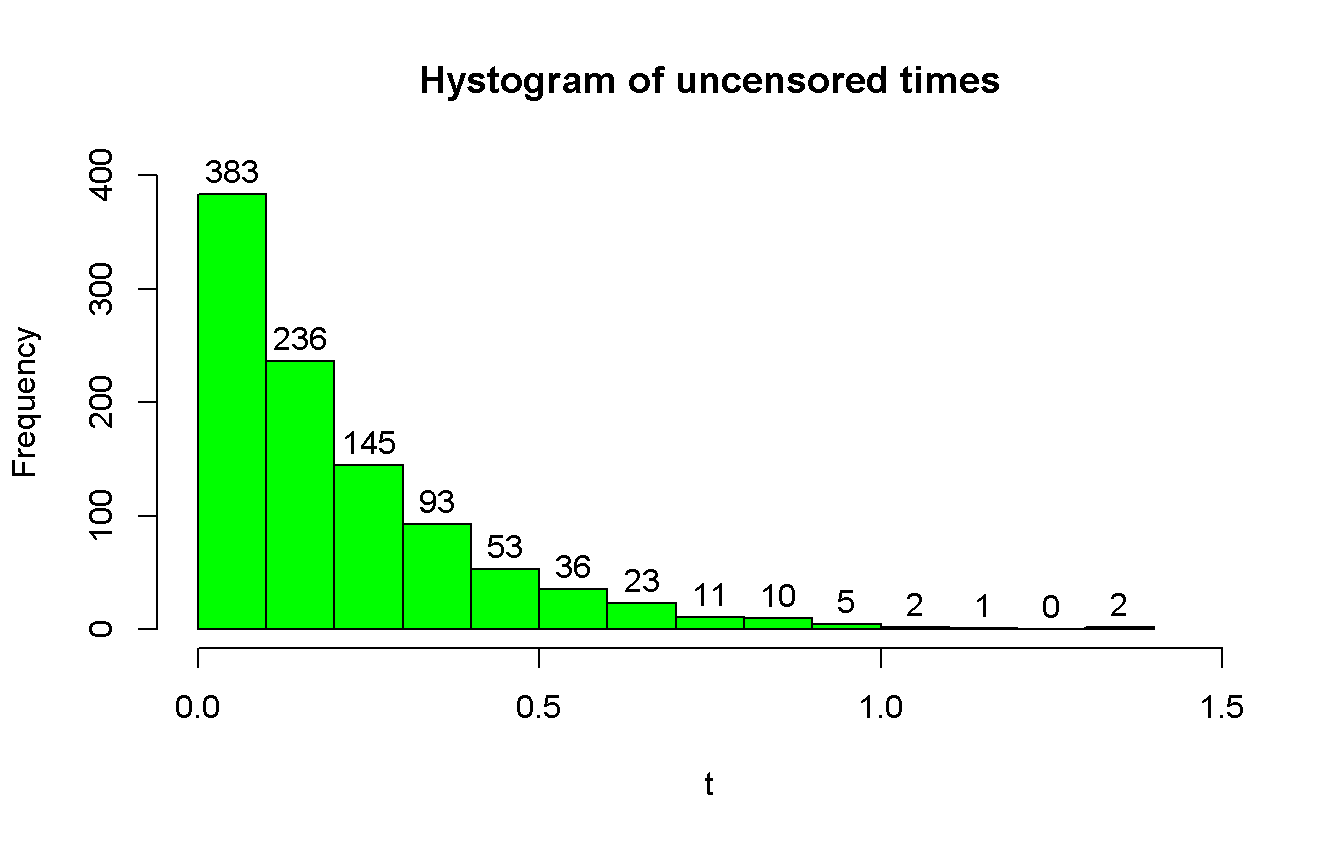
\includegraphics[width=0.5\linewidth]{SuDACDa-notes_files/figure-latex/sim_plots-1}
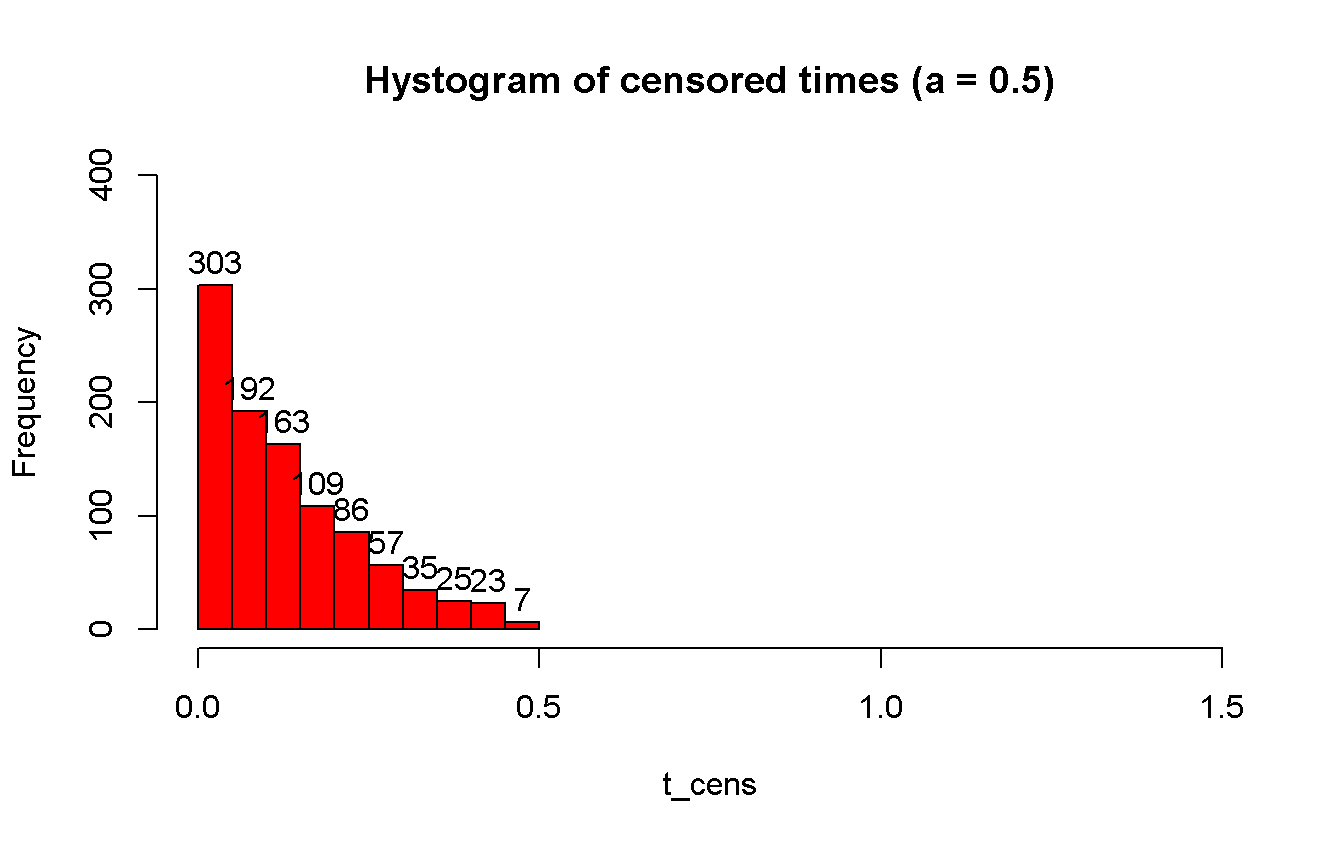
\includegraphics[width=0.5\linewidth]{SuDACDa-notes_files/figure-latex/sim_plots-2}

\begin{enumerate}
\def\labelenumi{\arabic{enumi}.}
\setcounter{enumi}{2}
\tightlist
\item
  Parametric estimation of survival function
\end{enumerate}

\begin{itemize}
\tightlist
\item
  Uncensored
\end{itemize}

\begin{Shaded}
\begin{Highlighting}[]
\CommentTok{# `?survreg` := "Regression for a Parametric Survival Model"}
\CommentTok{# }
\CommentTok{# R formula: y ~ x <--> math formula: y = f(x)}
\CommentTok{# }
\CommentTok{# Here we want to model the response (labelled time) as they are, without any}
\CommentTok{# furter investigation on the effect on them from some other variable}
\KeywordTok{survreg}\NormalTok{(}\KeywordTok{Surv}\NormalTok{(t, status_no_cens) ~}\StringTok{ }\DecValTok{1}\NormalTok{,}
  \DataTypeTok{dist =} \StringTok{'exponential'}
\NormalTok{) %>%}
\StringTok{  }\NormalTok{summary     }\CommentTok{# here `summary()` add some more statistics to the standard output}
\end{Highlighting}
\end{Shaded}

\begin{verbatim}
## 
## Call:
## survreg(formula = Surv(t, status_no_cens) ~ 1, dist = "exponential")
##             Value Std. Error     z p
## (Intercept) -1.58     0.0316 -50.1 0
## 
## Scale fixed at 1 
## 
## Exponential distribution
## Loglik(model)= 584.3   Loglik(intercept only)= 584.3
## Number of Newton-Raphson Iterations: 4 
## n= 1000
\end{verbatim}

\begin{itemize}
\tightlist
\item
  Censored
\end{itemize}

\begin{Shaded}
\begin{Highlighting}[]
\KeywordTok{survreg}\NormalTok{(}\KeywordTok{Surv}\NormalTok{(t_cens, status_cens) ~}\StringTok{ }\DecValTok{1}\NormalTok{,}
  \DataTypeTok{dist =} \StringTok{'exponential'}
\NormalTok{) %>%}
\StringTok{  }\NormalTok{summary}
\end{Highlighting}
\end{Shaded}

\begin{verbatim}
## 
## Call:
## survreg(formula = Surv(t_cens, status_cens) ~ 1, dist = "exponential")
##             Value Std. Error     z p
## (Intercept) -1.57     0.0401 -39.2 0
## 
## Scale fixed at 1 
## 
## Exponential distribution
## Loglik(model)= 355.9   Loglik(intercept only)= 355.9
## Number of Newton-Raphson Iterations: 4 
## n= 1000
\end{verbatim}

\begin{enumerate}
\def\labelenumi{\arabic{enumi}.}
\setcounter{enumi}{3}
\tightlist
\item
  Non parametric estimation of survival and the distribution functions
\end{enumerate}

\begin{itemize}
\tightlist
\item
  Uncensored
\end{itemize}

\begin{Shaded}
\begin{Highlighting}[]
\CommentTok{# `?survfit` := "Create survival curves"}
\KeywordTok{survfit}\NormalTok{(}\KeywordTok{Surv}\NormalTok{(t, status_no_cens) ~}\StringTok{ }\DecValTok{1}\NormalTok{)}
\end{Highlighting}
\end{Shaded}

\begin{verbatim}
## Call: survfit(formula = Surv(t, status_no_cens) ~ 1)
## 
##        n   events   median  0.95LCL  0.95UCL 
## 1000.000 1000.000    0.140    0.128    0.158
\end{verbatim}

\begin{Shaded}
\begin{Highlighting}[]
\CommentTok{# Here we would like to compare to approach to survival plots:}
\CommentTok{# 1. Using the packege _survival_, so the standard one}
\CommentTok{# 2. Uisng the package _rms_, a comprehensive package for regression analyses}

\CommentTok{# Using survival `plot` provided by the _survival_ package}
\CommentTok{# (`?survival:::plot.survfit`), we can continue to}
\CommentTok{# use the `survfit()` function for nonparametric survival estimation from the}
\CommentTok{# same _survival_ package}
\KeywordTok{survfit}\NormalTok{(}\KeywordTok{Surv}\NormalTok{(t, status_no_cens) ~}\StringTok{ }\DecValTok{1}\NormalTok{) %>%}\StringTok{ }
\StringTok{  }\KeywordTok{plot}\NormalTok{(}
    \DataTypeTok{xlim     =} \KeywordTok{c}\NormalTok{(}\DecValTok{0}\NormalTok{, }\FloatTok{1.55}\NormalTok{),}
    \DataTypeTok{conf.int  =} \OtherTok{TRUE}\NormalTok{,}
    \DataTypeTok{mark.time =} \OtherTok{TRUE}\NormalTok{,}
    \DataTypeTok{col       =} \StringTok{'green'}\NormalTok{,}
    \DataTypeTok{main      =} \StringTok{'Uncensored --- survival'}
\NormalTok{)}


\CommentTok{# Using the survplot from the _rms_ package (`survplot`), we have to switch to}
\CommentTok{# the `npsurv()` function for nonparametric survival estimation from the _rms_}
\CommentTok{# package}
\KeywordTok{npsurv}\NormalTok{(}\KeywordTok{Surv}\NormalTok{(t, status_no_cens) ~}\StringTok{ }\DecValTok{1}\NormalTok{) %>%}\StringTok{ }
\StringTok{  }\KeywordTok{survplot}\NormalTok{(}
    \DataTypeTok{xlim     =} \KeywordTok{c}\NormalTok{(}\DecValTok{0}\NormalTok{, }\FloatTok{1.5}\NormalTok{),}
    \DataTypeTok{conf.int =} \OtherTok{TRUE}\NormalTok{,}
    \DataTypeTok{n.risk   =} \OtherTok{TRUE}\NormalTok{,}
    \DataTypeTok{col      =} \StringTok{'green'}
\NormalTok{)}
\KeywordTok{title}\NormalTok{(}\DataTypeTok{main =} \StringTok{'Uncensored --- rms'}\NormalTok{) }\CommentTok{# unfortunally survplot do not have an}
                                   \CommentTok{# integrated option for the title...}
\end{Highlighting}
\end{Shaded}

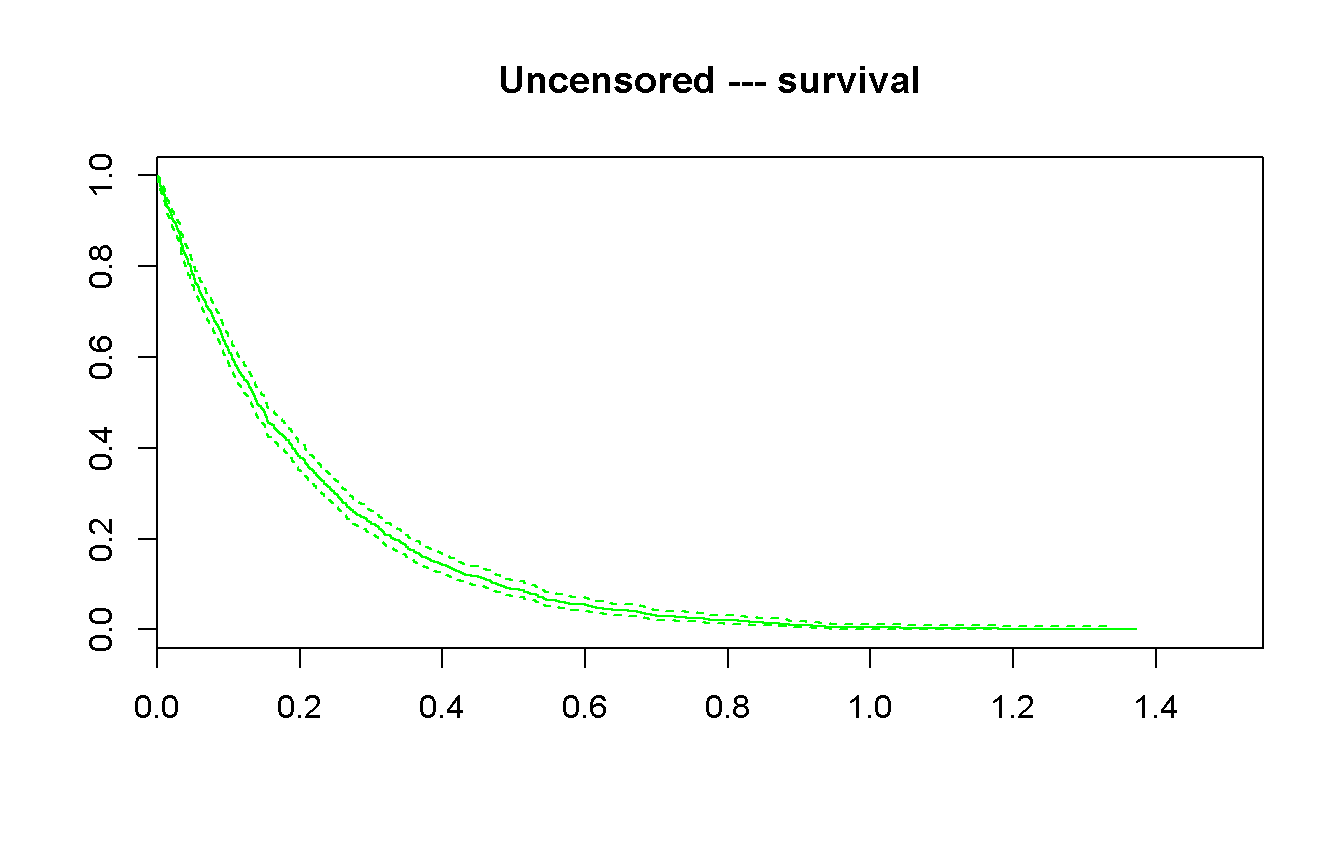
\includegraphics{SuDACDa-notes_files/figure-latex/survfit_nocens-1.pdf}
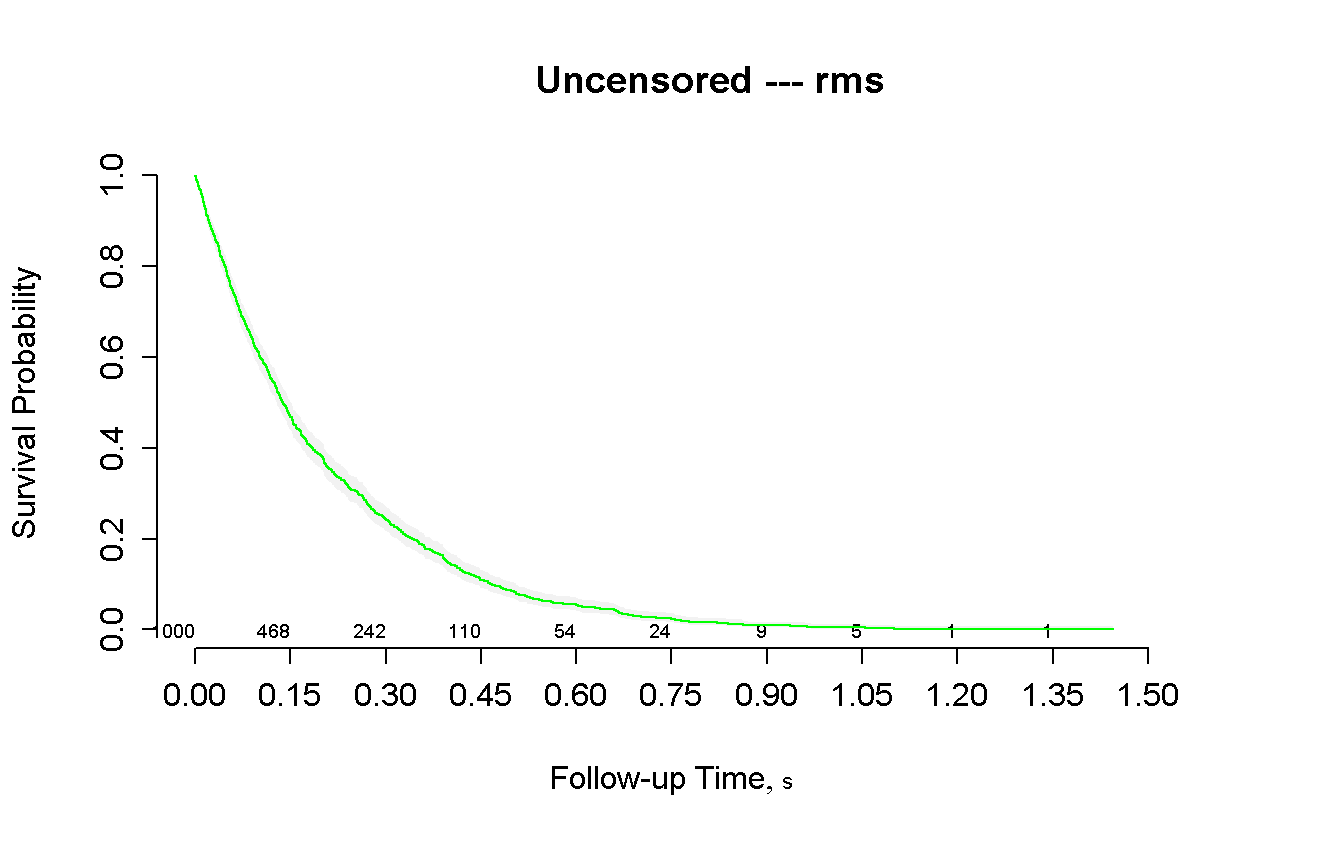
\includegraphics{SuDACDa-notes_files/figure-latex/survfit_nocens-2.pdf}

\begin{itemize}
\tightlist
\item
  censored
\end{itemize}

\begin{Shaded}
\begin{Highlighting}[]
\KeywordTok{survfit}\NormalTok{(}\KeywordTok{Surv}\NormalTok{(t_cens, status_cens) ~}\StringTok{ }\DecValTok{1}\NormalTok{)}
\end{Highlighting}
\end{Shaded}

\begin{verbatim}
## Call: survfit(formula = Surv(t_cens, status_cens) ~ 1)
## 
##        n   events   median  0.95LCL  0.95UCL 
## 1000.000  623.000    0.141    0.130    0.158
\end{verbatim}

\begin{Shaded}
\begin{Highlighting}[]
\KeywordTok{survfit}\NormalTok{(}\KeywordTok{Surv}\NormalTok{(t_cens, status_cens) ~}\StringTok{ }\DecValTok{1}\NormalTok{) %>%}
\StringTok{  }\KeywordTok{plot}\NormalTok{(}
    \DataTypeTok{xlim     =} \KeywordTok{c}\NormalTok{(}\DecValTok{0}\NormalTok{, }\FloatTok{0.55}\NormalTok{),}
    \DataTypeTok{conf.int  =} \OtherTok{TRUE}\NormalTok{,}
    \DataTypeTok{mark.time =} \OtherTok{TRUE}\NormalTok{,}
    \DataTypeTok{col      =} \StringTok{'red'}\NormalTok{,}
    \DataTypeTok{main      =} \StringTok{'Censored (a = 0.5)'}
\NormalTok{)}

\KeywordTok{npsurv}\NormalTok{(}\KeywordTok{Surv}\NormalTok{(t_cens, status_cens) ~}\StringTok{ }\DecValTok{1}\NormalTok{) %>%}\StringTok{ }
\StringTok{  }\KeywordTok{survplot}\NormalTok{(}
    \DataTypeTok{xlim     =} \KeywordTok{c}\NormalTok{(}\DecValTok{0}\NormalTok{, }\FloatTok{0.5}\NormalTok{),}
    \DataTypeTok{conf.int =} \OtherTok{TRUE}\NormalTok{,}
    \DataTypeTok{n.risk   =} \OtherTok{TRUE}\NormalTok{,}
    \DataTypeTok{col      =} \StringTok{'red'}
\NormalTok{)}
\KeywordTok{title}\NormalTok{(}\DataTypeTok{main =} \StringTok{'Censored (a = 0.5) --- rms'}\NormalTok{)}
\end{Highlighting}
\end{Shaded}

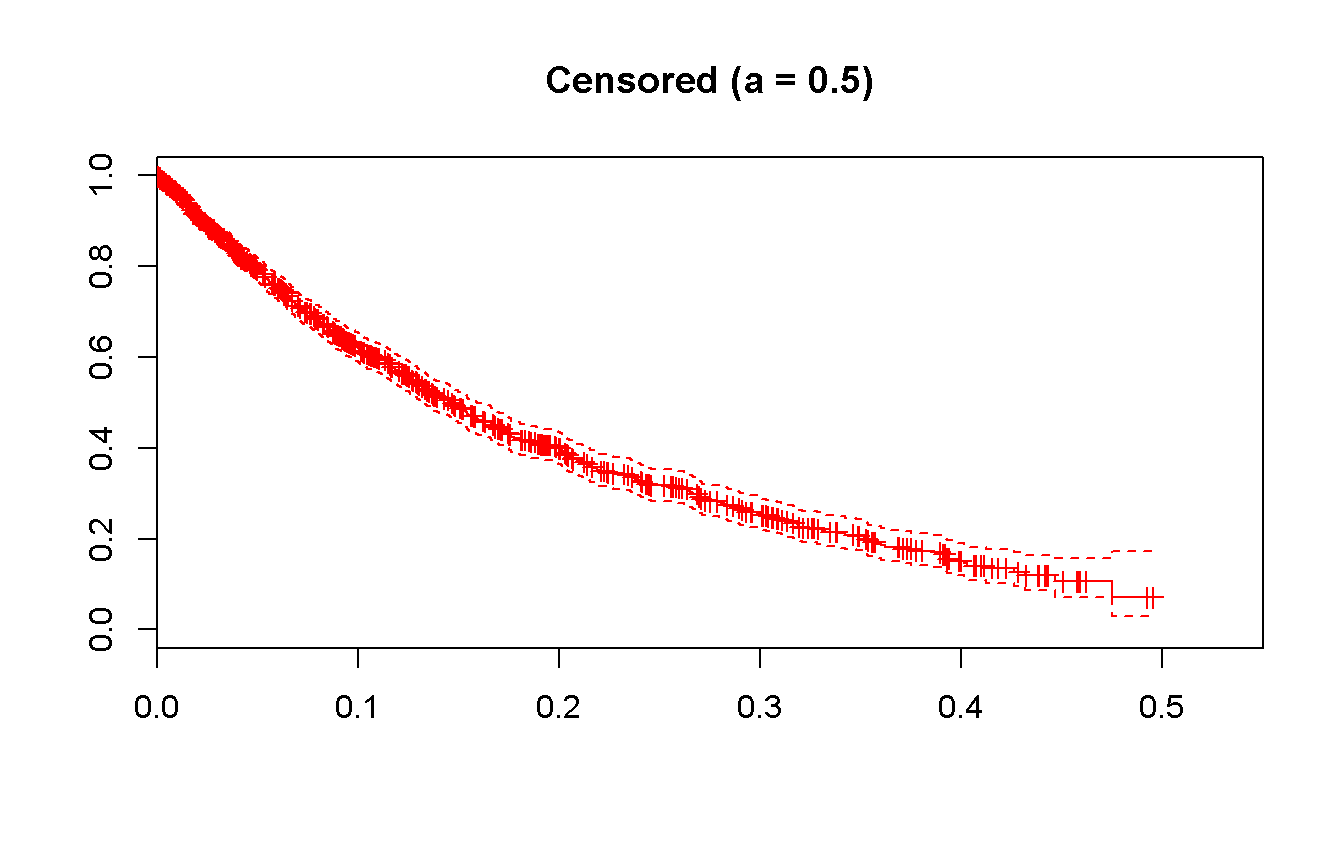
\includegraphics{SuDACDa-notes_files/figure-latex/survfit_cens-1.pdf}
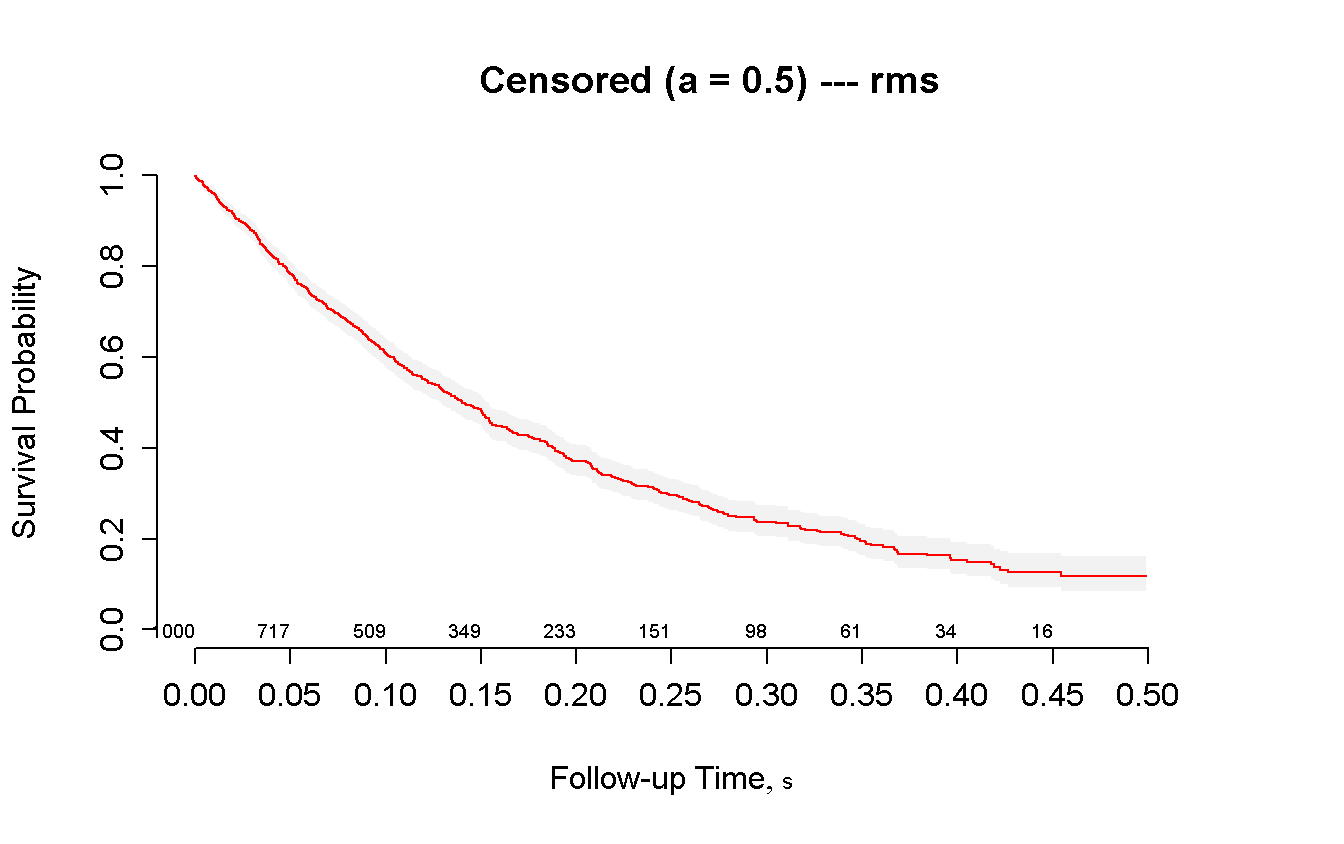
\includegraphics{SuDACDa-notes_files/figure-latex/survfit_cens-2.pdf}

\section{\texorpdfstring{\texttt{mgus} data from \textbf{survival}
package}{mgus data from survival package}}\label{mgus}

\begin{enumerate}
\def\labelenumi{\arabic{enumi}.}
\tightlist
\item
  Load and explore data
\end{enumerate}

\begin{Shaded}
\begin{Highlighting}[]
\KeywordTok{data}\NormalTok{(mgus)                                                                }\CommentTok{# load}
\KeywordTok{head}\NormalTok{(mgus)                                                       }\CommentTok{# first 10 rows}
\end{Highlighting}
\end{Shaded}

\begin{verbatim}
##   id age    sex dxyr pcdx pctime futime death alb creat  hgb mspike
## 1  1  78 female   68 <NA>     NA    748     1 2.8   1.2 11.5    2.0
## 2  2  73 female   66   LP   1310   6751     1  NA    NA   NA    1.3
## 3  3  87   male   68 <NA>     NA    277     1 2.2   1.1 11.2    1.3
## 4  4  86   male   69 <NA>     NA   1815     1 2.8   1.3 15.3    1.8
## 5  5  74 female   68 <NA>     NA   2587     1 3.0   0.8  9.8    1.4
## 6  6  81   male   68 <NA>     NA    563     1 2.9   0.9 11.5    1.8
\end{verbatim}

\begin{Shaded}
\begin{Highlighting}[]
\KeywordTok{dim}\NormalTok{(mgus)                                              }\CommentTok{# number of rows and cols}
\end{Highlighting}
\end{Shaded}

\begin{verbatim}
## [1] 241  12
\end{verbatim}

\begin{Shaded}
\begin{Highlighting}[]
\KeywordTok{names}\NormalTok{(mgus)                                                }\CommentTok{# name of the columns}
\end{Highlighting}
\end{Shaded}

\begin{verbatim}
##  [1] "id"     "age"    "sex"    "dxyr"   "pcdx"   "pctime" "futime"
##  [8] "death"  "alb"    "creat"  "hgb"    "mspike"
\end{verbatim}

\begin{Shaded}
\begin{Highlighting}[]
\KeywordTok{str}\NormalTok{(mgus)                                   }\CommentTok{# R internal structure of the object}
\end{Highlighting}
\end{Shaded}

\begin{verbatim}
## 'data.frame':    241 obs. of  12 variables:
##  $ id    : num  1 2 3 4 5 6 7 8 9 10 ...
##  $ age   : atomic  78 73 87 86 74 81 72 79 85 58 ...
##   ..- attr(*, "label")= chr "AGE AT date_on"
##  $ sex   : Factor w/ 2 levels "female","male": 1 1 2 2 1 2 1 1 1 2 ...
##   ..- attr(*, "label")= chr "Sex"
##  $ dxyr  : num  68 66 68 69 68 68 68 69 70 65 ...
##  $ pcdx  : Factor w/ 4 levels "AM","LP","MA",..: NA 2 NA NA NA NA NA NA NA NA ...
##  $ pctime: atomic  NA 1310 NA NA NA NA NA NA NA NA ...
##   ..- attr(*, "label")= chr "Progression to Group 4 (days)"
##  $ futime: atomic  748 6751 277 1815 2587 ...
##   ..- attr(*, "label")= chr "Follow-Up Time"
##  $ death : num  1 1 1 1 1 1 1 1 1 1 ...
##  $ alb   : atomic  2.8 NA 2.2 2.8 3 2.9 3 3.1 3.2 3.5 ...
##   ..- attr(*, "label")= chr "Serum Albumin"
##  $ creat : atomic  1.2 NA 1.1 1.3 0.8 0.9 0.8 0.8 1 1 ...
##   ..- attr(*, "label")= chr "Serum Creatinine"
##  $ hgb   : atomic  11.5 NA 11.2 15.3 9.8 11.5 13.5 15.5 12.4 14.8 ...
##   ..- attr(*, "label")= chr "Hemoglobin"
##  $ mspike: atomic  2 1.3 1.3 1.8 1.4 1.8 1.3 1.4 1.5 2.2 ...
##   ..- attr(*, "label")= chr "Serum M-Spike"
##  - attr(*, "formats")=List of 1
##   ..$ death:List of 2
##   .. ..$ values: num  0 1
##   .. ..$ labels: chr  "Alive" "Dead"
\end{verbatim}

\begin{Shaded}
\begin{Highlighting}[]
\KeywordTok{summary}\NormalTok{(mgus)                                              }\CommentTok{# summary from base R}
\end{Highlighting}
\end{Shaded}

\begin{verbatim}
##        id           age            sex           dxyr        pcdx    
##  Min.   :  1   Min.   :34.00   female:104   Min.   :56.0   AM  :  8  
##  1st Qu.: 61   1st Qu.:55.00   male  :137   1st Qu.:66.0   LP  :  5  
##  Median :121   Median :63.00                Median :68.0   MA  :  7  
##  Mean   :121   Mean   :62.87                Mean   :67.4   MM  : 44  
##  3rd Qu.:181   3rd Qu.:72.00                3rd Qu.:70.0   NA's:177  
##  Max.   :241   Max.   :90.00                Max.   :73.0             
##                                                                      
##      pctime          futime          death             alb       
##  Min.   :  365   Min.   :    6   Min.   :0.0000   Min.   :1.800  
##  1st Qu.: 2469   1st Qu.: 2422   1st Qu.:1.0000   1st Qu.:2.900  
##  Median : 3778   Median : 5022   Median :1.0000   Median :3.200  
##  Mean   : 4342   Mean   : 5425   Mean   :0.9336   Mean   :3.204  
##  3rd Qu.: 5750   3rd Qu.: 8264   3rd Qu.:1.0000   3rd Qu.:3.500  
##  Max.   :11685   Max.   :14325   Max.   :1.0000   Max.   :5.100  
##  NA's   :177                                      NA's   :31     
##      creat            hgb            mspike     
##  Min.   :0.600   Min.   : 7.40   Min.   :0.300  
##  1st Qu.:0.900   1st Qu.:12.20   1st Qu.:1.500  
##  Median :1.000   Median :13.20   Median :1.700  
##  Mean   :1.095   Mean   :13.15   Mean   :1.764  
##  3rd Qu.:1.100   3rd Qu.:14.50   3rd Qu.:2.000  
##  Max.   :6.400   Max.   :16.60   Max.   :3.200  
##  NA's   :43      NA's   :1
\end{verbatim}

\begin{Shaded}
\begin{Highlighting}[]
\KeywordTok{describe}\NormalTok{(mgus)   }\CommentTok{# more comprehensive description from _Hisc_ package, loaded by}
\end{Highlighting}
\end{Shaded}

\begin{verbatim}
## mgus 
## 
##  12  Variables      241  Observations
## ---------------------------------------------------------------------------
## id 
##        n  missing distinct     Info     Mean      Gmd      .05      .10 
##      241        0      241        1      121    80.67       13       25 
##      .25      .50      .75      .90      .95 
##       61      121      181      217      229 
## 
## lowest :   1   2   3   4   5, highest: 237 238 239 240 241
## ---------------------------------------------------------------------------
## age : AGE AT date_on 
##        n  missing distinct     Info     Mean      Gmd      .05      .10 
##      241        0       53    0.999    62.87    13.42       44       48 
##      .25      .50      .75      .90      .95 
##       55       63       72       78       81 
## 
## lowest : 34 35 36 37 38, highest: 84 85 86 87 90
## ---------------------------------------------------------------------------
## sex : Sex 
##        n  missing distinct 
##      241        0        2 
##                         
## Value      female   male
## Frequency     104    137
## Proportion  0.432  0.568
## ---------------------------------------------------------------------------
## dxyr 
##        n  missing distinct     Info     Mean      Gmd      .05      .10 
##      241        0       17     0.97     67.4    3.073       61       63 
##      .25      .50      .75      .90      .95 
##       66       68       70       70       70 
##                                                                       
## Value         56    58    59    60    61    62    63    64    65    66
## Frequency      1     1     5     5     2     7     7    10    10    18
## Proportion 0.004 0.004 0.021 0.021 0.008 0.029 0.029 0.041 0.041 0.075
##                                                     
## Value         67    68    69    70    71    72    73
## Frequency     24    40    45    62     2     1     1
## Proportion 0.100 0.166 0.187 0.257 0.008 0.004 0.004
## ---------------------------------------------------------------------------
## pcdx 
##        n  missing distinct 
##       64      177        4 
##                                   
## Value         AM    LP    MA    MM
## Frequency      8     5     7    44
## Proportion 0.125 0.078 0.109 0.688
## ---------------------------------------------------------------------------
## pctime : Progression to Group 4 (days) 
##        n  missing distinct     Info     Mean      Gmd      .05      .10 
##       64      177       63        1     4342     3030     1223     1409 
##      .25      .50      .75      .90      .95 
##     2469     3778     5750     8946    10051 
## 
## lowest :   365   700   954  1218  1249, highest:  9723 10109 10359 11354 11685
## ---------------------------------------------------------------------------
## futime : Follow-Up Time 
##        n  missing distinct     Info     Mean      Gmd      .05      .10 
##      241        0      237        1     5425     4222      283      779 
##      .25      .50      .75      .90      .95 
##     2422     5022     8264    11425    12140 
## 
## lowest :     6     7    31    32    39, highest: 12931 13019 13152 14111 14325
## ---------------------------------------------------------------------------
## death 
##        n  missing distinct     Info      Sum     Mean      Gmd 
##      241        0        2    0.186      225   0.9336   0.1245 
## 
## ---------------------------------------------------------------------------
## alb : Serum Albumin 
##        n  missing distinct     Info     Mean      Gmd      .05      .10 
##      210       31       26    0.995    3.204   0.5293      2.3      2.6 
##      .25      .50      .75      .90      .95 
##      2.9      3.2      3.5      3.8      3.9 
## 
## lowest : 1.8 1.9 2.1 2.2 2.3, highest: 4.0 4.1 4.3 4.5 5.1
## ---------------------------------------------------------------------------
## creat : Serum Creatinine 
##        n  missing distinct     Info     Mean      Gmd      .05      .10 
##      198       43       19    0.978    1.095     0.39    0.700    0.800 
##      .25      .50      .75      .90      .95 
##    0.900    1.000    1.100    1.300    1.615 
##                                                                       
## Value        0.6   0.7   0.8   0.9   1.0   1.1   1.2   1.3   1.4   1.5
## Frequency      4    13    26    42    35    29    18    12     4     4
## Proportion 0.020 0.066 0.131 0.212 0.177 0.146 0.091 0.061 0.020 0.020
##                                                                 
## Value        1.6   1.7   2.0   2.5   2.6   3.5   3.6   3.7   6.4
## Frequency      1     3     1     1     1     1     1     1     1
## Proportion 0.005 0.015 0.005 0.005 0.005 0.005 0.005 0.005 0.005
## ---------------------------------------------------------------------------
## hgb : Hemoglobin 
##        n  missing distinct     Info     Mean      Gmd      .05      .10 
##      240        1       66    0.999    13.15    1.865    10.20    11.09 
##      .25      .50      .75      .90      .95 
##    12.20    13.20    14.50    15.11    15.51 
## 
## lowest :  7.4  7.7  8.4  9.5  9.6, highest: 15.9 16.1 16.2 16.5 16.6
## ---------------------------------------------------------------------------
## mspike : Serum M-Spike 
##        n  missing distinct     Info     Mean      Gmd      .05      .10 
##      241        0       23    0.993    1.764   0.4687      1.1      1.3 
##      .25      .50      .75      .90      .95 
##      1.5      1.7      2.0      2.3      2.5 
## 
## lowest : 0.3 0.8 0.9 1.0 1.1, highest: 2.5 2.6 2.7 2.9 3.2
## ---------------------------------------------------------------------------
\end{verbatim}

\begin{Shaded}
\begin{Highlighting}[]
                 \CommentTok{# the _rms_ one}

\NormalTok{mgus_df <-}\StringTok{ }\KeywordTok{as_tibble}\NormalTok{(mgus)         }\CommentTok{# tidy data frame (important info printed all}
                                   \CommentTok{# together, and visualization auto-adjusted}
                                   \CommentTok{# to the consol width)}
\NormalTok{mgus_df}
\end{Highlighting}
\end{Shaded}

\begin{verbatim}
## # A tibble: 241 x 12
##       id   age    sex  dxyr   pcdx pctime futime death   alb creat   hgb
##  * <dbl> <dbl> <fctr> <dbl> <fctr>  <dbl>  <dbl> <dbl> <dbl> <dbl> <dbl>
##  1     1    78 female    68   <NA>     NA    748     1   2.8   1.2  11.5
##  2     2    73 female    66     LP   1310   6751     1    NA    NA    NA
##  3     3    87   male    68   <NA>     NA    277     1   2.2   1.1  11.2
##  4     4    86   male    69   <NA>     NA   1815     1   2.8   1.3  15.3
##  5     5    74 female    68   <NA>     NA   2587     1   3.0   0.8   9.8
##  6     6    81   male    68   <NA>     NA    563     1   2.9   0.9  11.5
##  7     7    72 female    68   <NA>     NA   1135     1   3.0   0.8  13.5
##  8     8    79 female    69   <NA>     NA   2016     1   3.1   0.8  15.5
##  9     9    85 female    70   <NA>     NA   2422     1   3.2   1.0  12.4
## 10    10    58   male    65   <NA>     NA   6155     1   3.5   1.0  14.8
## # ... with 231 more rows, and 1 more variables: mspike <dbl>
\end{verbatim}

\begin{enumerate}
\def\labelenumi{\arabic{enumi}.}
\setcounter{enumi}{1}
\tightlist
\item
  Non parametric Kaplan-Meyer estimation of the survival function
\end{enumerate}

\begin{itemize}
\tightlist
\item
  Estimate the survival function from randomization overall and
  according to sex.
\end{itemize}

\begin{Shaded}
\begin{Highlighting}[]
\KeywordTok{survfit}\NormalTok{(}\KeywordTok{Surv}\NormalTok{(futime, death) ~}\StringTok{ }\DecValTok{1}\NormalTok{,}
  \DataTypeTok{data =} \NormalTok{mgus_df}
\NormalTok{) %>%}
\StringTok{  }\KeywordTok{plot}\NormalTok{(}
    \DataTypeTok{conf.int  =} \OtherTok{TRUE}\NormalTok{,}
    \DataTypeTok{mark.time =} \OtherTok{TRUE}\NormalTok{,}
    \DataTypeTok{col       =} \StringTok{'blue'}\NormalTok{,}
    \DataTypeTok{main      =} \StringTok{'Survival function for mgus data'}
\NormalTok{)}


\KeywordTok{survfit}\NormalTok{(}\KeywordTok{Surv}\NormalTok{(futime, death) ~}\StringTok{ }\NormalTok{sex,}
  \DataTypeTok{data =} \NormalTok{mgus_df}
\NormalTok{) %>%}
\StringTok{  }\KeywordTok{plot}\NormalTok{(}
    \DataTypeTok{conf.int  =} \OtherTok{TRUE}\NormalTok{,}
    \DataTypeTok{mark.time =} \OtherTok{TRUE}\NormalTok{,}
    \DataTypeTok{main      =} \StringTok{'Survival function for mgus data according to sex'}\NormalTok{,}
    \DataTypeTok{col       =} \KeywordTok{c}\NormalTok{(}\StringTok{'red'}\NormalTok{, }\StringTok{'blue'}\NormalTok{),}
    \DataTypeTok{lty       =} \KeywordTok{c}\NormalTok{(}\DecValTok{2}\NormalTok{, }\DecValTok{3}\NormalTok{)}
\NormalTok{)}
\KeywordTok{legend}\NormalTok{(}
  \DataTypeTok{x =} \DecValTok{10000}\NormalTok{, }\DataTypeTok{y =} \DecValTok{1}\NormalTok{,}
  \DataTypeTok{legend =} \KeywordTok{c}\NormalTok{(}\StringTok{"Female"}\NormalTok{, }\StringTok{"Male"}\NormalTok{),}
  \DataTypeTok{col    =} \KeywordTok{c}\NormalTok{(}\StringTok{'red'}\NormalTok{, }\StringTok{'blue'}\NormalTok{),}
  \DataTypeTok{lty    =} \KeywordTok{c}\NormalTok{(}\DecValTok{2}\NormalTok{, }\DecValTok{3}\NormalTok{)}
\NormalTok{)}
\end{Highlighting}
\end{Shaded}

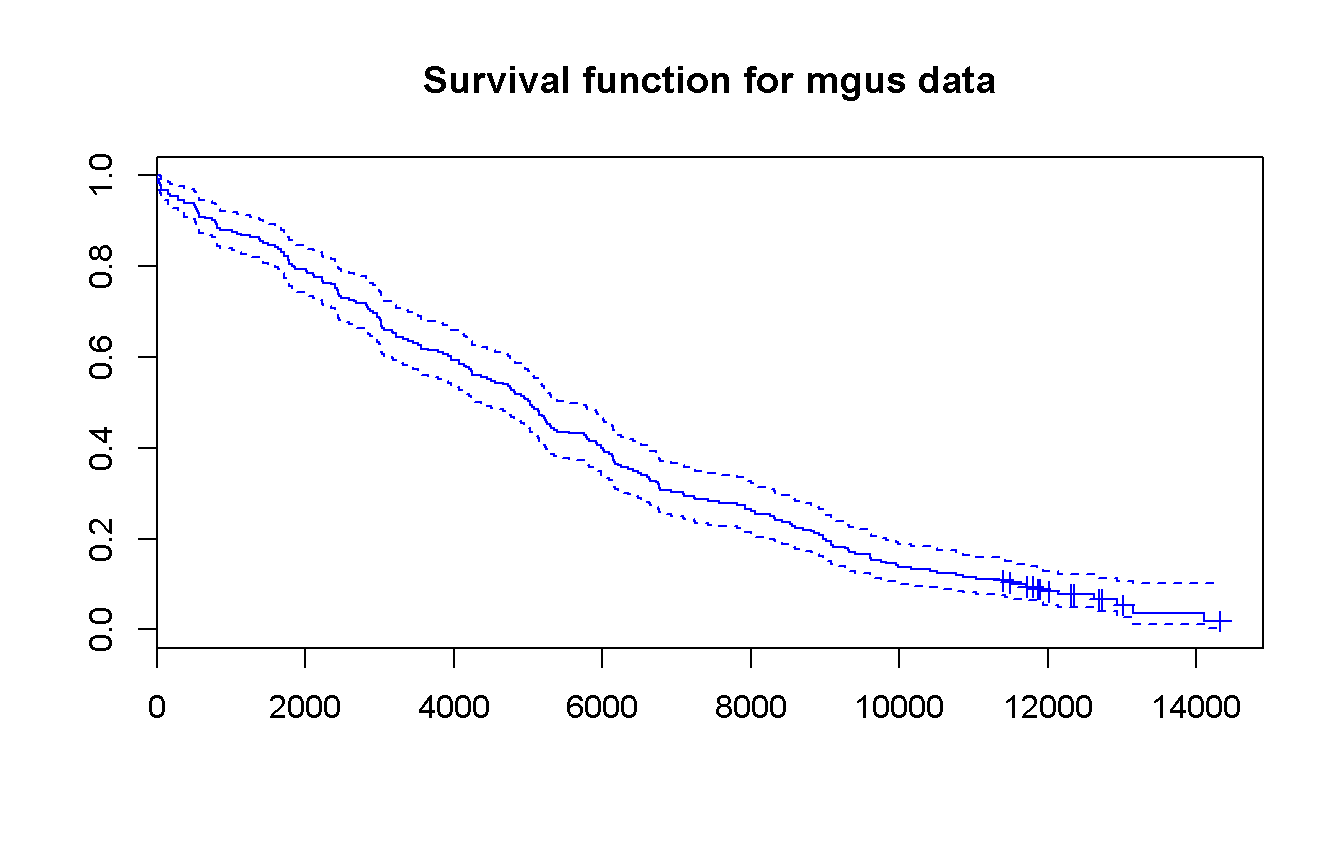
\includegraphics{SuDACDa-notes_files/figure-latex/rmgus_survfit-1.pdf}
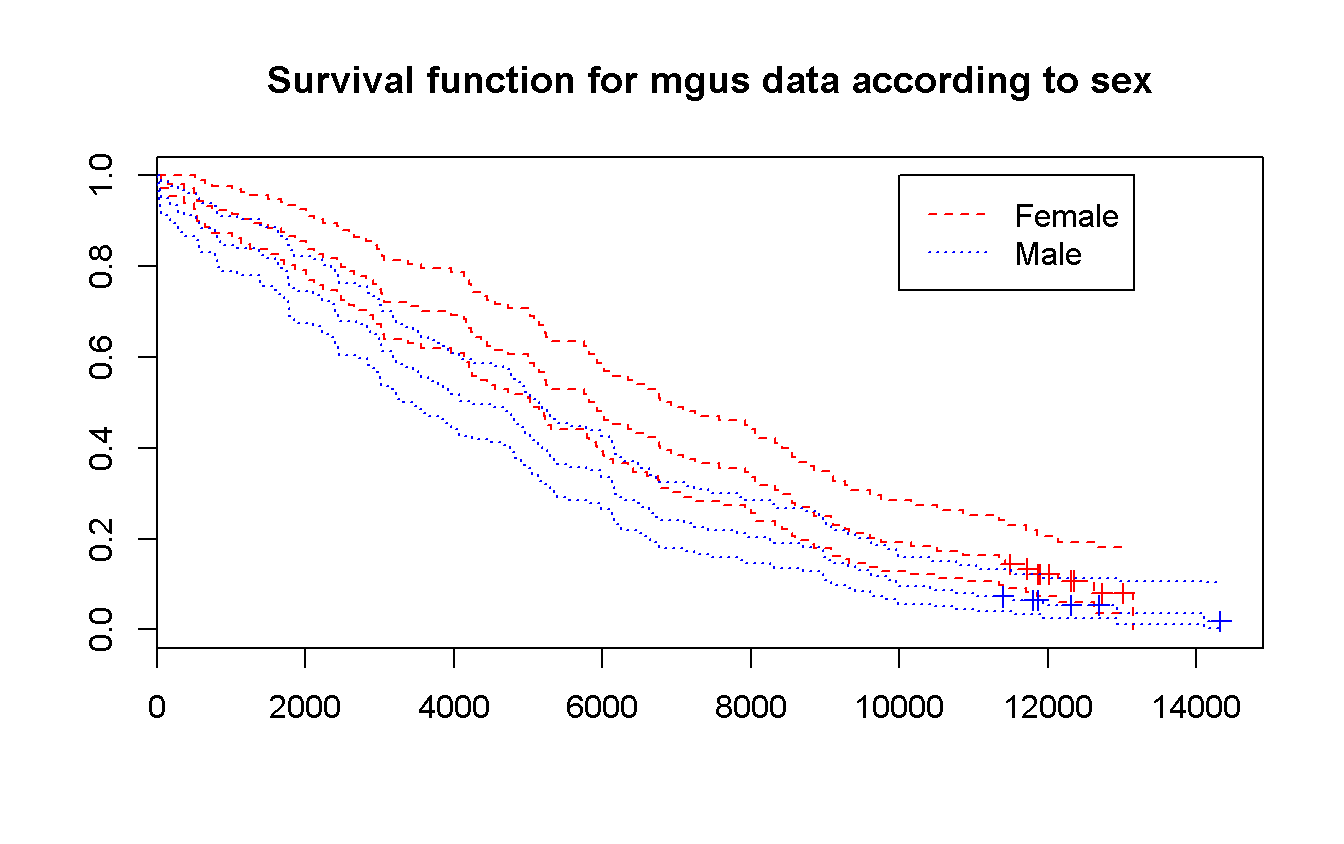
\includegraphics{SuDACDa-notes_files/figure-latex/rmgus_survfit-2.pdf}

\begin{Shaded}
\begin{Highlighting}[]
\CommentTok{# For survival object the package _survminer_ provide ggplot2 plots}
\CommentTok{# (`?ggsurvplot`) which could be very interesting and quite comprehensive.}

\KeywordTok{survfit}\NormalTok{(}\KeywordTok{Surv}\NormalTok{(futime, death) ~}\StringTok{ }\NormalTok{sex,}
  \DataTypeTok{data =} \NormalTok{mgus_df}
\NormalTok{) %>%}\StringTok{ }
\StringTok{  }\KeywordTok{ggsurvplot}\NormalTok{(}
    \DataTypeTok{conf.int            =} \OtherTok{TRUE}\NormalTok{,                      }\CommentTok{# draw confidence intervals}
    \DataTypeTok{pval                =} \OtherTok{TRUE}\NormalTok{,                                    }\CommentTok{# show pvalue}
    \DataTypeTok{pval.method         =} \OtherTok{TRUE}\NormalTok{,                            }\CommentTok{# print the test name}
    \DataTypeTok{title               =} \StringTok{'Survival curves for overall death according to sex.'}\NormalTok{,}
    \DataTypeTok{xlab                =} \StringTok{'Days'}\NormalTok{,}
    \DataTypeTok{legend              =} \StringTok{'right'}\NormalTok{,                             }\CommentTok{# legend position}
    \DataTypeTok{legend.title        =} \StringTok{'Sex'}\NormalTok{,}
    \DataTypeTok{legend.labs         =} \KeywordTok{c}\NormalTok{(}\StringTok{'Female'}\NormalTok{, }\StringTok{'Male'}\NormalTok{),}
    \DataTypeTok{risk.table          =} \OtherTok{TRUE}\NormalTok{,     }\CommentTok{# admits interesting options other than TRUE}
    \DataTypeTok{cumcensor           =} \OtherTok{TRUE}\NormalTok{,}
    \DataTypeTok{cumevents           =} \OtherTok{TRUE}\NormalTok{,}
    \DataTypeTok{pval.size           =} \FloatTok{3.5}\NormalTok{,   }\CommentTok{# from here these are options passed to `ggpar`}
    \DataTypeTok{risk.table.fontsize =} \DecValTok{3}\NormalTok{,     }\CommentTok{# for a better visualization}
    \DataTypeTok{fontsize            =} \DecValTok{3}\NormalTok{,     }\CommentTok{# (auto-explicatives)}
    \DataTypeTok{xscale              =} \FloatTok{30.44}
  \NormalTok{)}
\end{Highlighting}
\end{Shaded}

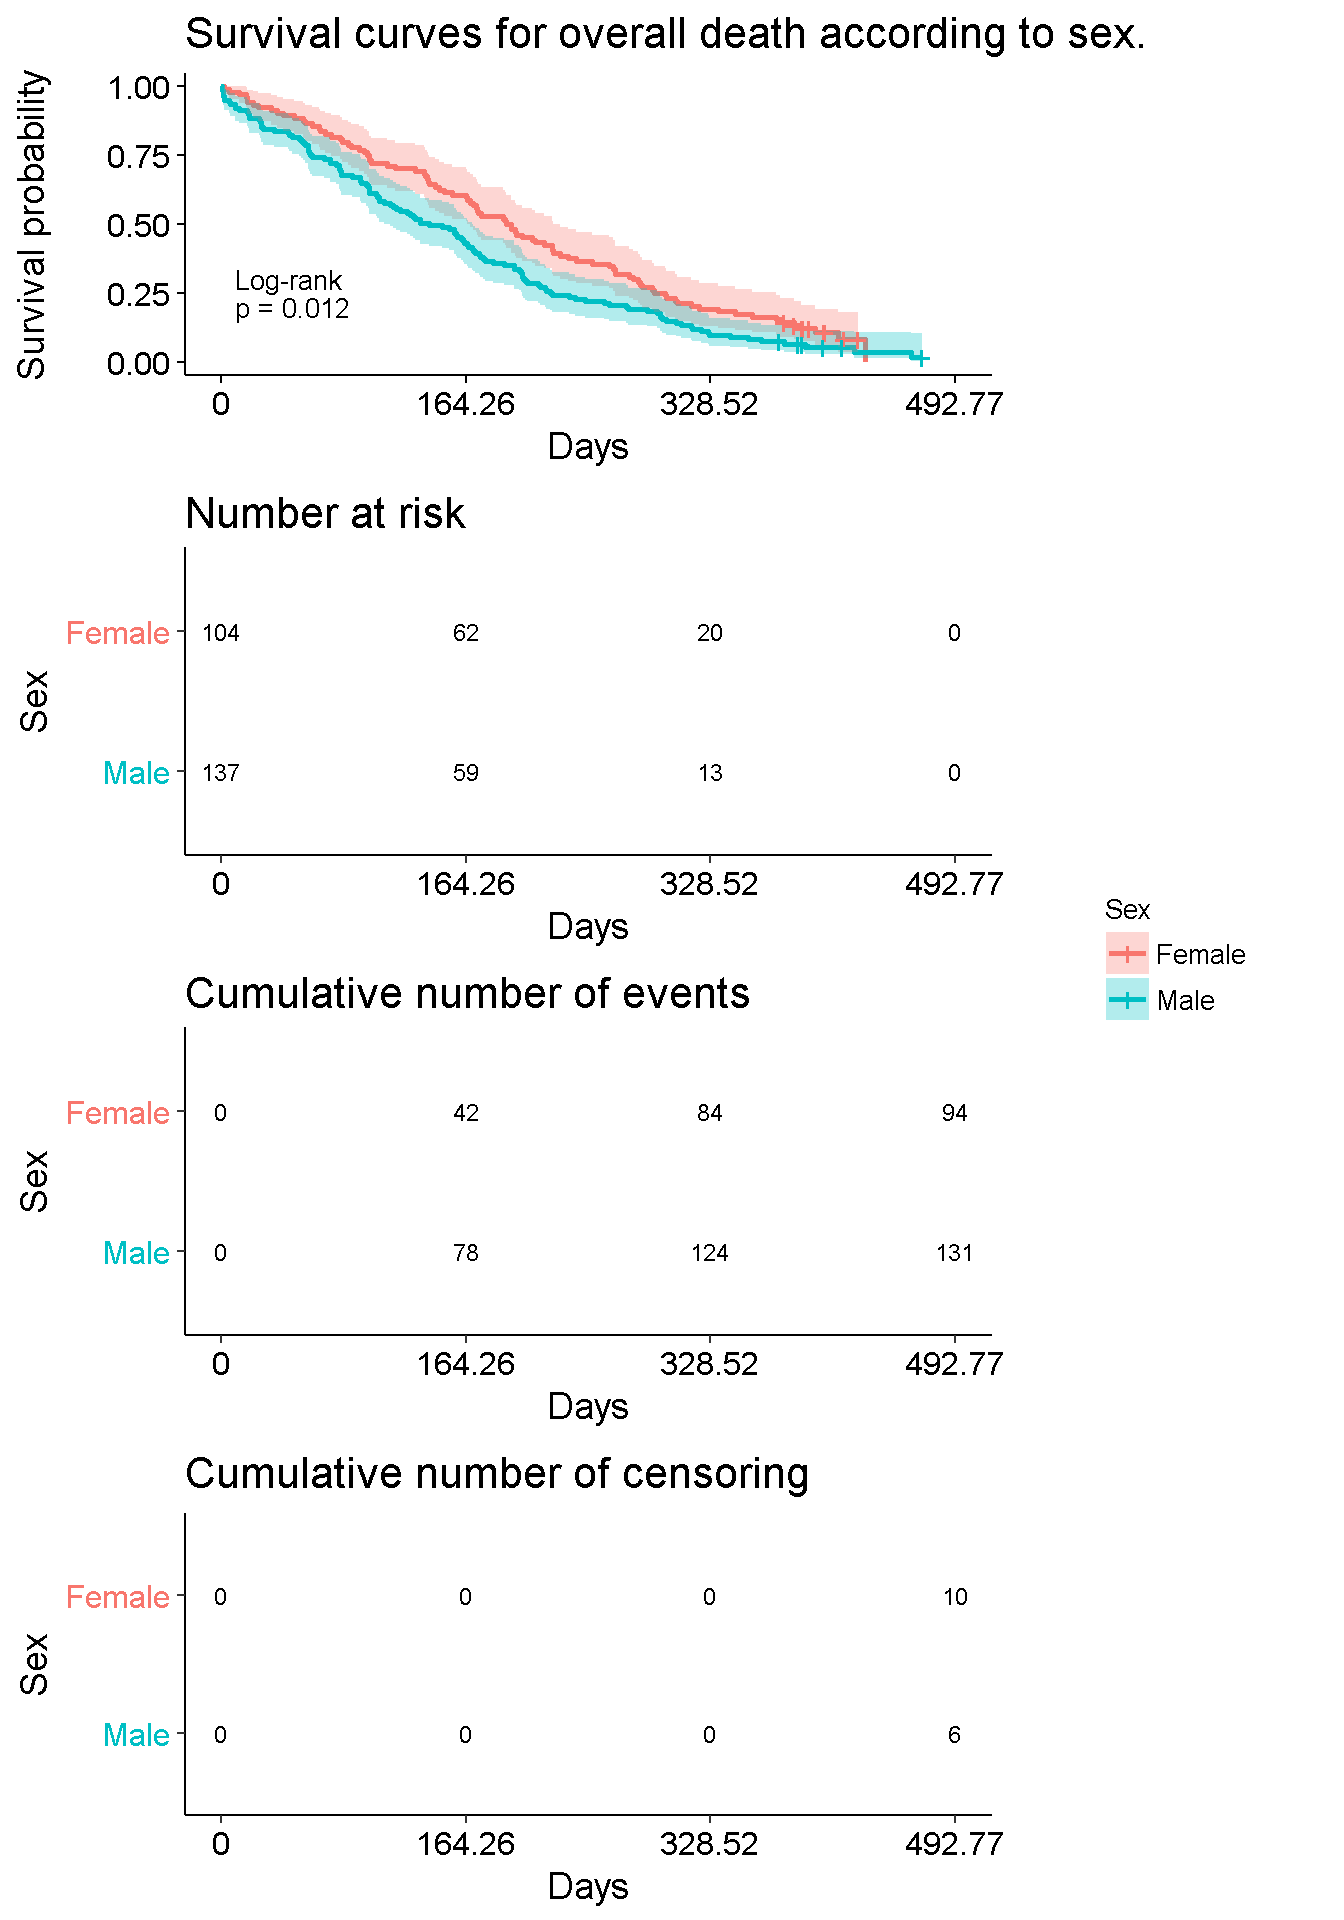
\includegraphics{SuDACDa-notes_files/figure-latex/rmgus_survminer-1.pdf}

\begin{quote}
Note: No female reaches the end of the f-up!
\end{quote}

\begin{itemize}
\tightlist
\item
  Test the effect of sex
\end{itemize}

\begin{Shaded}
\begin{Highlighting}[]
\CommentTok{# Using __survival__ (no plot method is provided for this solution)}
\KeywordTok{survdiff}\NormalTok{(}\KeywordTok{Surv}\NormalTok{(futime, death) ~}\StringTok{ }\NormalTok{sex,}
  \DataTypeTok{data =} \NormalTok{mgus_df}
\NormalTok{)}
\end{Highlighting}
\end{Shaded}

\begin{verbatim}
## Call:
## survdiff(formula = Surv(futime, death) ~ sex, data = mgus_df)
## 
##              N Observed Expected (O-E)^2/E (O-E)^2/V
## sex=female 104       94      113      3.08      6.25
## sex=male   137      131      112      3.08      6.25
## 
##  Chisq= 6.2  on 1 degrees of freedom, p= 0.0124
\end{verbatim}

\begin{Shaded}
\begin{Highlighting}[]
\CommentTok{# using __rms__}
\NormalTok{dd <-}\StringTok{ }\KeywordTok{datadist}\NormalTok{(mgus_df)  }\CommentTok{# To evaluate cph, _rms_ needs this object which simply}
                         \CommentTok{# store statistics about the data.}
                         \CommentTok{# }
                         \CommentTok{# Note: the name of the object (i.e. "dd") has to be }
                         \CommentTok{#       exactly the same as the one specified into the}
                         \CommentTok{#       option set just after the `library(rms)` call.}
                         \CommentTok{#       (See: Chapter settings) }
\NormalTok{cox_model <-}\StringTok{ }\KeywordTok{cph}\NormalTok{(}\KeywordTok{Surv}\NormalTok{(futime, death) ~}\StringTok{ }\NormalTok{sex,}
  \DataTypeTok{data  =} \NormalTok{mgus_df}
\NormalTok{)}

\KeywordTok{summary}\NormalTok{(cox_model)                           }\CommentTok{# return effect size and HR with CI}
\end{Highlighting}
\end{Shaded}

\begin{verbatim}
##              Effects              Response : Surv(futime, death) 
## 
##  Factor            Low High Diff. Effect   S.E.    Lower 0.95 Upper 0.95
##  sex - female:male 2   1    NA    -0.33853 0.13603 -0.60514   -0.071916 
##   Hazard Ratio     2   1    NA     0.71282      NA  0.54600    0.930610
\end{verbatim}

\begin{Shaded}
\begin{Highlighting}[]
\KeywordTok{Predict}\NormalTok{(cox_model) %>%}\StringTok{          }\CommentTok{# Compute predicted values and confidence limits}
\StringTok{                                }\CommentTok{#}
\StringTok{                                }\CommentTok{# Note: pay attention to Title-case "P"redict}
\StringTok{  }\KeywordTok{plot}\NormalTok{(}
    \DataTypeTok{groups =} \StringTok{'sex'}\NormalTok{,}
    \DataTypeTok{anova  =} \KeywordTok{anova}\NormalTok{(cox_model),       }\CommentTok{# Compute and print the $\textbackslash{}chi^2$ statistics}
    \DataTypeTok{pval   =} \OtherTok{TRUE}                    \CommentTok{# print the pvalue }
\NormalTok{)}
\end{Highlighting}
\end{Shaded}

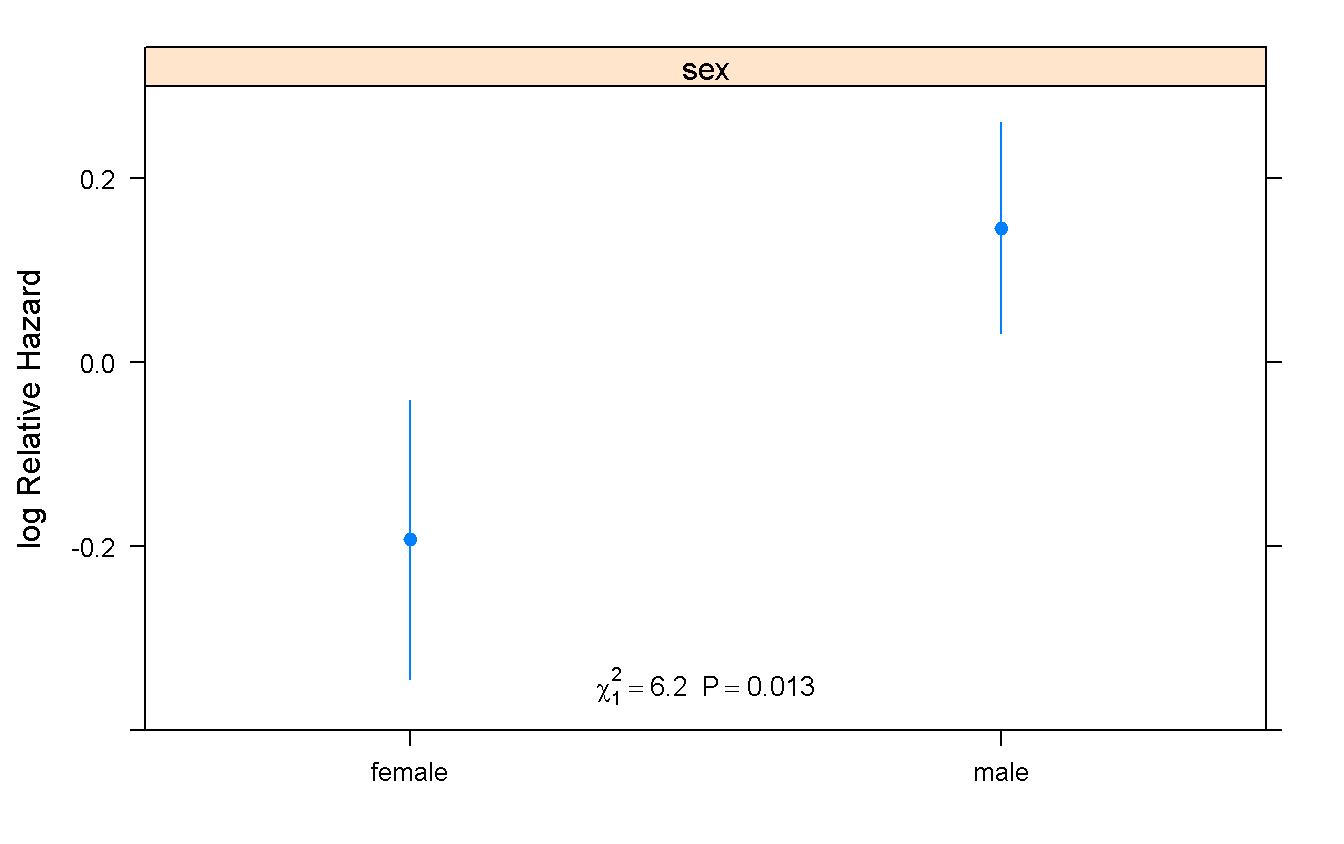
\includegraphics{SuDACDa-notes_files/figure-latex/mgus_survdiff_and_rms-1.pdf}

\section{Non parametric Kaplan-Meier estimation of the survival
function}\label{km1}

\begin{enumerate}
\def\labelenumi{\arabic{enumi}.}
\tightlist
\item
  Let consider a sample of \(n = 500\)
\end{enumerate}

\begin{Shaded}
\begin{Highlighting}[]
\NormalTok{n <-}\StringTok{ }\DecValTok{500}
\end{Highlighting}
\end{Shaded}

\begin{enumerate}
\def\labelenumi{\arabic{enumi}.}
\setcounter{enumi}{1}
\tightlist
\item
  Simulate the dates of entry in the cohort, from January, 2010 to
  January, 2017
\end{enumerate}

\begin{Shaded}
\begin{Highlighting}[]
\NormalTok{n_days <-}\StringTok{ }\FloatTok{365.25} \NormalTok{*}\StringTok{ }\DecValTok{7}              \CommentTok{# Seven years, taking into account bissextiles}
\NormalTok{time_start <-}\StringTok{ }\KeywordTok{runif}\NormalTok{(}\DataTypeTok{n =} \NormalTok{n,}
  \DataTypeTok{min =} \DecValTok{0}\NormalTok{,}
  \DataTypeTok{max =} \NormalTok{n_days}
\NormalTok{) %>%}\StringTok{ }
\StringTok{  }\KeywordTok{as.Date}\NormalTok{(}\DataTypeTok{origin =} \StringTok{'2010-01-01'}\NormalTok{)}
\end{Highlighting}
\end{Shaded}

\begin{enumerate}
\def\labelenumi{\arabic{enumi}.}
\setcounter{enumi}{2}
\tightlist
\item
  Simulate the data-set of death, assuming exponential death times of
  mean \(2\) years
\end{enumerate}

\begin{Shaded}
\begin{Highlighting}[]
\NormalTok{mean_death_time <-}\StringTok{ }\FloatTok{365.25} \NormalTok{*}\StringTok{ }\DecValTok{2}
\NormalTok{death_t         <-}\StringTok{ }\KeywordTok{rexp}\NormalTok{(n, }\DataTypeTok{rate =} \DecValTok{1} \NormalTok{/}\StringTok{ }\NormalTok{mean_death_time)}
\NormalTok{status_no_cens  <-}\StringTok{ }\KeywordTok{rep}\NormalTok{(}\DecValTok{1}\NormalTok{, n)}
\end{Highlighting}
\end{Shaded}

\begin{enumerate}
\def\labelenumi{\arabic{enumi}.}
\setcounter{enumi}{3}
\tightlist
\item
  Let fix the reference date of the analyses of June, 2017
\end{enumerate}

\begin{Shaded}
\begin{Highlighting}[]
\NormalTok{end_date     <-}\StringTok{ }\KeywordTok{as.Date}\NormalTok{(}\StringTok{'2017-06-01'}\NormalTok{)           }\CommentTok{# Fixed date for the end of f-up}
\NormalTok{death_r_cens <-}\StringTok{ }\KeywordTok{pmin}\NormalTok{(death_t, end_date -}\StringTok{ }\NormalTok{time_start)}
\NormalTok{status_cens  <-}\StringTok{ }\NormalTok{status_no_cens -}\StringTok{ }\NormalTok{(death_t ==}\StringTok{ }\NormalTok{death_r_cens)}
\end{Highlighting}
\end{Shaded}

\begin{enumerate}
\def\labelenumi{\arabic{enumi}.}
\setcounter{enumi}{4}
\tightlist
\item
  Estimate the survival function from randomization
\end{enumerate}

\begin{Shaded}
\begin{Highlighting}[]
\KeywordTok{survfit}\NormalTok{(}\KeywordTok{Surv}\NormalTok{(death_r_cens, status_cens) ~}\StringTok{ }\DecValTok{1}\NormalTok{) %>%}\StringTok{ }
\StringTok{  }\KeywordTok{plot}\NormalTok{(}
    \DataTypeTok{conf.int  =} \OtherTok{TRUE}\NormalTok{,}
    \DataTypeTok{mark.time =} \OtherTok{TRUE}\NormalTok{,}
    \DataTypeTok{main      =} \StringTok{'Survival curve from randomization (right censored at 2017-06-01)'}\NormalTok{,}
    \DataTypeTok{col       =} \StringTok{'blue'}\NormalTok{,}
    \DataTypeTok{xlab      =} \StringTok{'Years'}\NormalTok{,}
    \DataTypeTok{xscale    =} \FloatTok{365.25}
\NormalTok{)}
\end{Highlighting}
\end{Shaded}

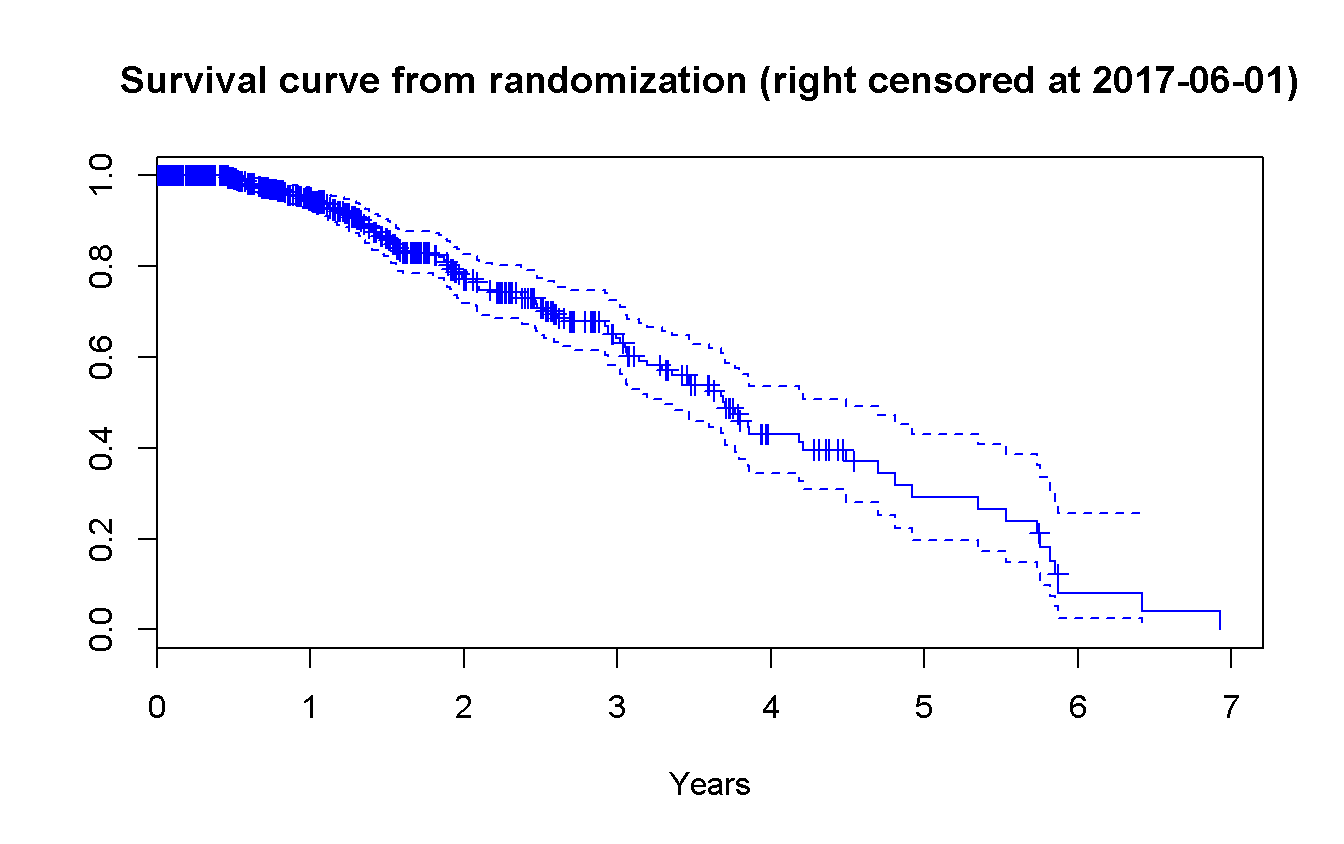
\includegraphics{SuDACDa-notes_files/figure-latex/ex_surv_curves-1.pdf}

\chapter{\texorpdfstring{\emph{Tuesday}: Cox
models}{Tuesday: Cox models}}\label{cox}

\section{Key (operative) concepts}\label{key2}

\begin{enumerate}
\def\labelenumi{\arabic{enumi}.}
\tightlist
\item
  Non-informative censoring assumption!
\end{enumerate}

\begin{quote}
We cannot test for it, but we can be convinced of it
\end{quote}

\begin{enumerate}
\def\labelenumi{\arabic{enumi}.}
\setcounter{enumi}{1}
\tightlist
\item
  Test any covariates for proportional hazard. If fail:
\end{enumerate}

\begin{itemize}
\tightlist
\item
  If \(H_0\) is valid, it is not a problem
\item
  Is it due to outliers?
\item
  Does this variable really need?
\item
  \ldots{} do you really think that proportional of hazard should hold?
  What about shift to a different model?
\end{itemize}

\begin{enumerate}
\def\labelenumi{\arabic{enumi}.}
\setcounter{enumi}{2}
\tightlist
\item
  Test continuous variable for log-linearity. If fail:
\end{enumerate}

\begin{itemize}
\tightlist
\item
  try a transformation of the variable (i.e., log, spline, \ldots{})
\item
  if it is not possible (e.g. \emph{U-shape}) perform a categorization
\end{itemize}

\begin{quote}
When performing categorization do not base it on the p-value: you have
to explain why this choiche is clinically relevant and not statistically
significant!
\end{quote}

\begin{enumerate}
\def\labelenumi{\arabic{enumi}.}
\setcounter{enumi}{3}
\tightlist
\item
  The biggest problem with databases with more observations for each
  patients is not the model but to produce a table with the right
  information in the right position. In particular we need the following
  columns
\end{enumerate}

\begin{itemize}
\tightlist
\item
  id
\item
  start
\item
  end
\item
  event
\item
  covariates\ldots{}
\end{itemize}

\begin{enumerate}
\def\labelenumi{\arabic{enumi}.}
\setcounter{enumi}{4}
\tightlist
\item
  Get results easy to explain to / understand by a clinician!
\end{enumerate}

\section{Basic tests and funtions}\label{test2}

For this part we will use the data \texttt{pbc} (\texttt{?pbc}) from the
package \textbf{survival}.

\begin{quote}
Note: \texttt{data(pbc)} load the \texttt{pbc} data-set and the
\texttt{pbcseq} one, so on one side we do not need to call
\texttt{data(pbcseq)} to load the letter, on the other side
\texttt{data(pbcseq)} will throw an error because to load it we have to
call \texttt{data(pbc)}. (We will use both data-sets.)
\end{quote}

\begin{Shaded}
\begin{Highlighting}[]
\KeywordTok{set.seed}\NormalTok{(}\DecValTok{171003}\NormalTok{)}
\KeywordTok{data}\NormalTok{(pbc)                                                    }\CommentTok{# load the data-set}
\CommentTok{# ?pbc}
\NormalTok{pbc_df <-}\StringTok{ }\KeywordTok{as_tibble}\NormalTok{(pbc)                       }\CommentTok{# create the tibble version of it}
\NormalTok{dd <-}\StringTok{ }\KeywordTok{datadist}\NormalTok{(pbc_df)     }\CommentTok{# store in the dd variable its `datadist()` for _rms_}

\NormalTok{pbc_df                                                       }\CommentTok{# give a look at it}
\end{Highlighting}
\end{Shaded}

\begin{verbatim}
## # A tibble: 418 x 20
##       id  time status   trt      age    sex ascites hepato spiders edema
##    <int> <int>  <int> <int>    <dbl> <fctr>   <int>  <int>   <int> <dbl>
##  1     1   400      2     1 58.76523      f       1      1       1   1.0
##  2     2  4500      0     1 56.44627      f       0      1       1   0.0
##  3     3  1012      2     1 70.07255      m       0      0       0   0.5
##  4     4  1925      2     1 54.74059      f       0      1       1   0.5
##  5     5  1504      1     2 38.10541      f       0      1       1   0.0
##  6     6  2503      2     2 66.25873      f       0      1       0   0.0
##  7     7  1832      0     2 55.53457      f       0      1       0   0.0
##  8     8  2466      2     2 53.05681      f       0      0       0   0.0
##  9     9  2400      2     1 42.50787      f       0      0       1   0.0
## 10    10    51      2     2 70.55989      f       1      0       1   1.0
## # ... with 408 more rows, and 10 more variables: bili <dbl>, chol <int>,
## #   albumin <dbl>, copper <int>, alk.phos <dbl>, ast <dbl>, trig <int>,
## #   platelet <int>, protime <dbl>, stage <int>
\end{verbatim}

\begin{Shaded}
\begin{Highlighting}[]
\KeywordTok{describe}\NormalTok{(pbc_df)                                 }\CommentTok{# and whatch at some statistics}
\end{Highlighting}
\end{Shaded}

\begin{verbatim}
## pbc_df 
## 
##  20  Variables      418  Observations
## ---------------------------------------------------------------------------
## id 
##        n  missing distinct     Info     Mean      Gmd      .05      .10 
##      418        0      418        1    209.5    139.7    21.85    42.70 
##      .25      .50      .75      .90      .95 
##   105.25   209.50   313.75   376.30   397.15 
## 
## lowest :   1   2   3   4   5, highest: 414 415 416 417 418
## ---------------------------------------------------------------------------
## time 
##        n  missing distinct     Info     Mean      Gmd      .05      .10 
##      418        0      399        1     1918     1253    245.1    606.8 
##      .25      .50      .75      .90      .95 
##   1092.8   1730.0   2613.5   3524.2   4040.6 
## 
## lowest :   41   43   51   71   77, highest: 4500 4509 4523 4556 4795
## ---------------------------------------------------------------------------
## status 
##        n  missing distinct     Info     Mean      Gmd 
##      418        0        3    0.772   0.8301   0.9699 
##                             
## Value          0     1     2
## Frequency    232    25   161
## Proportion 0.555 0.060 0.385
## ---------------------------------------------------------------------------
## trt 
##        n  missing distinct     Info     Mean      Gmd 
##      312      106        2     0.75    1.494   0.5015 
##                       
## Value          1     2
## Frequency    158   154
## Proportion 0.506 0.494
## ---------------------------------------------------------------------------
## age 
##        n  missing distinct     Info     Mean      Gmd      .05      .10 
##      418        0      344        1    50.74    11.96    33.84    36.37 
##      .25      .50      .75      .90      .95 
##    42.83    51.00    58.24    64.30    67.92 
## 
## lowest : 26.27789 28.88433 29.55510 30.27515 30.57358
## highest: 74.52430 75.00068 75.01164 76.70910 78.43943
## ---------------------------------------------------------------------------
## sex 
##        n  missing distinct 
##      418        0        2 
##                       
## Value          m     f
## Frequency     44   374
## Proportion 0.105 0.895
## ---------------------------------------------------------------------------
## ascites 
##        n  missing distinct     Info      Sum     Mean      Gmd 
##      312      106        2    0.213       24  0.07692   0.1425 
## 
## ---------------------------------------------------------------------------
## hepato 
##        n  missing distinct     Info      Sum     Mean      Gmd 
##      312      106        2     0.75      160   0.5128   0.5013 
## 
## ---------------------------------------------------------------------------
## spiders 
##        n  missing distinct     Info      Sum     Mean      Gmd 
##      312      106        2    0.616       90   0.2885   0.4118 
## 
## ---------------------------------------------------------------------------
## edema 
##        n  missing distinct     Info     Mean      Gmd 
##      418        0        3    0.391   0.1005   0.1756 
##                             
## Value        0.0   0.5   1.0
## Frequency    354    44    20
## Proportion 0.847 0.105 0.048
## ---------------------------------------------------------------------------
## bili 
##        n  missing distinct     Info     Mean      Gmd      .05      .10 
##      418        0       98    0.998    3.221    3.742     0.50     0.60 
##      .25      .50      .75      .90      .95 
##     0.80     1.40     3.40     8.03    14.00 
## 
## lowest :  0.3  0.4  0.5  0.6  0.7, highest: 21.6 22.5 24.5 25.5 28.0
## ---------------------------------------------------------------------------
## chol 
##        n  missing distinct     Info     Mean      Gmd      .05      .10 
##      284      134      201        1    369.5    194.5    188.4    213.6 
##      .25      .50      .75      .90      .95 
##    249.5    309.5    400.0    560.8    674.0 
## 
## lowest :  120  127  132  149  151, highest: 1336 1480 1600 1712 1775
## ---------------------------------------------------------------------------
## albumin 
##        n  missing distinct     Info     Mean      Gmd      .05      .10 
##      418        0      154        1    3.497    0.473    2.750    2.967 
##      .25      .50      .75      .90      .95 
##    3.243    3.530    3.770    4.010    4.141 
## 
## lowest : 1.96 2.10 2.23 2.27 2.31, highest: 4.30 4.38 4.40 4.52 4.64
## ---------------------------------------------------------------------------
## copper 
##        n  missing distinct     Info     Mean      Gmd      .05      .10 
##      310      108      158        1    97.65    83.16    17.45    24.00 
##      .25      .50      .75      .90      .95 
##    41.25    73.00   123.00   208.10   249.20 
## 
## lowest :   4   9  10  11  12, highest: 412 444 464 558 588
## ---------------------------------------------------------------------------
## alk.phos 
##        n  missing distinct     Info     Mean      Gmd      .05      .10 
##      312      106      295        1     1983     1760    599.6    663.0 
##      .25      .50      .75      .90      .95 
##    871.5   1259.0   1980.0   3826.4   6669.9 
## 
## lowest :   289.0   310.0   369.0   377.0   414.0
## highest: 11046.6 11320.2 11552.0 12258.8 13862.4
## ---------------------------------------------------------------------------
## ast 
##        n  missing distinct     Info     Mean      Gmd      .05      .10 
##      312      106      179        1    122.6    60.45    54.25    60.45 
##      .25      .50      .75      .90      .95 
##    80.60   114.70   151.90   196.47   219.25 
## 
## lowest :  26.35  28.38  41.85  43.40  45.00, highest: 288.00 299.15 328.60 338.00 457.25
## ---------------------------------------------------------------------------
## trig 
##        n  missing distinct     Info     Mean      Gmd      .05      .10 
##      282      136      146        1    124.7    64.07    56.00    63.10 
##      .25      .50      .75      .90      .95 
##    84.25   108.00   151.00   195.00   230.95 
## 
## lowest :  33  44  46  49  50, highest: 319 322 382 432 598
## ---------------------------------------------------------------------------
## platelet 
##        n  missing distinct     Info     Mean      Gmd      .05      .10 
##      407       11      243        1      257    109.7    114.9    138.2 
##      .25      .50      .75      .90      .95 
##    188.5    251.0    318.0    386.2    430.0 
## 
## lowest :  62  70  71  76  79, highest: 517 518 539 563 721
## ---------------------------------------------------------------------------
## protime 
##        n  missing distinct     Info     Mean      Gmd      .05      .10 
##      416        2       48    0.998    10.73    1.029     9.60     9.80 
##      .25      .50      .75      .90      .95 
##    10.00    10.60    11.10    12.00    12.45 
## 
## lowest :  9.0  9.1  9.2  9.3  9.4, highest: 13.8 14.1 15.2 17.1 18.0
## ---------------------------------------------------------------------------
## stage 
##        n  missing distinct     Info     Mean      Gmd 
##      412        6        4    0.893    3.024   0.9519 
##                                   
## Value          1     2     3     4
## Frequency     21    92   155   144
## Proportion 0.051 0.223 0.376 0.350
## ---------------------------------------------------------------------------
\end{verbatim}

\subsection{Impact of sex on death
\{sex2\}}\label{impact-of-sex-on-death-sex2}

First of all we have to ask to our self, and to the clinicians, some
questions:

\begin{enumerate}
\def\labelenumi{\arabic{enumi}.}
\item
  There are non-informative censoring? Yes, because there is a final
  data-independent date (i.e.~July, 1986). This is completely
  non-informative with regards to the patients. So we can suspect a
  non-informative censoring and start investigations using Cox model.
\item
  What we have to do with the transplant? I.e., \texttt{event} has three
  levels: censored, transplant, dead; how we have to consider
  transplanted patients? In this case, clinicians answered that the
  transplant status is completely random! So, we can believe that it is
  a non-informative censoring.\footnote{In reality this is not really
    true because who stay better is on the top of the list!}
\end{enumerate}

Moreover we have to consider, before to start, that \texttt{sex} is a
categorical variable, so we have to check (only) the proportionality of
the hazards.

\begin{Shaded}
\begin{Highlighting}[]
\CommentTok{# Using _survival_ (Cox model for proportional hazard against sex)}
\NormalTok{cox_sex <-}\StringTok{ }\KeywordTok{coxph}\NormalTok{(}\KeywordTok{Surv}\NormalTok{(time, status ==}\StringTok{ }\DecValTok{2}\NormalTok{) ~}\StringTok{ }\NormalTok{sex,}
  \DataTypeTok{data =} \NormalTok{pbc_df}
\NormalTok{)}

\KeywordTok{cox.zph}\NormalTok{(cox_sex)                           }\CommentTok{# test for proportionality of hazards}
\end{Highlighting}
\end{Shaded}

\begin{verbatim}
##          rho chisq     p
## sexf -0.0563 0.502 0.479
\end{verbatim}

\begin{Shaded}
\begin{Highlighting}[]
\KeywordTok{cox.zph}\NormalTok{(cox_sex) %>%}\StringTok{ }
\StringTok{  }\KeywordTok{plot}\NormalTok{(}
    \DataTypeTok{main =} \StringTok{'Graph of the scaled Schoenfeld residuals for sex, along with a smooth curve'}\NormalTok{,}
    \DataTypeTok{col =} \StringTok{'blue'}
\NormalTok{)}
\end{Highlighting}
\end{Shaded}

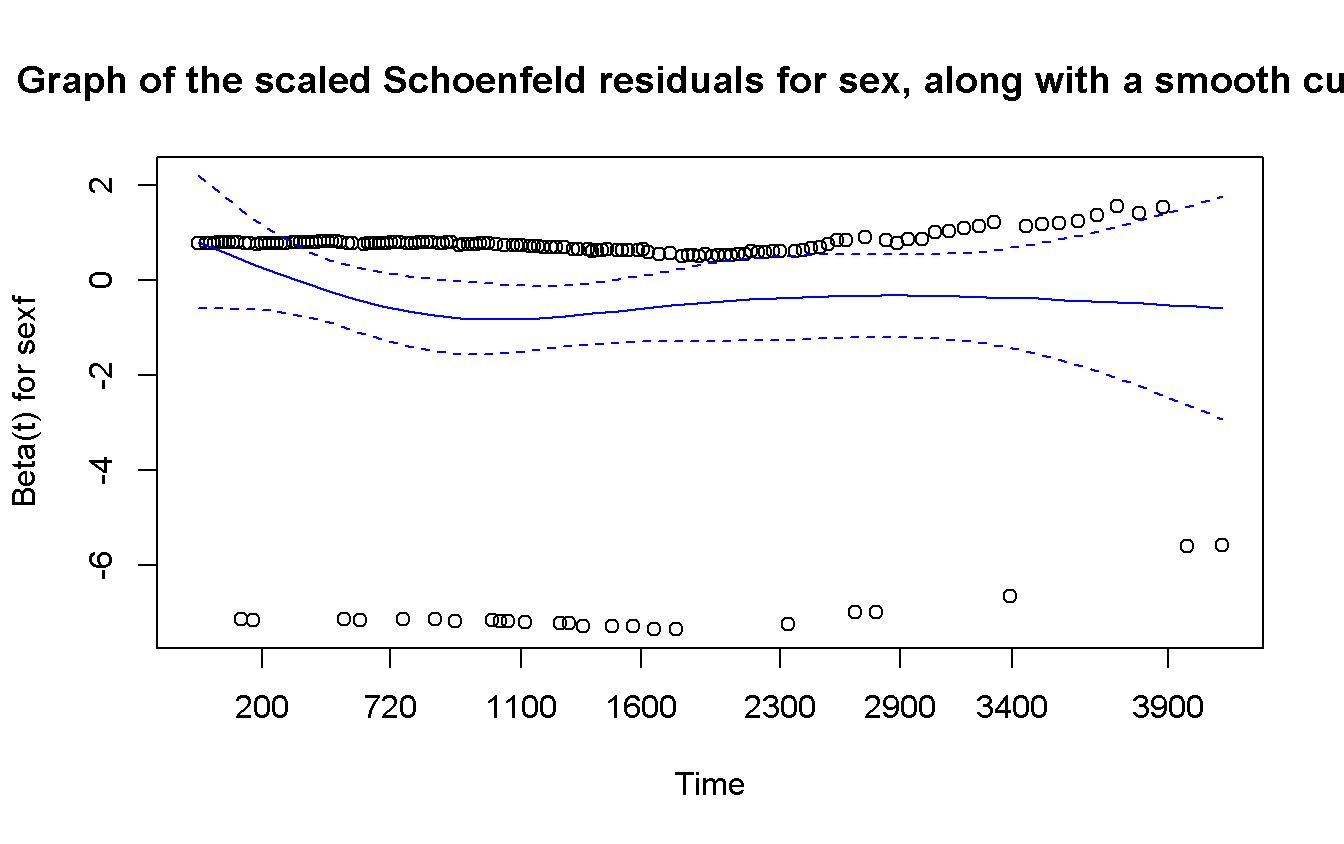
\includegraphics{SuDACDa-notes_files/figure-latex/unnamed-chunk-3-1.pdf}

The proportional hazard assumption is not invalidate so we can continue
with the analyses.

\begin{Shaded}
\begin{Highlighting}[]
\KeywordTok{summary}\NormalTok{(cox_sex)}
\end{Highlighting}
\end{Shaded}

\begin{verbatim}
## Call:
## coxph(formula = Surv(time, status == 2) ~ sex, data = pbc_df)
## 
##   n= 418, number of events= 161 
## 
##         coef exp(coef) se(coef)      z Pr(>|z|)  
## sexf -0.3809    0.6833   0.2221 -1.714   0.0864 .
## ---
## Signif. codes:  0 '***' 0.001 '**' 0.01 '*' 0.05 '.' 0.1 ' ' 1
## 
##      exp(coef) exp(-coef) lower .95 upper .95
## sexf    0.6833      1.464    0.4421     1.056
## 
## Concordance= 0.518  (se = 0.013 )
## Rsquare= 0.006   (max possible= 0.985 )
## Likelihood ratio test= 2.69  on 1 df,   p=0.101
## Wald test            = 2.94  on 1 df,   p=0.08645
## Score (logrank) test = 2.97  on 1 df,   p=0.08459
\end{verbatim}

The effect of sex, viewed as hazard ration, say that if you are a female
it seems that you have a lower risk to die, but it is not significant
(i.e., \(p\)-value \(> 0.05\) and CI include \(1\)).

\begin{quote}
Anyone have the same risk, 1, to die\ldots{} What the hazard ration say
is that if at the begin of a day you are alive, if you a re a woman you
have 32\% less probability to die before the end of the day respect a
men.
\end{quote}

\begin{Shaded}
\begin{Highlighting}[]
\CommentTok{# Using rms}
\NormalTok{rms_sex <-}\StringTok{ }\KeywordTok{cph}\NormalTok{(}\KeywordTok{Surv}\NormalTok{(time, status ==}\StringTok{ }\DecValTok{2}\NormalTok{) ~}\StringTok{ }\NormalTok{sex,}
  \DataTypeTok{data =} \NormalTok{pbc_df,}
  \DataTypeTok{x    =} \OtherTok{TRUE}\NormalTok{,                    }\CommentTok{# to compute cox.zph, we need to store x and y}
  \DataTypeTok{y    =} \OtherTok{TRUE}
\NormalTok{)}

\KeywordTok{cox.zph}\NormalTok{(rms_sex)}
\end{Highlighting}
\end{Shaded}

\begin{verbatim}
##           rho chisq     p
## sex=f -0.0563 0.501 0.479
\end{verbatim}

\begin{Shaded}
\begin{Highlighting}[]
\KeywordTok{cox.zph}\NormalTok{(rms_sex) %>%}\StringTok{ }
\StringTok{  }\KeywordTok{plot}\NormalTok{(}\DataTypeTok{col =} \StringTok{'green'}\NormalTok{)                       }\CommentTok{# exactly the same results as before!}
\end{Highlighting}
\end{Shaded}

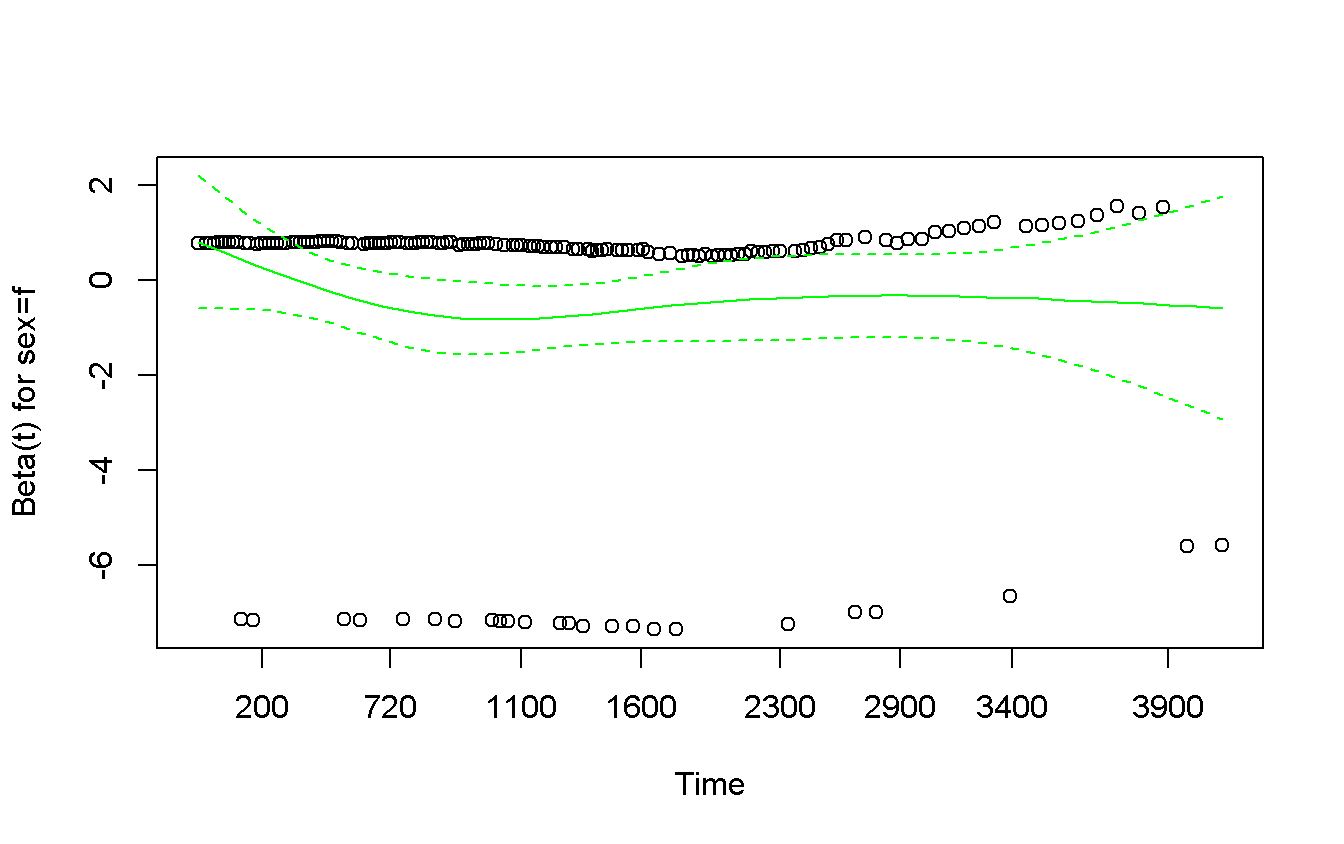
\includegraphics{SuDACDa-notes_files/figure-latex/unnamed-chunk-5-1.pdf}

\begin{Shaded}
\begin{Highlighting}[]
\KeywordTok{summary}\NormalTok{(rms_sex)       }\CommentTok{# a cleaner and more informative output, note Low and High}
\end{Highlighting}
\end{Shaded}

\begin{verbatim}
##              Effects              Response : Surv(time, status == 2) 
## 
##  Factor        Low High Diff. Effect  S.E.    Lower 0.95 Upper 0.95
##  sex - m:f     2   1    NA    0.38206 0.22205 -0.053149  0.81727   
##   Hazard Ratio 2   1    NA    1.46530      NA  0.948240  2.26430
\end{verbatim}

\subsection{Impact of age on death}\label{age2}

\begin{itemize}
\tightlist
\item
  we have to check for the proportional HR
\item
  It is continuous variable, we have to check the the log-linearity too
\end{itemize}

\begin{Shaded}
\begin{Highlighting}[]
\CommentTok{# Using survival}
\NormalTok{cox_age <-}\StringTok{ }\KeywordTok{coxph}\NormalTok{(}\KeywordTok{Surv}\NormalTok{(time, status ==}\StringTok{ }\DecValTok{2}\NormalTok{) ~}\StringTok{ }\NormalTok{age,}
  \DataTypeTok{data =} \NormalTok{pbc_df}
\NormalTok{)}

\KeywordTok{cox.zph}\NormalTok{(cox_age)}
\end{Highlighting}
\end{Shaded}

\begin{verbatim}
##         rho chisq    p
## age -0.0304 0.139 0.71
\end{verbatim}

\begin{Shaded}
\begin{Highlighting}[]
\KeywordTok{cox.zph}\NormalTok{(cox_age) %>%}
\StringTok{  }\KeywordTok{plot}\NormalTok{(}\DataTypeTok{col =} \StringTok{'blue'}\NormalTok{)}
\end{Highlighting}
\end{Shaded}

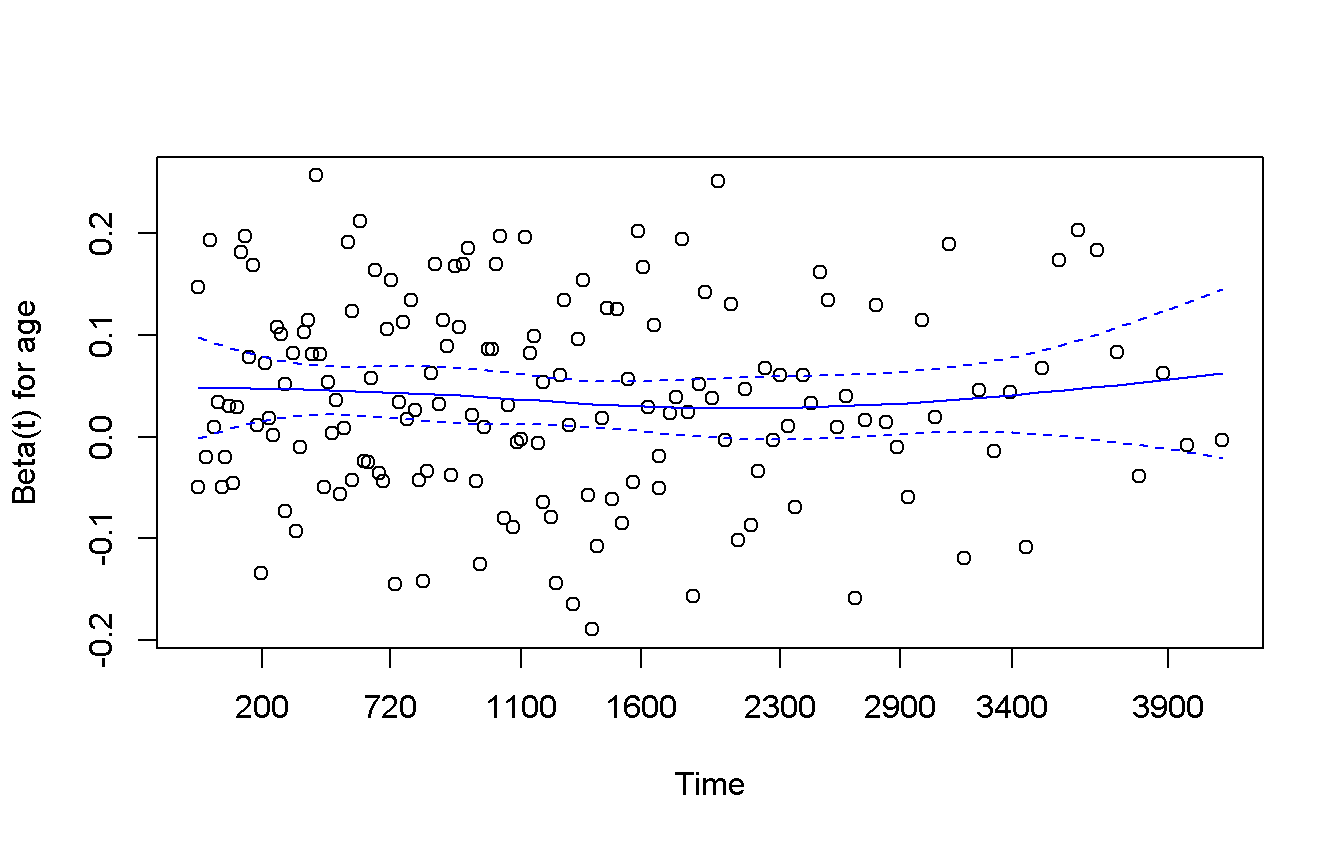
\includegraphics{SuDACDa-notes_files/figure-latex/unnamed-chunk-6-1.pdf}

The proportional hazard hypothesis is not invalidated

\begin{Shaded}
\begin{Highlighting}[]
\CommentTok{# [Note: unfortunately the option `noprint` of the funciton `rcspline.plot`}
\CommentTok{#  does not work and the space-waste list of all the coefficients and relative}
\CommentTok{#  SE will be printed all the time. Sorry, we are working for a solution.]}
\KeywordTok{rcspline.plot}\NormalTok{(}
  \DataTypeTok{x       =} \NormalTok{pbc_df$age,}
  \DataTypeTok{y       =} \NormalTok{pbc_df$time,}
  \DataTypeTok{event   =} \NormalTok{pbc_df$status ==}\StringTok{ }\DecValTok{2}\NormalTok{,}
  \DataTypeTok{nk      =} \DecValTok{3}\NormalTok{,                   }\CommentTok{# default are 5 knots, too mutch for this model}
\CommentTok{#  model   = 'cox',          # If event is present, model is assumed to be "cox"}
  \DataTypeTok{xlab    =} \StringTok{'Age'}\NormalTok{,}
  \DataTypeTok{statloc =} \StringTok{'ll'}
\NormalTok{)}
\end{Highlighting}
\end{Shaded}

\begin{verbatim}
##           x             
##  0.05307827 -0.01469916 
## [1] -873.4721 -860.6518
\end{verbatim}

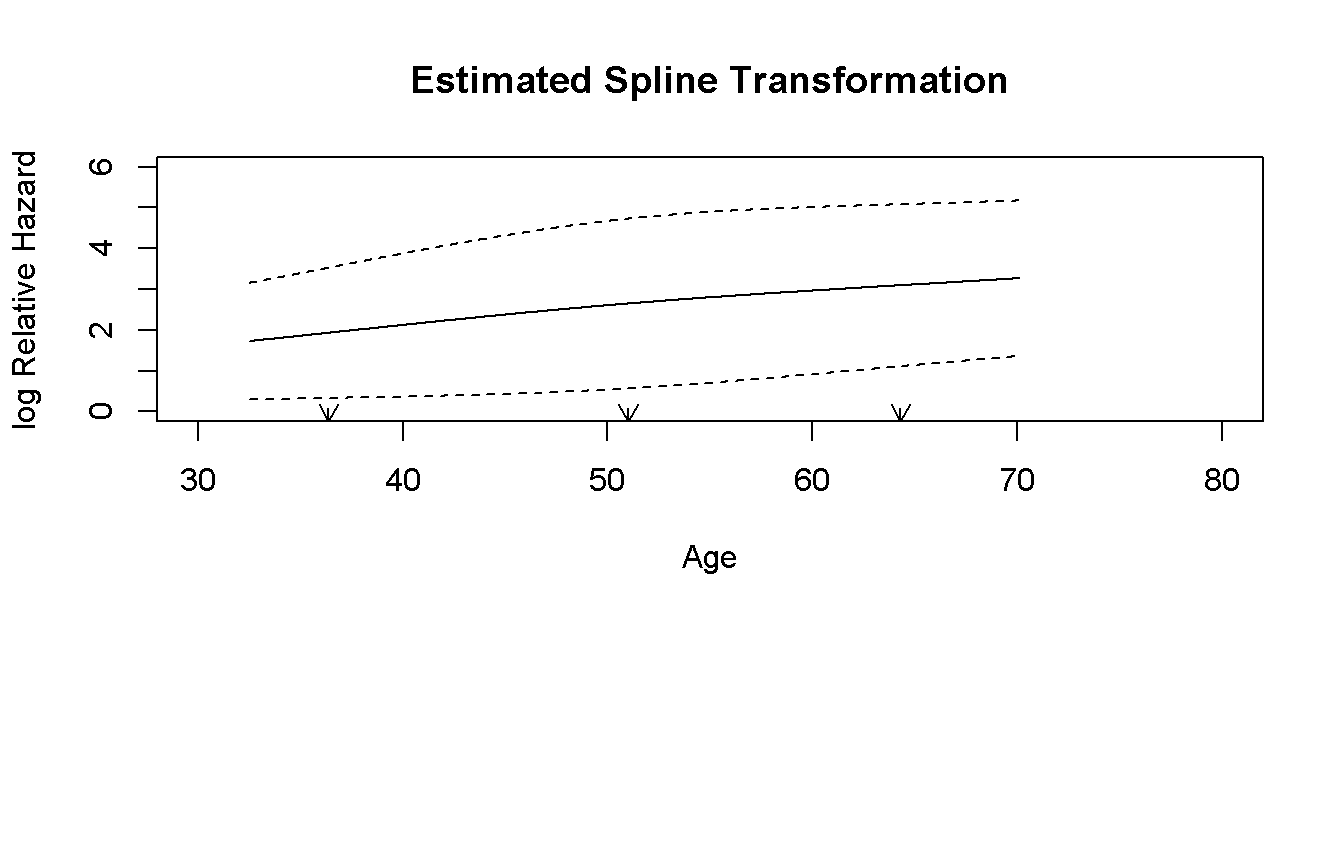
\includegraphics{SuDACDa-notes_files/figure-latex/unnamed-chunk-7-1.pdf}

\begin{verbatim}
## 
## cbind(xe, lower, upper)
## 
##              xe                   
##   [1,] 32.50350 0.2957928 3.154667
##   [2,] 32.56624 0.2963637 3.160756
##   [3,] 32.62898 0.2969347 3.166845
##   [4,] 32.69172 0.2975056 3.172934
##   [5,] 32.75446 0.2980765 3.179024
##   [6,] 32.81720 0.2986475 3.185113
##   [7,] 32.87994 0.2992184 3.191202
##   [8,] 32.94268 0.2997894 3.197291
##   [9,] 33.00542 0.3003603 3.203381
##  [10,] 33.06815 0.3009313 3.209470
##  [11,] 33.13089 0.3015022 3.215559
##  [12,] 33.19363 0.3020732 3.221648
##  [13,] 33.25637 0.3026441 3.227737
##  [14,] 33.31911 0.3032151 3.233827
##  [15,] 33.38185 0.3037860 3.239916
##  [16,] 33.44459 0.3043570 3.246005
##  [17,] 33.50733 0.3049279 3.252094
##  [18,] 33.57007 0.3054989 3.258184
##  [19,] 33.63281 0.3060698 3.264273
##  [20,] 33.69555 0.3066407 3.270362
##  [21,] 33.75828 0.3072117 3.276451
##  [22,] 33.82102 0.3077826 3.282540
##  [23,] 33.88376 0.3083536 3.288630
##  [24,] 33.94650 0.3089245 3.294719
##  [25,] 34.00924 0.3094955 3.300808
##  [26,] 34.07198 0.3100664 3.306897
##  [27,] 34.13472 0.3106374 3.312986
##  [28,] 34.19746 0.3112083 3.319076
##  [29,] 34.26020 0.3117793 3.325165
##  [30,] 34.32294 0.3123502 3.331254
##  [31,] 34.38567 0.3129212 3.337343
##  [32,] 34.44841 0.3134921 3.343433
##  [33,] 34.51115 0.3140631 3.349522
##  [34,] 34.57389 0.3146340 3.355611
##  [35,] 34.63663 0.3152049 3.361700
##  [36,] 34.69937 0.3157759 3.367789
##  [37,] 34.76211 0.3163468 3.373879
##  [38,] 34.82485 0.3169178 3.379968
##  [39,] 34.88759 0.3174887 3.386057
##  [40,] 34.95033 0.3180597 3.392146
##  [41,] 35.01307 0.3186306 3.398236
##  [42,] 35.07580 0.3192016 3.404325
##  [43,] 35.13854 0.3197725 3.410414
##  [44,] 35.20128 0.3203435 3.416503
##  [45,] 35.26402 0.3209144 3.422592
##  [46,] 35.32676 0.3214854 3.428682
##  [47,] 35.38950 0.3220563 3.434771
##  [48,] 35.45224 0.3226273 3.440860
##  [49,] 35.51498 0.3231982 3.446949
##  [50,] 35.57772 0.3237691 3.453038
##  [51,] 35.64046 0.3243401 3.459128
##  [52,] 35.70320 0.3249110 3.465217
##  [53,] 35.76593 0.3254820 3.471306
##  [54,] 35.82867 0.3260529 3.477395
##  [55,] 35.89141 0.3266239 3.483485
##  [56,] 35.95415 0.3271948 3.489574
##  [57,] 36.01689 0.3277658 3.495663
##  [58,] 36.07963 0.3283367 3.501752
##  [59,] 36.14237 0.3289077 3.507841
##  [60,] 36.20511 0.3294786 3.513931
##  [61,] 36.26785 0.3300496 3.520020
##  [62,] 36.33059 0.3306205 3.526109
##  [63,] 36.39333 0.3311915 3.532198
##  [64,] 36.45606 0.3317624 3.538287
##  [65,] 36.51880 0.3323335 3.544376
##  [66,] 36.58154 0.3329046 3.550465
##  [67,] 36.64428 0.3334759 3.556554
##  [68,] 36.70702 0.3340475 3.562642
##  [69,] 36.76976 0.3346192 3.568729
##  [70,] 36.83250 0.3351913 3.574816
##  [71,] 36.89524 0.3357638 3.580902
##  [72,] 36.95798 0.3363367 3.586987
##  [73,] 37.02072 0.3369100 3.593071
##  [74,] 37.08346 0.3374838 3.599154
##  [75,] 37.14619 0.3380582 3.605236
##  [76,] 37.20893 0.3386332 3.611316
##  [77,] 37.27167 0.3392089 3.617395
##  [78,] 37.33441 0.3397852 3.623473
##  [79,] 37.39715 0.3403623 3.629549
##  [80,] 37.45989 0.3409402 3.635623
##  [81,] 37.52263 0.3415189 3.641696
##  [82,] 37.58537 0.3420985 3.647766
##  [83,] 37.64811 0.3426791 3.653835
##  [84,] 37.71085 0.3432607 3.659901
##  [85,] 37.77359 0.3438433 3.665966
##  [86,] 37.83632 0.3444270 3.672028
##  [87,] 37.89906 0.3450118 3.678087
##  [88,] 37.96180 0.3455978 3.684144
##  [89,] 38.02454 0.3461850 3.690198
##  [90,] 38.08728 0.3467736 3.696249
##  [91,] 38.15002 0.3473634 3.702298
##  [92,] 38.21276 0.3479547 3.708344
##  [93,] 38.27550 0.3485474 3.714386
##  [94,] 38.33824 0.3491415 3.720426
##  [95,] 38.40098 0.3497372 3.726462
##  [96,] 38.46372 0.3503344 3.732494
##  [97,] 38.52645 0.3509333 3.738524
##  [98,] 38.58919 0.3515339 3.744549
##  [99,] 38.65193 0.3521361 3.750571
## [100,] 38.71467 0.3527402 3.756589
## [101,] 38.77741 0.3533460 3.762604
## [102,] 38.84015 0.3539537 3.768614
## [103,] 38.90289 0.3545634 3.774620
## [104,] 38.96563 0.3551750 3.780622
## [105,] 39.02837 0.3557886 3.786619
## [106,] 39.09111 0.3564043 3.792612
## [107,] 39.15385 0.3570221 3.798601
## [108,] 39.21658 0.3576420 3.804585
## [109,] 39.27932 0.3582641 3.810564
## [110,] 39.34206 0.3588886 3.816539
## [111,] 39.40480 0.3595153 3.822508
## [112,] 39.46754 0.3601443 3.828473
## [113,] 39.53028 0.3607758 3.834432
## [114,] 39.59302 0.3614097 3.840386
## [115,] 39.65576 0.3620461 3.846334
## [116,] 39.71850 0.3626851 3.852277
## [117,] 39.78124 0.3633266 3.858215
## [118,] 39.84397 0.3639708 3.864147
## [119,] 39.90671 0.3646177 3.870073
## [120,] 39.96945 0.3652673 3.875993
## [121,] 40.03219 0.3659197 3.881907
## [122,] 40.09493 0.3665750 3.887816
## [123,] 40.15767 0.3672331 3.893717
## [124,] 40.22041 0.3678942 3.899613
## [125,] 40.28315 0.3685582 3.905502
## [126,] 40.34589 0.3692253 3.911385
## [127,] 40.40863 0.3698955 3.917261
## [128,] 40.47137 0.3705688 3.923130
## [129,] 40.53410 0.3712452 3.928993
## [130,] 40.59684 0.3719249 3.934848
## [131,] 40.65958 0.3726079 3.940697
## [132,] 40.72232 0.3732942 3.946538
## [133,] 40.78506 0.3739838 3.952373
## [134,] 40.84780 0.3746769 3.958199
## [135,] 40.91054 0.3753735 3.964019
## [136,] 40.97328 0.3760735 3.969831
## [137,] 41.03602 0.3767771 3.975635
## [138,] 41.09876 0.3774844 3.981431
## [139,] 41.16150 0.3781953 3.987220
## [140,] 41.22423 0.3789099 3.993000
## [141,] 41.28697 0.3796282 3.998773
## [142,] 41.34971 0.3803504 4.004537
## [143,] 41.41245 0.3810764 4.010293
## [144,] 41.47519 0.3818063 4.016041
## [145,] 41.53793 0.3825402 4.021780
## [146,] 41.60067 0.3832780 4.027510
## [147,] 41.66341 0.3840200 4.033232
## [148,] 41.72615 0.3847660 4.038945
## [149,] 41.78889 0.3855161 4.044649
## [150,] 41.85163 0.3862704 4.050344
## [151,] 41.91436 0.3870290 4.056030
## [152,] 41.97710 0.3877919 4.061707
## [153,] 42.03984 0.3885591 4.067375
## [154,] 42.10258 0.3893307 4.073033
## [155,] 42.16532 0.3901067 4.078681
## [156,] 42.22806 0.3908872 4.084320
## [157,] 42.29080 0.3916722 4.089949
## [158,] 42.35354 0.3924618 4.095568
## [159,] 42.41628 0.3932560 4.101178
## [160,] 42.47902 0.3940549 4.106777
## [161,] 42.54176 0.3948585 4.112366
## [162,] 42.60449 0.3956669 4.117945
## [163,] 42.66723 0.3964801 4.123513
## [164,] 42.72997 0.3972981 4.129071
## [165,] 42.79271 0.3981211 4.134619
## [166,] 42.85545 0.3989490 4.140155
## [167,] 42.91819 0.3997820 4.145681
## [168,] 42.98093 0.4006200 4.151197
## [169,] 43.04367 0.4014630 4.156701
## [170,] 43.10641 0.4023113 4.162194
## [171,] 43.16915 0.4031647 4.167676
## [172,] 43.23189 0.4040234 4.173146
## [173,] 43.29462 0.4048874 4.178605
## [174,] 43.35736 0.4057567 4.184053
## [175,] 43.42010 0.4066314 4.189489
## [176,] 43.48284 0.4075116 4.194913
## [177,] 43.54558 0.4083972 4.200326
## [178,] 43.60832 0.4092883 4.205726
## [179,] 43.67106 0.4101851 4.211115
## [180,] 43.73380 0.4110874 4.216491
## [181,] 43.79654 0.4119955 4.221856
## [182,] 43.85928 0.4129092 4.227207
## [183,] 43.92202 0.4138288 4.232547
## [184,] 43.98475 0.4147541 4.237874
## [185,] 44.04749 0.4156853 4.243188
## [186,] 44.11023 0.4166224 4.248490
## [187,] 44.17297 0.4175655 4.253778
## [188,] 44.23571 0.4185146 4.259054
## [189,] 44.29845 0.4194698 4.264317
## [190,] 44.36119 0.4204310 4.269566
## [191,] 44.42393 0.4213984 4.274803
## [192,] 44.48667 0.4223720 4.280026
## [193,] 44.54941 0.4233518 4.285235
## [194,] 44.61215 0.4243379 4.290431
## [195,] 44.67488 0.4253304 4.295613
## [196,] 44.73762 0.4263292 4.300782
## [197,] 44.80036 0.4273344 4.305936
## [198,] 44.86310 0.4283462 4.311077
## [199,] 44.92584 0.4293645 4.316203
## [200,] 44.98858 0.4303893 4.321315
## [201,] 45.05132 0.4314207 4.326414
## [202,] 45.11406 0.4324589 4.331497
## [203,] 45.17680 0.4335037 4.336566
## [204,] 45.23954 0.4345553 4.341621
## [205,] 45.30227 0.4356137 4.346661
## [206,] 45.36501 0.4366789 4.351686
## [207,] 45.42775 0.4377511 4.356696
## [208,] 45.49049 0.4388301 4.361691
## [209,] 45.55323 0.4399162 4.366671
## [210,] 45.61597 0.4410093 4.371636
## [211,] 45.67871 0.4421095 4.376585
## [212,] 45.74145 0.4432169 4.381520
## [213,] 45.80419 0.4443314 4.386438
## [214,] 45.86693 0.4454531 4.391341
## [215,] 45.92967 0.4465821 4.396228
## [216,] 45.99240 0.4477185 4.401100
## [217,] 46.05514 0.4488621 4.405955
## [218,] 46.11788 0.4500132 4.410795
## [219,] 46.18062 0.4511718 4.415618
## [220,] 46.24336 0.4523378 4.420425
## [221,] 46.30610 0.4535114 4.425216
## [222,] 46.36884 0.4546926 4.429990
## [223,] 46.43158 0.4558814 4.434748
## [224,] 46.49432 0.4570779 4.439489
## [225,] 46.55706 0.4582822 4.444214
## [226,] 46.61980 0.4594942 4.448921
## [227,] 46.68253 0.4607140 4.453612
## [228,] 46.74527 0.4619417 4.458286
## [229,] 46.80801 0.4631773 4.462942
## [230,] 46.87075 0.4644209 4.467581
## [231,] 46.93349 0.4656725 4.472203
## [232,] 46.99623 0.4669321 4.476808
## [233,] 47.05897 0.4681998 4.481395
## [234,] 47.12171 0.4694757 4.485964
## [235,] 47.18445 0.4707597 4.490515
## [236,] 47.24719 0.4720520 4.495049
## [237,] 47.30993 0.4733526 4.499565
## [238,] 47.37266 0.4746614 4.504062
## [239,] 47.43540 0.4759787 4.508542
## [240,] 47.49814 0.4773043 4.513003
## [241,] 47.56088 0.4786384 4.517446
## [242,] 47.62362 0.4799810 4.521870
## [243,] 47.68636 0.4813322 4.526276
## [244,] 47.74910 0.4826919 4.530663
## [245,] 47.81184 0.4840603 4.535032
## [246,] 47.87458 0.4854373 4.539381
## [247,] 47.93732 0.4868231 4.543712
## [248,] 48.00006 0.4882177 4.548023
## [249,] 48.06279 0.4896210 4.552316
## [250,] 48.12553 0.4910332 4.556589
## [251,] 48.18827 0.4924543 4.560842
## [252,] 48.25101 0.4938844 4.565077
## [253,] 48.31375 0.4953234 4.569291
## [254,] 48.37649 0.4967715 4.573487
## [255,] 48.43923 0.4982287 4.577662
## [256,] 48.50197 0.4996949 4.581817
## [257,] 48.56471 0.5011704 4.585953
## [258,] 48.62745 0.5026550 4.590068
## [259,] 48.69019 0.5041489 4.594163
## [260,] 48.75292 0.5056521 4.598238
## [261,] 48.81566 0.5071646 4.602293
## [262,] 48.87840 0.5086866 4.606327
## [263,] 48.94114 0.5102179 4.610341
## [264,] 49.00388 0.5117587 4.614334
## [265,] 49.06662 0.5133090 4.618306
## [266,] 49.12936 0.5148689 4.622258
## [267,] 49.19210 0.5164383 4.626188
## [268,] 49.25484 0.5180174 4.630097
## [269,] 49.31758 0.5196062 4.633986
## [270,] 49.38032 0.5212047 4.637853
## [271,] 49.44305 0.5228130 4.641698
## [272,] 49.50579 0.5244311 4.645523
## [273,] 49.56853 0.5260590 4.649325
## [274,] 49.63127 0.5276969 4.653106
## [275,] 49.69401 0.5293446 4.656866
## [276,] 49.75675 0.5310024 4.660603
## [277,] 49.81949 0.5326702 4.664319
## [278,] 49.88223 0.5343480 4.668012
## [279,] 49.94497 0.5360359 4.671683
## [280,] 50.00771 0.5377340 4.675333
## [281,] 50.07045 0.5394423 4.678959
## [282,] 50.13318 0.5411608 4.682564
## [283,] 50.19592 0.5428895 4.686146
## [284,] 50.25866 0.5446286 4.689705
## [285,] 50.32140 0.5463781 4.693242
## [286,] 50.38414 0.5481379 4.696755
## [287,] 50.44688 0.5499081 4.700246
## [288,] 50.50962 0.5516889 4.703714
## [289,] 50.57236 0.5534801 4.707159
## [290,] 50.63510 0.5552819 4.710580
## [291,] 50.69784 0.5570943 4.713979
## [292,] 50.76058 0.5589174 4.717354
## [293,] 50.82331 0.5607511 4.720705
## [294,] 50.88605 0.5625955 4.724033
## [295,] 50.94879 0.5644507 4.727337
## [296,] 51.01153 0.5663167 4.730617
## [297,] 51.07427 0.5681935 4.733874
## [298,] 51.13701 0.5700810 4.737107
## [299,] 51.19975 0.5719793 4.740316
## [300,] 51.26249 0.5738881 4.743502
## [301,] 51.32523 0.5758076 4.746665
## [302,] 51.38797 0.5777376 4.749804
## [303,] 51.45070 0.5796780 4.752920
## [304,] 51.51344 0.5816288 4.756013
## [305,] 51.57618 0.5835900 4.759084
## [306,] 51.63892 0.5855614 4.762131
## [307,] 51.70166 0.5875430 4.765156
## [308,] 51.76440 0.5895348 4.768159
## [309,] 51.82714 0.5915367 4.771139
## [310,] 51.88988 0.5935486 4.774097
## [311,] 51.95262 0.5955705 4.777033
## [312,] 52.01536 0.5976023 4.779947
## [313,] 52.07810 0.5996439 4.782839
## [314,] 52.14083 0.6016953 4.785709
## [315,] 52.20357 0.6037564 4.788558
## [316,] 52.26631 0.6058272 4.791385
## [317,] 52.32905 0.6079076 4.794191
## [318,] 52.39179 0.6099975 4.796975
## [319,] 52.45453 0.6120970 4.799738
## [320,] 52.51727 0.6142058 4.802481
## [321,] 52.58001 0.6163240 4.805202
## [322,] 52.64275 0.6184515 4.807903
## [323,] 52.70549 0.6205882 4.810583
## [324,] 52.76823 0.6227341 4.813242
## [325,] 52.83096 0.6248891 4.815881
## [326,] 52.89370 0.6270531 4.818500
## [327,] 52.95644 0.6292262 4.821099
## [328,] 53.01918 0.6314081 4.823677
## [329,] 53.08192 0.6335990 4.826236
## [330,] 53.14466 0.6357986 4.828775
## [331,] 53.20740 0.6380070 4.831294
## [332,] 53.27014 0.6402241 4.833794
## [333,] 53.33288 0.6424498 4.836274
## [334,] 53.39562 0.6446841 4.838735
## [335,] 53.45836 0.6469268 4.841177
## [336,] 53.52109 0.6491780 4.843600
## [337,] 53.58383 0.6514376 4.846004
## [338,] 53.64657 0.6537055 4.848389
## [339,] 53.70931 0.6559816 4.850755
## [340,] 53.77205 0.6582660 4.853103
## [341,] 53.83479 0.6605584 4.855432
## [342,] 53.89753 0.6628590 4.857744
## [343,] 53.96027 0.6651675 4.860036
## [344,] 54.02301 0.6674840 4.862311
## [345,] 54.08575 0.6698084 4.864568
## [346,] 54.14849 0.6721406 4.866807
## [347,] 54.21122 0.6744806 4.869028
## [348,] 54.27396 0.6768283 4.871232
## [349,] 54.33670 0.6791836 4.873418
## [350,] 54.39944 0.6815465 4.875587
## [351,] 54.46218 0.6839169 4.877739
## [352,] 54.52492 0.6862948 4.879874
## [353,] 54.58766 0.6886801 4.881991
## [354,] 54.65040 0.6910727 4.884092
## [355,] 54.71314 0.6934726 4.886176
## [356,] 54.77588 0.6958797 4.888244
## [357,] 54.83862 0.6982939 4.890295
## [358,] 54.90135 0.7007153 4.892329
## [359,] 54.96409 0.7031436 4.894348
## [360,] 55.02683 0.7055790 4.896350
## [361,] 55.08957 0.7080212 4.898337
## [362,] 55.15231 0.7104703 4.900307
## [363,] 55.21505 0.7129262 4.902262
## [364,] 55.27779 0.7153888 4.904201
## [365,] 55.34053 0.7178581 4.906125
## [366,] 55.40327 0.7203340 4.908033
## [367,] 55.46601 0.7228164 4.909926
## [368,] 55.52875 0.7253053 4.911804
## [369,] 55.59148 0.7278006 4.913667
## [370,] 55.65422 0.7303023 4.915515
## [371,] 55.71696 0.7328102 4.917348
## [372,] 55.77970 0.7353244 4.919166
## [373,] 55.84244 0.7378448 4.920970
## [374,] 55.90518 0.7403713 4.922760
## [375,] 55.96792 0.7429039 4.924536
## [376,] 56.03066 0.7454424 4.926297
## [377,] 56.09340 0.7479869 4.928044
## [378,] 56.15614 0.7505372 4.929777
## [379,] 56.21888 0.7530934 4.931497
## [380,] 56.28161 0.7556553 4.933203
## [381,] 56.34435 0.7582229 4.934895
## [382,] 56.40709 0.7607961 4.936574
## [383,] 56.46983 0.7633749 4.938240
## [384,] 56.53257 0.7659592 4.939892
## [385,] 56.59531 0.7685489 4.941532
## [386,] 56.65805 0.7711441 4.943158
## [387,] 56.72079 0.7737445 4.944772
## [388,] 56.78353 0.7763502 4.946373
## [389,] 56.84627 0.7789612 4.947961
## [390,] 56.90900 0.7815772 4.949537
## [391,] 56.97174 0.7841984 4.951101
## [392,] 57.03448 0.7868246 4.952652
## [393,] 57.09722 0.7894557 4.954191
## [394,] 57.15996 0.7920917 4.955719
## [395,] 57.22270 0.7947326 4.957234
## [396,] 57.28544 0.7973783 4.958738
## [397,] 57.34818 0.8000287 4.960231
## [398,] 57.41092 0.8026837 4.961711
## [399,] 57.47366 0.8053434 4.963181
## [400,] 57.53640 0.8080076 4.964639
## [401,] 57.59913 0.8106763 4.966086
## [402,] 57.66187 0.8133494 4.967522
## [403,] 57.72461 0.8160268 4.968948
## [404,] 57.78735 0.8187086 4.970362
## [405,] 57.85009 0.8213946 4.971766
## [406,] 57.91283 0.8240848 4.973160
## [407,] 57.97557 0.8267791 4.974543
## [408,] 58.03831 0.8294775 4.975915
## [409,] 58.10105 0.8321799 4.977278
## [410,] 58.16379 0.8348862 4.978631
## [411,] 58.22653 0.8375964 4.979974
## [412,] 58.28926 0.8403105 4.981307
## [413,] 58.35200 0.8430283 4.982630
## [414,] 58.41474 0.8457498 4.983944
## [415,] 58.47748 0.8484750 4.985248
## [416,] 58.54022 0.8512037 4.986543
## [417,] 58.60296 0.8539360 4.987829
## [418,] 58.66570 0.8566718 4.989106
## [419,] 58.72844 0.8594110 4.990374
## [420,] 58.79118 0.8621535 4.991633
## [421,] 58.85392 0.8648993 4.992883
## [422,] 58.91666 0.8676484 4.994125
## [423,] 58.97939 0.8704006 4.995359
## [424,] 59.04213 0.8731559 4.996584
## [425,] 59.10487 0.8759143 4.997801
## [426,] 59.16761 0.8786758 4.999009
## [427,] 59.23035 0.8814401 5.000210
## [428,] 59.29309 0.8842074 5.001403
## [429,] 59.35583 0.8869774 5.002588
## [430,] 59.41857 0.8897503 5.003766
## [431,] 59.48131 0.8925258 5.004936
## [432,] 59.54405 0.8953040 5.006099
## [433,] 59.60679 0.8980848 5.007255
## [434,] 59.66952 0.9008681 5.008403
## [435,] 59.73226 0.9036539 5.009544
## [436,] 59.79500 0.9064422 5.010679
## [437,] 59.85774 0.9092328 5.011806
## [438,] 59.92048 0.9120256 5.012928
## [439,] 59.98322 0.9148208 5.014042
## [440,] 60.04596 0.9176181 5.015150
## [441,] 60.10870 0.9204176 5.016252
## [442,] 60.17144 0.9232191 5.017348
## [443,] 60.23418 0.9260227 5.018437
## [444,] 60.29692 0.9288282 5.019521
## [445,] 60.35965 0.9316357 5.020598
## [446,] 60.42239 0.9344450 5.021671
## [447,] 60.48513 0.9372560 5.022737
## [448,] 60.54787 0.9400688 5.023798
## [449,] 60.61061 0.9428833 5.024854
## [450,] 60.67335 0.9456994 5.025904
## [451,] 60.73609 0.9485171 5.026949
## [452,] 60.79883 0.9513363 5.027990
## [453,] 60.86157 0.9541569 5.029025
## [454,] 60.92431 0.9569790 5.030056
## [455,] 60.98705 0.9598023 5.031082
## [456,] 61.04978 0.9626270 5.032103
## [457,] 61.11252 0.9654529 5.033120
## [458,] 61.17526 0.9682799 5.034133
## [459,] 61.23800 0.9711081 5.035142
## [460,] 61.30074 0.9739374 5.036146
## [461,] 61.36348 0.9767676 5.037147
## [462,] 61.42622 0.9795988 5.038143
## [463,] 61.48896 0.9824309 5.039136
## [464,] 61.55170 0.9852638 5.040126
## [465,] 61.61444 0.9880976 5.041112
## [466,] 61.67718 0.9909320 5.042094
## [467,] 61.73991 0.9937671 5.043074
## [468,] 61.80265 0.9966029 5.044050
## [469,] 61.86539 0.9994392 5.045023
## [470,] 61.92813 1.0022761 5.045993
## [471,] 61.99087 1.0051134 5.046961
## [472,] 62.05361 1.0079511 5.047926
## [473,] 62.11635 1.0107891 5.048888
## [474,] 62.17909 1.0136275 5.049848
## [475,] 62.24183 1.0164661 5.050805
## [476,] 62.30457 1.0193049 5.051761
## [477,] 62.36730 1.0221438 5.052714
## [478,] 62.43004 1.0249828 5.053665
## [479,] 62.49278 1.0278218 5.054615
## [480,] 62.55552 1.0306608 5.055562
## [481,] 62.61826 1.0334998 5.056508
## [482,] 62.68100 1.0363386 5.057453
## [483,] 62.74374 1.0391772 5.058396
## [484,] 62.80648 1.0420156 5.059338
## [485,] 62.86922 1.0448537 5.060278
## [486,] 62.93196 1.0476915 5.061218
## [487,] 62.99470 1.0505289 5.062156
## [488,] 63.05743 1.0533658 5.063094
## [489,] 63.12017 1.0562023 5.064031
## [490,] 63.18291 1.0590381 5.064967
## [491,] 63.24565 1.0618734 5.065903
## [492,] 63.30839 1.0647081 5.066839
## [493,] 63.37113 1.0675420 5.067774
## [494,] 63.43387 1.0703752 5.068709
## [495,] 63.49661 1.0732076 5.069644
## [496,] 63.55935 1.0760391 5.070579
## [497,] 63.62209 1.0788698 5.071515
## [498,] 63.68483 1.0816994 5.072450
## [499,] 63.74756 1.0845281 5.073386
## [500,] 63.81030 1.0873557 5.074323
## [501,] 63.87304 1.0901822 5.075260
## [502,] 63.93578 1.0930076 5.076198
## [503,] 63.99852 1.0958317 5.077136
## [504,] 64.06126 1.0986546 5.078076
## [505,] 64.12400 1.1014762 5.079017
## [506,] 64.18674 1.1042964 5.079958
## [507,] 64.24948 1.1071152 5.080902
## [508,] 64.31222 1.1099326 5.081846
## [509,] 64.37496 1.1127485 5.082792
## [510,] 64.43769 1.1155629 5.083740
## [511,] 64.50043 1.1183757 5.084689
## [512,] 64.56317 1.1211871 5.085639
## [513,] 64.62591 1.1239970 5.086592
## [514,] 64.68865 1.1268054 5.087545
## [515,] 64.75139 1.1296122 5.088500
## [516,] 64.81413 1.1324176 5.089457
## [517,] 64.87687 1.1352214 5.090415
## [518,] 64.93961 1.1380237 5.091375
## [519,] 65.00235 1.1408245 5.092336
## [520,] 65.06509 1.1436238 5.093298
## [521,] 65.12782 1.1464216 5.094262
## [522,] 65.19056 1.1492178 5.095228
## [523,] 65.25330 1.1520125 5.096195
## [524,] 65.31604 1.1548057 5.097164
## [525,] 65.37878 1.1575974 5.098134
## [526,] 65.44152 1.1603875 5.099106
## [527,] 65.50426 1.1631761 5.100080
## [528,] 65.56700 1.1659631 5.101055
## [529,] 65.62974 1.1687486 5.102031
## [530,] 65.69248 1.1715326 5.103009
## [531,] 65.75522 1.1743150 5.103988
## [532,] 65.81795 1.1770959 5.104969
## [533,] 65.88069 1.1798753 5.105952
## [534,] 65.94343 1.1826531 5.106936
## [535,] 66.00617 1.1854293 5.107922
## [536,] 66.06891 1.1882040 5.108909
## [537,] 66.13165 1.1909771 5.109898
## [538,] 66.19439 1.1937487 5.110888
## [539,] 66.25713 1.1965187 5.111880
## [540,] 66.31987 1.1992872 5.112874
## [541,] 66.38261 1.2020541 5.113869
## [542,] 66.44535 1.2048194 5.114865
## [543,] 66.50808 1.2075831 5.115864
## [544,] 66.57082 1.2103453 5.116863
## [545,] 66.63356 1.2131059 5.117865
## [546,] 66.69630 1.2158650 5.118868
## [547,] 66.75904 1.2186224 5.119872
## [548,] 66.82178 1.2213783 5.120878
## [549,] 66.88452 1.2241326 5.121886
## [550,] 66.94726 1.2268853 5.122895
## [551,] 67.01000 1.2296365 5.123906
## [552,] 67.07274 1.2323860 5.124918
## [553,] 67.13548 1.2351340 5.125932
## [554,] 67.19821 1.2378803 5.126948
## [555,] 67.26095 1.2406251 5.127965
## [556,] 67.32369 1.2433683 5.128984
## [557,] 67.38643 1.2461099 5.130004
## [558,] 67.44917 1.2488499 5.131026
## [559,] 67.51191 1.2515882 5.132050
## [560,] 67.57465 1.2543250 5.133075
## [561,] 67.63739 1.2570602 5.134101
## [562,] 67.70013 1.2597937 5.135130
## [563,] 67.76287 1.2625257 5.136160
## [564,] 67.82560 1.2652560 5.137191
## [565,] 67.88834 1.2679847 5.138225
## [566,] 67.95108 1.2707118 5.139260
## [567,] 68.01382 1.2734373 5.140296
## [568,] 68.07656 1.2761612 5.141334
## [569,] 68.13930 1.2788834 5.142374
## [570,] 68.20204 1.2816040 5.143415
## [571,] 68.26478 1.2843230 5.144458
## [572,] 68.32752 1.2870404 5.145503
## [573,] 68.39026 1.2897561 5.146549
## [574,] 68.45300 1.2924702 5.147597
## [575,] 68.51573 1.2951827 5.148646
## [576,] 68.57847 1.2978935 5.149697
## [577,] 68.64121 1.3006026 5.150750
## [578,] 68.70395 1.3033102 5.151804
## [579,] 68.76669 1.3060161 5.152860
## [580,] 68.82943 1.3087203 5.153918
## [581,] 68.89217 1.3114229 5.154978
## [582,] 68.95491 1.3141239 5.156039
## [583,] 69.01765 1.3168231 5.157101
## [584,] 69.08039 1.3195208 5.158165
## [585,] 69.14313 1.3222168 5.159231
## [586,] 69.20586 1.3249111 5.160299
## [587,] 69.26860 1.3276037 5.161368
## [588,] 69.33134 1.3302947 5.162439
## [589,] 69.39408 1.3329841 5.163512
## [590,] 69.45682 1.3356717 5.164586
## [591,] 69.51956 1.3383577 5.165662
## [592,] 69.58230 1.3410420 5.166740
## [593,] 69.64504 1.3437247 5.167819
## [594,] 69.70778 1.3464056 5.168900
## [595,] 69.77052 1.3490849 5.169983
## [596,] 69.83326 1.3517625 5.171067
## [597,] 69.89599 1.3544385 5.172153
## [598,] 69.95873 1.3571127 5.173241
## [599,] 70.02147 1.3597853 5.174330
## [600,] 70.08421 1.3624561 5.175421
\end{verbatim}

The log-linearity is not invalidated

\begin{quote}
Note: sometimes you \emph{know} the answer for log-linearity (for any
reason), in those cases do not test for it!! (It is not very powerful so
for small sample sizes it never reject it)
\end{quote}

\begin{Shaded}
\begin{Highlighting}[]
\KeywordTok{summary}\NormalTok{(cox_age)}
\end{Highlighting}
\end{Shaded}

\begin{verbatim}
## Call:
## coxph(formula = Surv(time, status == 2) ~ age, data = pbc_df)
## 
##   n= 418, number of events= 161 
## 
##         coef exp(coef) se(coef)     z Pr(>|z|)    
## age 0.039185  1.039963 0.007847 4.994 5.92e-07 ***
## ---
## Signif. codes:  0 '***' 0.001 '**' 0.01 '*' 0.05 '.' 0.1 ' ' 1
## 
##     exp(coef) exp(-coef) lower .95 upper .95
## age      1.04     0.9616     1.024     1.056
## 
## Concordance= 0.616  (se = 0.025 )
## Rsquare= 0.058   (max possible= 0.985 )
## Likelihood ratio test= 25.19  on 1 df,   p=5.205e-07
## Wald test            = 24.94  on 1 df,   p=5.922e-07
## Score (logrank) test = 25.3  on 1 df,   p=4.918e-07
\end{verbatim}

The effect is significant but too low to understand, so we can change
the ``measure of time'' to expand it.

\begin{Shaded}
\begin{Highlighting}[]
\KeywordTok{coxph}\NormalTok{(}\KeywordTok{Surv}\NormalTok{(time, status ==}\StringTok{ }\DecValTok{2}\NormalTok{) ~}\StringTok{ }\KeywordTok{I}\NormalTok{(age /}\StringTok{ }\DecValTok{10}\NormalTok{),          }\CommentTok{# consider 10 years as one}
  \DataTypeTok{data =} \NormalTok{pbc_df}
\NormalTok{) %>%}
\StringTok{  }\NormalTok{summary}
\end{Highlighting}
\end{Shaded}

\begin{verbatim}
## Call:
## coxph(formula = Surv(time, status == 2) ~ I(age/10), data = pbc_df)
## 
##   n= 418, number of events= 161 
## 
##              coef exp(coef) se(coef)     z Pr(>|z|)    
## I(age/10) 0.39185   1.47972  0.07847 4.994 5.92e-07 ***
## ---
## Signif. codes:  0 '***' 0.001 '**' 0.01 '*' 0.05 '.' 0.1 ' ' 1
## 
##           exp(coef) exp(-coef) lower .95 upper .95
## I(age/10)      1.48     0.6758     1.269     1.726
## 
## Concordance= 0.616  (se = 0.025 )
## Rsquare= 0.058   (max possible= 0.985 )
## Likelihood ratio test= 25.19  on 1 df,   p=5.205e-07
## Wald test            = 24.94  on 1 df,   p=5.922e-07
## Score (logrank) test = 25.3  on 1 df,   p=4.918e-07
\end{verbatim}

Here, the effect is increased, but we have to pay attention the an
increment of ``one'', here, corresponds to an increment of ten years!

\begin{Shaded}
\begin{Highlighting}[]
\CommentTok{# Using rms}
\NormalTok{rms_age <-}\StringTok{ }\KeywordTok{cph}\NormalTok{(}\KeywordTok{Surv}\NormalTok{(time, status ==}\StringTok{ }\DecValTok{2}\NormalTok{) ~}\StringTok{ }\NormalTok{age,}
  \DataTypeTok{data =} \NormalTok{pbc_df,}
  \DataTypeTok{x    =} \OtherTok{TRUE}\NormalTok{,                    }\CommentTok{# to compute cox.zph, we need to store x and y}
  \DataTypeTok{y    =} \OtherTok{TRUE}
\NormalTok{)}

\KeywordTok{Predict}\NormalTok{(rms_age) %>%}
\StringTok{  }\NormalTok{plot}
\end{Highlighting}
\end{Shaded}

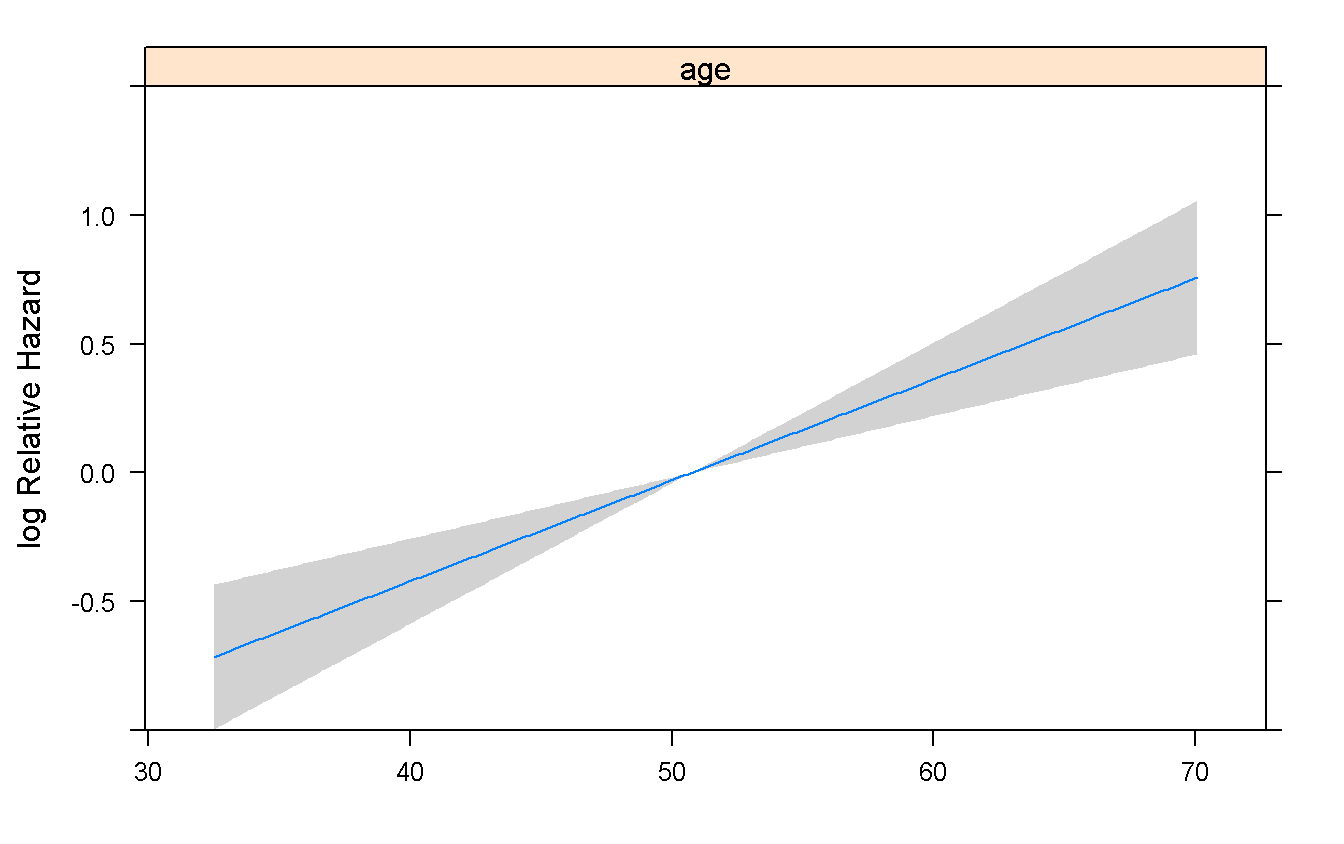
\includegraphics{SuDACDa-notes_files/figure-latex/unnamed-chunk-10-1.pdf}

\begin{Shaded}
\begin{Highlighting}[]
\KeywordTok{summary}\NormalTok{(rms_age)  }\CommentTok{# _rms_ show effects from the Lower to the Higher limit of IQR}
\end{Highlighting}
\end{Shaded}

\begin{verbatim}
##              Effects              Response : Surv(time, status == 2) 
## 
##  Factor        Low    High   Diff.  Effect  S.E.    Lower 0.95 Upper 0.95
##  age           42.832 58.241 15.409 0.60379 0.12091 0.36681    0.84076   
##   Hazard Ratio 42.832 58.241 15.409 1.82900      NA 1.44310    2.31810
\end{verbatim}

\begin{Shaded}
\begin{Highlighting}[]
                  \CommentTok{# and report the different between them as well as the HR, so}
                  \CommentTok{# we do not need to perform triky transformation which asks}
                  \CommentTok{# for an alterate interpretation of the result}
\end{Highlighting}
\end{Shaded}

In particular, the effect quite doubled in fifteen years.\footnote{Good
  example in which only the clinicians know if it is an effect
  clinically relevant (deciding it \textbf{before} the analyses) or not}.

\subsection{\texorpdfstring{Impact of aspartate aminotransferase
(\texttt{ast}) on
death}{Impact of aspartate aminotransferase (ast) on death}}\label{ast2}

\begin{itemize}
\tightlist
\item
  same of age
\end{itemize}

\begin{Shaded}
\begin{Highlighting}[]
\NormalTok{rms_ast <-}\StringTok{ }\KeywordTok{cph}\NormalTok{(}\KeywordTok{Surv}\NormalTok{(time, status ==}\StringTok{ }\DecValTok{2}\NormalTok{) ~}\StringTok{ }\NormalTok{ast,}
  \DataTypeTok{data =} \NormalTok{pbc_df,}
  \DataTypeTok{x    =} \OtherTok{TRUE}\NormalTok{,}
  \DataTypeTok{y    =} \OtherTok{TRUE}
\NormalTok{)}

\KeywordTok{cox.zph}\NormalTok{(rms_ast)}
\end{Highlighting}
\end{Shaded}

\begin{verbatim}
##         rho chisq     p
## ast -0.0641 0.274 0.601
\end{verbatim}

\begin{Shaded}
\begin{Highlighting}[]
\KeywordTok{cox.zph}\NormalTok{(rms_ast) %>%}
\StringTok{  }\KeywordTok{plot}\NormalTok{(}\DataTypeTok{col =} \StringTok{'green'}\NormalTok{)}
\end{Highlighting}
\end{Shaded}

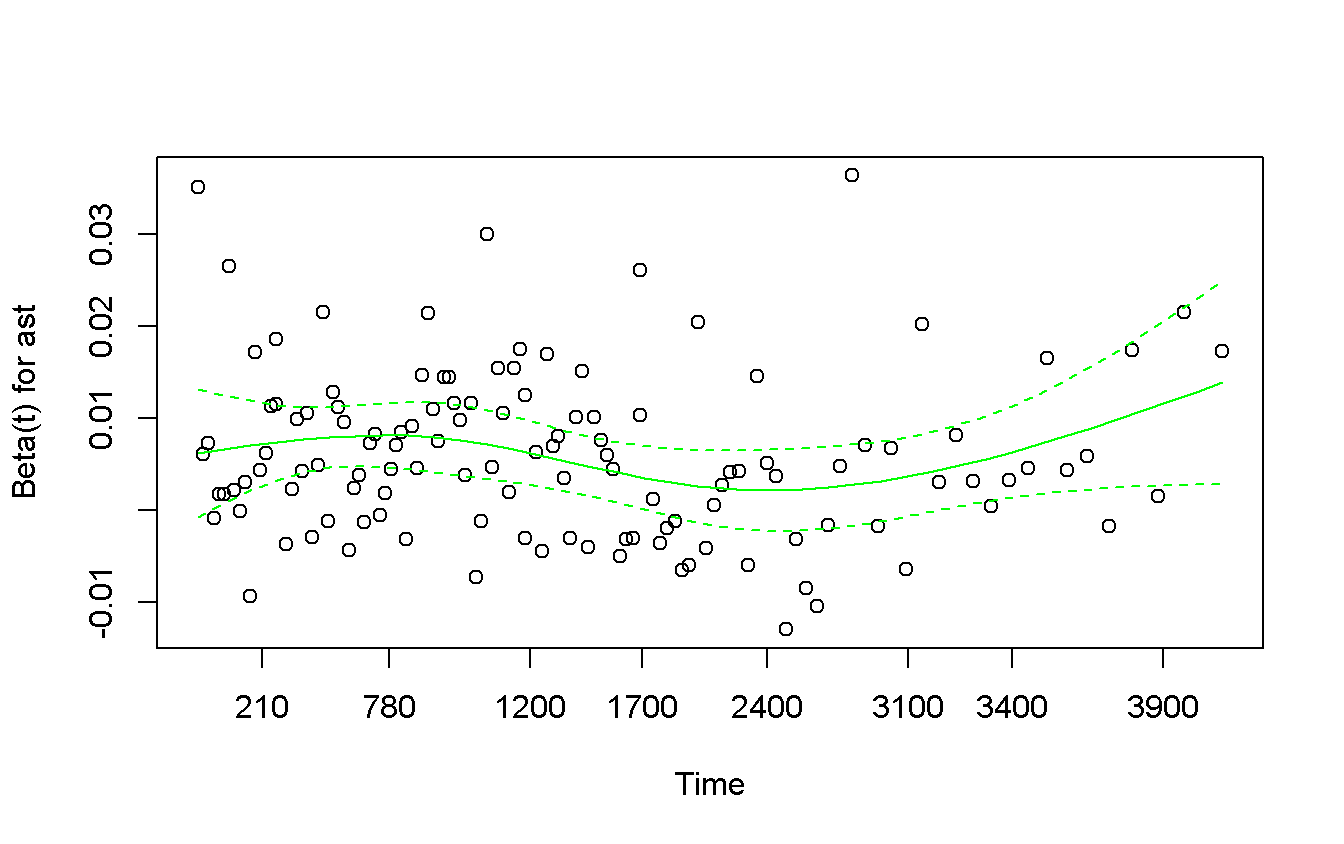
\includegraphics{SuDACDa-notes_files/figure-latex/unnamed-chunk-11-1.pdf}

The proportional hazard assumption is not violated, but by the graph it
seams not that linear. Try to transform it using the \(log()\)
transformation.

\begin{Shaded}
\begin{Highlighting}[]
\NormalTok{log_ast <-}\StringTok{ }\KeywordTok{cph}\NormalTok{(}\KeywordTok{Surv}\NormalTok{(time, status ==}\StringTok{ }\DecValTok{2}\NormalTok{) ~}\StringTok{ }\KeywordTok{log}\NormalTok{(ast),}
  \DataTypeTok{data =} \NormalTok{pbc_df,}
  \DataTypeTok{x    =} \OtherTok{TRUE}\NormalTok{,}
  \DataTypeTok{y    =} \OtherTok{TRUE}
\NormalTok{)}

\KeywordTok{cox.zph}\NormalTok{(log_ast)}
\end{Highlighting}
\end{Shaded}

\begin{verbatim}
##      rho chisq     p
## ast -0.1  1.13 0.289
\end{verbatim}

\begin{Shaded}
\begin{Highlighting}[]
\KeywordTok{cox.zph}\NormalTok{(log_ast) %>%}
\StringTok{  }\KeywordTok{plot}\NormalTok{(}\DataTypeTok{col =} \StringTok{'green'}\NormalTok{)}
\end{Highlighting}
\end{Shaded}

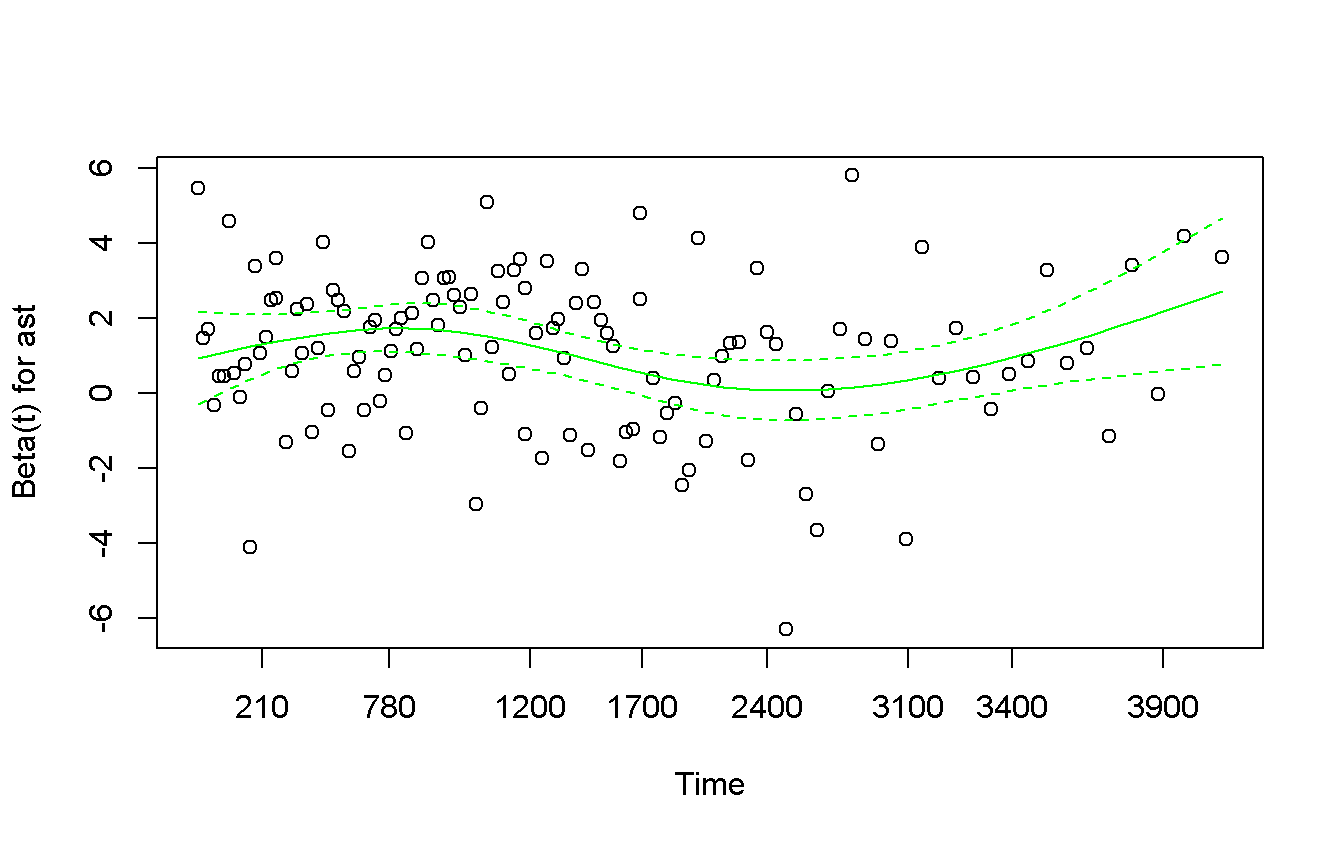
\includegraphics{SuDACDa-notes_files/figure-latex/unnamed-chunk-12-1.pdf}

The situation is not much better\ldots{}but we can say that there exists
a line living in the middle of the band\ldots{}so we are not very happy
but we accept it.

Let's test for log-linearity

\begin{Shaded}
\begin{Highlighting}[]
\KeywordTok{rcspline.plot}\NormalTok{(}
  \DataTypeTok{x       =} \KeywordTok{log}\NormalTok{(pbc_df$ast),}
  \DataTypeTok{y       =} \NormalTok{pbc_df$time,}
  \DataTypeTok{event   =} \NormalTok{pbc_df$status ==}\StringTok{ }\DecValTok{2}\NormalTok{,}
  \DataTypeTok{xlab    =} \StringTok{'ast'}\NormalTok{,}
  \DataTypeTok{statloc =} \StringTok{'ll'}
\NormalTok{)}
\end{Highlighting}
\end{Shaded}

\begin{verbatim}
##           x                                     
## -0.04133714  4.00548693 -7.69016846 -8.96495717 
## [1] -639.9665 -622.2519
\end{verbatim}

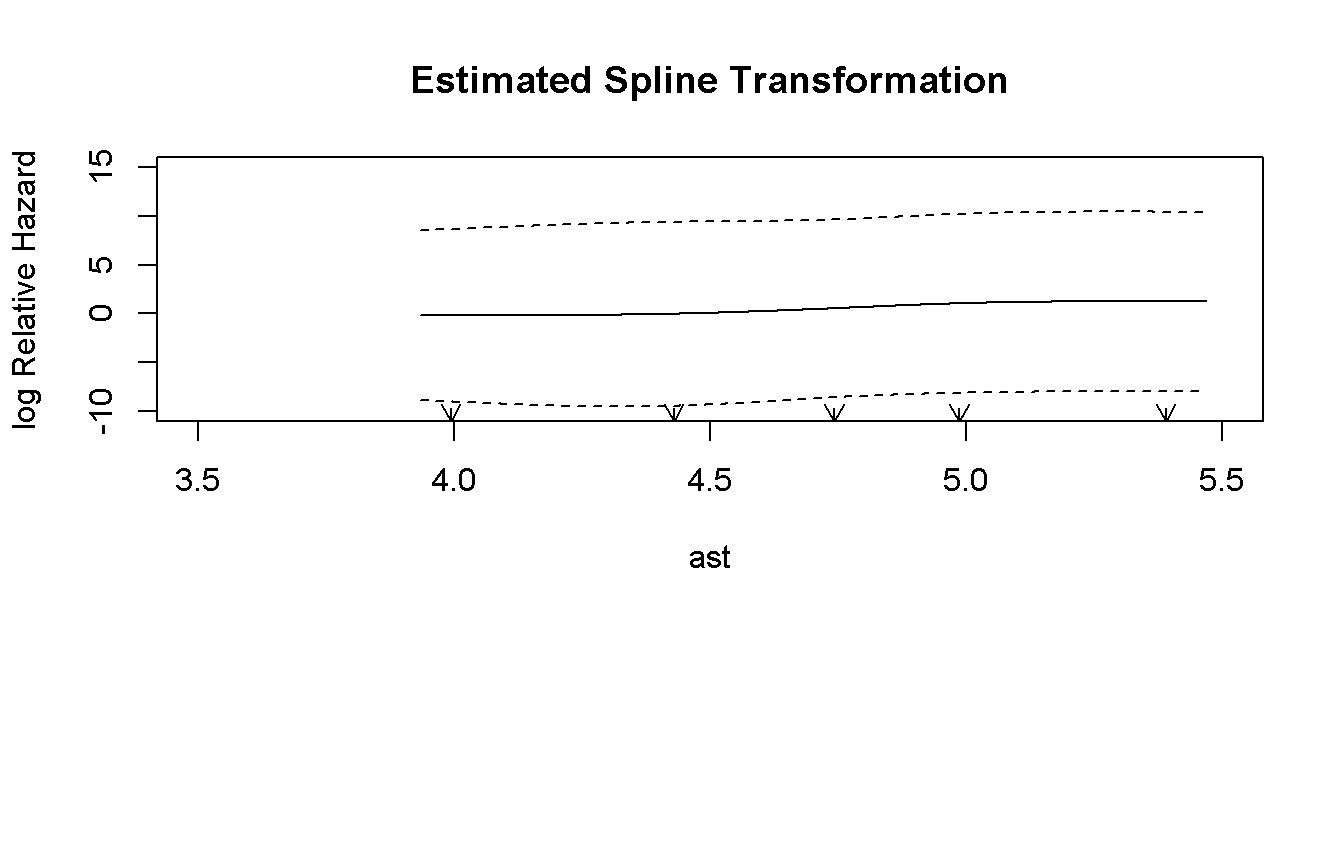
\includegraphics{SuDACDa-notes_files/figure-latex/unnamed-chunk-13-1.pdf}

\begin{verbatim}
## 
## cbind(xe, lower, upper)
## 
##              xe                    
##   [1,] 3.934762 -8.852913  8.527609
##   [2,] 3.937324 -8.858675  8.533160
##   [3,] 3.939885 -8.864438  8.538711
##   [4,] 3.942446 -8.870200  8.544261
##   [5,] 3.945007 -8.875963  8.549812
##   [6,] 3.947568 -8.881725  8.555363
##   [7,] 3.950129 -8.887487  8.560913
##   [8,] 3.952691 -8.893250  8.566464
##   [9,] 3.955252 -8.899012  8.572015
##  [10,] 3.957813 -8.904775  8.577565
##  [11,] 3.960374 -8.910537  8.583116
##  [12,] 3.962935 -8.916300  8.588667
##  [13,] 3.965496 -8.922062  8.594217
##  [14,] 3.968058 -8.927824  8.599768
##  [15,] 3.970619 -8.933587  8.605319
##  [16,] 3.973180 -8.939349  8.610870
##  [17,] 3.975741 -8.945112  8.616420
##  [18,] 3.978302 -8.950874  8.621971
##  [19,] 3.980864 -8.956637  8.627522
##  [20,] 3.983425 -8.962399  8.633072
##  [21,] 3.985986 -8.968161  8.638623
##  [22,] 3.988547 -8.973924  8.644174
##  [23,] 3.991108 -8.979686  8.649724
##  [24,] 3.993669 -8.985449  8.655275
##  [25,] 3.996231 -8.991211  8.660826
##  [26,] 3.998792 -8.996973  8.666376
##  [27,] 4.001353 -9.002733  8.671926
##  [28,] 4.003914 -9.008491  8.677475
##  [29,] 4.006475 -9.014247  8.683023
##  [30,] 4.009036 -9.019999  8.688570
##  [31,] 4.011598 -9.025747  8.694115
##  [32,] 4.014159 -9.031490  8.699658
##  [33,] 4.016720 -9.037229  8.705200
##  [34,] 4.019281 -9.042961  8.710739
##  [35,] 4.021842 -9.048686  8.716275
##  [36,] 4.024403 -9.054404  8.721809
##  [37,] 4.026965 -9.060114  8.727340
##  [38,] 4.029526 -9.065815  8.732867
##  [39,] 4.032087 -9.071507  8.738391
##  [40,] 4.034648 -9.077188  8.743911
##  [41,] 4.037209 -9.082859  8.749426
##  [42,] 4.039770 -9.088519  8.754938
##  [43,] 4.042332 -9.094166  8.760445
##  [44,] 4.044893 -9.099801  8.765947
##  [45,] 4.047454 -9.105422  8.771444
##  [46,] 4.050015 -9.111030  8.776935
##  [47,] 4.052576 -9.116622  8.782421
##  [48,] 4.055137 -9.122199  8.787901
##  [49,] 4.057699 -9.127760  8.793375
##  [50,] 4.060260 -9.133305  8.798842
##  [51,] 4.062821 -9.138832  8.804303
##  [52,] 4.065382 -9.144340  8.809757
##  [53,] 4.067943 -9.149830  8.815203
##  [54,] 4.070504 -9.155301  8.820643
##  [55,] 4.073066 -9.160751  8.826074
##  [56,] 4.075627 -9.166181  8.831498
##  [57,] 4.078188 -9.171589  8.836914
##  [58,] 4.080749 -9.176975  8.842321
##  [59,] 4.083310 -9.182339  8.847719
##  [60,] 4.085871 -9.187679  8.853108
##  [61,] 4.088433 -9.192994  8.858489
##  [62,] 4.090994 -9.198285  8.863860
##  [63,] 4.093555 -9.203551  8.869221
##  [64,] 4.096116 -9.208790  8.874572
##  [65,] 4.098677 -9.214003  8.879913
##  [66,] 4.101238 -9.219188  8.885243
##  [67,] 4.103800 -9.224345  8.890563
##  [68,] 4.106361 -9.229474  8.895871
##  [69,] 4.108922 -9.234572  8.901169
##  [70,] 4.111483 -9.239641  8.906455
##  [71,] 4.114044 -9.244679  8.911729
##  [72,] 4.116605 -9.249685  8.916991
##  [73,] 4.119167 -9.254659  8.922241
##  [74,] 4.121728 -9.259601  8.927479
##  [75,] 4.124289 -9.264509  8.932703
##  [76,] 4.126850 -9.269383  8.937915
##  [77,] 4.129411 -9.274222  8.943113
##  [78,] 4.131972 -9.279025  8.948298
##  [79,] 4.134534 -9.283793  8.953469
##  [80,] 4.137095 -9.288523  8.958626
##  [81,] 4.139656 -9.293216  8.963769
##  [82,] 4.142217 -9.297871  8.968897
##  [83,] 4.144778 -9.302487  8.974011
##  [84,] 4.147339 -9.307064  8.979109
##  [85,] 4.149901 -9.311600  8.984192
##  [86,] 4.152462 -9.316096  8.989260
##  [87,] 4.155023 -9.320550  8.994311
##  [88,] 4.157584 -9.324962  8.999347
##  [89,] 4.160145 -9.329331  9.004366
##  [90,] 4.162706 -9.333657  9.009369
##  [91,] 4.165268 -9.337938  9.014355
##  [92,] 4.167829 -9.342175  9.019324
##  [93,] 4.170390 -9.346366  9.024276
##  [94,] 4.172951 -9.350511  9.029210
##  [95,] 4.175512 -9.354610  9.034126
##  [96,] 4.178073 -9.358660  9.039024
##  [97,] 4.180635 -9.362663  9.043904
##  [98,] 4.183196 -9.366617  9.048765
##  [99,] 4.185757 -9.370521  9.053607
## [100,] 4.188318 -9.374375  9.058430
## [101,] 4.190879 -9.378179  9.063234
## [102,] 4.193440 -9.381931  9.068019
## [103,] 4.196002 -9.385631  9.072783
## [104,] 4.198563 -9.389278  9.077528
## [105,] 4.201124 -9.392871  9.082252
## [106,] 4.203685 -9.396411  9.086955
## [107,] 4.206246 -9.399895  9.091638
## [108,] 4.208807 -9.403324  9.096300
## [109,] 4.211369 -9.406697  9.100940
## [110,] 4.213930 -9.410014  9.105559
## [111,] 4.216491 -9.413273  9.110156
## [112,] 4.219052 -9.416473  9.114731
## [113,] 4.221613 -9.419615  9.119283
## [114,] 4.224174 -9.422698  9.123813
## [115,] 4.226736 -9.425720  9.128320
## [116,] 4.229297 -9.428682  9.132804
## [117,] 4.231858 -9.431582  9.137265
## [118,] 4.234419 -9.434421  9.141702
## [119,] 4.236980 -9.437196  9.146116
## [120,] 4.239541 -9.439908  9.150505
## [121,] 4.242103 -9.442556  9.154870
## [122,] 4.244664 -9.445140  9.159211
## [123,] 4.247225 -9.447658  9.163526
## [124,] 4.249786 -9.450110  9.167817
## [125,] 4.252347 -9.452495  9.172082
## [126,] 4.254908 -9.454813  9.176322
## [127,] 4.257470 -9.457063  9.180537
## [128,] 4.260031 -9.459244  9.184725
## [129,] 4.262592 -9.461356  9.188887
## [130,] 4.265153 -9.463398  9.193022
## [131,] 4.267714 -9.465370  9.197131
## [132,] 4.270275 -9.467270  9.201213
## [133,] 4.272837 -9.469098  9.205267
## [134,] 4.275398 -9.470853  9.209294
## [135,] 4.277959 -9.472536  9.213294
## [136,] 4.280520 -9.474144  9.217265
## [137,] 4.283081 -9.475678  9.221208
## [138,] 4.285642 -9.477137  9.225123
## [139,] 4.288204 -9.478520  9.229009
## [140,] 4.290765 -9.479826  9.232867
## [141,] 4.293326 -9.481055  9.236695
## [142,] 4.295887 -9.482207  9.240494
## [143,] 4.298448 -9.483279  9.244263
## [144,] 4.301009 -9.484273  9.248003
## [145,] 4.303571 -9.485187  9.251712
## [146,] 4.306132 -9.486021  9.255391
## [147,] 4.308693 -9.486773  9.259039
## [148,] 4.311254 -9.487444  9.262657
## [149,] 4.313815 -9.488033  9.266244
## [150,] 4.316376 -9.488538  9.269799
## [151,] 4.318938 -9.488960  9.273323
## [152,] 4.321499 -9.489297  9.276816
## [153,] 4.324060 -9.489550  9.280276
## [154,] 4.326621 -9.489717  9.283704
## [155,] 4.329182 -9.489798  9.287100
## [156,] 4.331743 -9.489792  9.290463
## [157,] 4.334305 -9.489698  9.293793
## [158,] 4.336866 -9.489516  9.297091
## [159,] 4.339427 -9.489246  9.300355
## [160,] 4.341988 -9.488886  9.303585
## [161,] 4.344549 -9.488436  9.306782
## [162,] 4.347110 -9.487895  9.309944
## [163,] 4.349672 -9.487263  9.313073
## [164,] 4.352233 -9.486538  9.316166
## [165,] 4.354794 -9.485721  9.319226
## [166,] 4.357355 -9.484811  9.322250
## [167,] 4.359916 -9.483807  9.325239
## [168,] 4.362477 -9.482709  9.328193
## [169,] 4.365039 -9.481515  9.331112
## [170,] 4.367600 -9.480225  9.333994
## [171,] 4.370161 -9.478839  9.336841
## [172,] 4.372722 -9.477356  9.339651
## [173,] 4.375283 -9.475775  9.342425
## [174,] 4.377844 -9.474096  9.345163
## [175,] 4.380406 -9.472318  9.347863
## [176,] 4.382967 -9.470440  9.350527
## [177,] 4.385528 -9.468463  9.353153
## [178,] 4.388089 -9.466384  9.355741
## [179,] 4.390650 -9.464203  9.358292
## [180,] 4.393211 -9.461921  9.360805
## [181,] 4.395773 -9.459536  9.363280
## [182,] 4.398334 -9.457047  9.365717
## [183,] 4.400895 -9.454455  9.368114
## [184,] 4.403456 -9.451758  9.370474
## [185,] 4.406017 -9.448955  9.372794
## [186,] 4.408578 -9.446047  9.375075
## [187,] 4.411140 -9.443033  9.377316
## [188,] 4.413701 -9.439911  9.379519
## [189,] 4.416262 -9.436682  9.381681
## [190,] 4.418823 -9.433344  9.383803
## [191,] 4.421384 -9.429897  9.385885
## [192,] 4.423945 -9.426341  9.387927
## [193,] 4.426507 -9.422675  9.389928
## [194,] 4.429068 -9.418898  9.391888
## [195,] 4.431629 -9.415010  9.393808
## [196,] 4.434190 -9.411012  9.395688
## [197,] 4.436751 -9.406905  9.397528
## [198,] 4.439312 -9.402691  9.399331
## [199,] 4.441874 -9.398372  9.401098
## [200,] 4.444435 -9.393949  9.402828
## [201,] 4.446996 -9.389423  9.404524
## [202,] 4.449557 -9.384796  9.406187
## [203,] 4.452118 -9.380069  9.407817
## [204,] 4.454679 -9.375243  9.409416
## [205,] 4.457241 -9.370321  9.410984
## [206,] 4.459802 -9.365303  9.412524
## [207,] 4.462363 -9.360191  9.414035
## [208,] 4.464924 -9.354987  9.415519
## [209,] 4.467485 -9.349691  9.416977
## [210,] 4.470046 -9.344306  9.418409
## [211,] 4.472608 -9.338833  9.419818
## [212,] 4.475169 -9.333272  9.421204
## [213,] 4.477730 -9.327627  9.422568
## [214,] 4.480291 -9.321897  9.423912
## [215,] 4.482852 -9.316085  9.425235
## [216,] 4.485413 -9.310191  9.426540
## [217,] 4.487975 -9.304218  9.427827
## [218,] 4.490536 -9.298166  9.429098
## [219,] 4.493097 -9.292038  9.430352
## [220,] 4.495658 -9.285834  9.431592
## [221,] 4.498219 -9.279556  9.432819
## [222,] 4.500780 -9.273205  9.434033
## [223,] 4.503342 -9.266783  9.435236
## [224,] 4.505903 -9.260292  9.436428
## [225,] 4.508464 -9.253732  9.437610
## [226,] 4.511025 -9.247104  9.438785
## [227,] 4.513586 -9.240411  9.439951
## [228,] 4.516147 -9.233654  9.441112
## [229,] 4.518709 -9.226834  9.442267
## [230,] 4.521270 -9.219953  9.443417
## [231,] 4.523831 -9.213011  9.444564
## [232,] 4.526392 -9.206011  9.445709
## [233,] 4.528953 -9.198953  9.446852
## [234,] 4.531514 -9.191840  9.447995
## [235,] 4.534076 -9.184671  9.449139
## [236,] 4.536637 -9.177450  9.450284
## [237,] 4.539198 -9.170177  9.451432
## [238,] 4.541759 -9.162853  9.452583
## [239,] 4.544320 -9.155481  9.453739
## [240,] 4.546881 -9.148060  9.454900
## [241,] 4.549443 -9.140594  9.456068
## [242,] 4.552004 -9.133082  9.457244
## [243,] 4.554565 -9.125527  9.458428
## [244,] 4.557126 -9.117929  9.459621
## [245,] 4.559687 -9.110290  9.460825
## [246,] 4.562248 -9.102612  9.462041
## [247,] 4.564810 -9.094896  9.463268
## [248,] 4.567371 -9.087143  9.464510
## [249,] 4.569932 -9.079354  9.465765
## [250,] 4.572493 -9.071531  9.467036
## [251,] 4.575054 -9.063676  9.468323
## [252,] 4.577615 -9.055788  9.469627
## [253,] 4.580177 -9.047871  9.470949
## [254,] 4.582738 -9.039925  9.472291
## [255,] 4.585299 -9.031951  9.473652
## [256,] 4.587860 -9.023951  9.475035
## [257,] 4.590421 -9.015926  9.476439
## [258,] 4.592982 -9.007878  9.477866
## [259,] 4.595544 -8.999808  9.479318
## [260,] 4.598105 -8.991717  9.480794
## [261,] 4.600666 -8.983606  9.482295
## [262,] 4.603227 -8.975477  9.483824
## [263,] 4.605788 -8.967331  9.485380
## [264,] 4.608349 -8.959170  9.486965
## [265,] 4.610911 -8.950994  9.488579
## [266,] 4.613472 -8.942805  9.490223
## [267,] 4.616033 -8.934605  9.491899
## [268,] 4.618594 -8.926395  9.493607
## [269,] 4.621155 -8.918175  9.495349
## [270,] 4.623716 -8.909948  9.497124
## [271,] 4.626278 -8.901714  9.498935
## [272,] 4.628839 -8.893475  9.500782
## [273,] 4.631400 -8.885233  9.502665
## [274,] 4.633961 -8.876988  9.504587
## [275,] 4.636522 -8.868742  9.506547
## [276,] 4.639083 -8.860496  9.508547
## [277,] 4.641645 -8.852252  9.510588
## [278,] 4.644206 -8.844010  9.512670
## [279,] 4.646767 -8.835772  9.514794
## [280,] 4.649328 -8.827540  9.516963
## [281,] 4.651889 -8.819314  9.519175
## [282,] 4.654450 -8.811097  9.521433
## [283,] 4.657012 -8.802888  9.523736
## [284,] 4.659573 -8.794691  9.526087
## [285,] 4.662134 -8.786505  9.528486
## [286,] 4.664695 -8.778332  9.530934
## [287,] 4.667256 -8.770174  9.533432
## [288,] 4.669817 -8.762032  9.535980
## [289,] 4.672379 -8.753906  9.538581
## [290,] 4.674940 -8.745800  9.541234
## [291,] 4.677501 -8.737713  9.543940
## [292,] 4.680062 -8.729647  9.546701
## [293,] 4.682623 -8.721603  9.549518
## [294,] 4.685184 -8.713583  9.552391
## [295,] 4.687746 -8.705588  9.555321
## [296,] 4.690307 -8.697619  9.558309
## [297,] 4.692868 -8.689678  9.561357
## [298,] 4.695429 -8.681766  9.564465
## [299,] 4.697990 -8.673884  9.567634
## [300,] 4.700551 -8.666034  9.570864
## [301,] 4.703113 -8.658217  9.574158
## [302,] 4.705674 -8.650434  9.577516
## [303,] 4.708235 -8.642686  9.580938
## [304,] 4.710796 -8.634976  9.584427
## [305,] 4.713357 -8.627303  9.587982
## [306,] 4.715918 -8.619671  9.591605
## [307,] 4.718480 -8.612079  9.595296
## [308,] 4.721041 -8.604529  9.599057
## [309,] 4.723602 -8.597024  9.602889
## [310,] 4.726163 -8.589563  9.606793
## [311,] 4.728724 -8.582148  9.610769
## [312,] 4.731285 -8.574781  9.614818
## [313,] 4.733847 -8.567464  9.618942
## [314,] 4.736408 -8.560197  9.623142
## [315,] 4.738969 -8.552981  9.627418
## [316,] 4.741530 -8.545819  9.631772
## [317,] 4.744091 -8.538711  9.636204
## [318,] 4.746653 -8.531658  9.640714
## [319,] 4.749214 -8.524660  9.645301
## [320,] 4.751775 -8.517717  9.649962
## [321,] 4.754336 -8.510828  9.654696
## [322,] 4.756897 -8.503993  9.659503
## [323,] 4.759458 -8.497212  9.664380
## [324,] 4.762020 -8.490485  9.669326
## [325,] 4.764581 -8.483812  9.674339
## [326,] 4.767142 -8.477193  9.679419
## [327,] 4.769703 -8.470627  9.684563
## [328,] 4.772264 -8.464114  9.689770
## [329,] 4.774825 -8.457654  9.695039
## [330,] 4.777387 -8.451248  9.700369
## [331,] 4.779948 -8.444894  9.705756
## [332,] 4.782509 -8.438592  9.711202
## [333,] 4.785070 -8.432344  9.716703
## [334,] 4.787631 -8.426147  9.722258
## [335,] 4.790192 -8.420003  9.727866
## [336,] 4.792754 -8.413911  9.733526
## [337,] 4.795315 -8.407871  9.739236
## [338,] 4.797876 -8.401883  9.744994
## [339,] 4.800437 -8.395946  9.750799
## [340,] 4.802998 -8.390061  9.756650
## [341,] 4.805559 -8.384227  9.762545
## [342,] 4.808121 -8.378444  9.768483
## [343,] 4.810682 -8.372712  9.774462
## [344,] 4.813243 -8.367030  9.780481
## [345,] 4.815804 -8.361400  9.786537
## [346,] 4.818365 -8.355820  9.792631
## [347,] 4.820926 -8.350290  9.798760
## [348,] 4.823488 -8.344810  9.804923
## [349,] 4.826049 -8.339380  9.811118
## [350,] 4.828610 -8.334000  9.817344
## [351,] 4.831171 -8.328670  9.823599
## [352,] 4.833732 -8.323389  9.829882
## [353,] 4.836293 -8.318157  9.836192
## [354,] 4.838855 -8.312975  9.842526
## [355,] 4.841416 -8.307841  9.848884
## [356,] 4.843977 -8.302755  9.855264
## [357,] 4.846538 -8.297719  9.861664
## [358,] 4.849099 -8.292730  9.868083
## [359,] 4.851660 -8.287790  9.874519
## [360,] 4.854222 -8.282897  9.880972
## [361,] 4.856783 -8.278052  9.887438
## [362,] 4.859344 -8.273254  9.893918
## [363,] 4.861905 -8.268504  9.900408
## [364,] 4.864466 -8.263800  9.906908
## [365,] 4.867027 -8.259144  9.913417
## [366,] 4.869589 -8.254534  9.919932
## [367,] 4.872150 -8.249970  9.926453
## [368,] 4.874711 -8.245452  9.932977
## [369,] 4.877272 -8.240980  9.939503
## [370,] 4.879833 -8.236553  9.946029
## [371,] 4.882394 -8.232172  9.952554
## [372,] 4.884956 -8.227836  9.959077
## [373,] 4.887517 -8.223544  9.965596
## [374,] 4.890078 -8.219297  9.972108
## [375,] 4.892639 -8.215094  9.978614
## [376,] 4.895200 -8.210936  9.985110
## [377,] 4.897761 -8.206821  9.991596
## [378,] 4.900323 -8.202749  9.998070
## [379,] 4.902884 -8.198721 10.004530
## [380,] 4.905445 -8.194735 10.010975
## [381,] 4.908006 -8.190792 10.017403
## [382,] 4.910567 -8.186891 10.023813
## [383,] 4.913128 -8.183033 10.030202
## [384,] 4.915690 -8.179216 10.036570
## [385,] 4.918251 -8.175440 10.042914
## [386,] 4.920812 -8.171705 10.049233
## [387,] 4.923373 -8.168011 10.055526
## [388,] 4.925934 -8.164358 10.061791
## [389,] 4.928495 -8.160744 10.068026
## [390,] 4.931057 -8.157170 10.074229
## [391,] 4.933618 -8.153636 10.080400
## [392,] 4.936179 -8.150141 10.086535
## [393,] 4.938740 -8.146685 10.092635
## [394,] 4.941301 -8.143267 10.098696
## [395,] 4.943862 -8.139887 10.104717
## [396,] 4.946424 -8.136545 10.110698
## [397,] 4.948985 -8.133240 10.116635
## [398,] 4.951546 -8.129972 10.122527
## [399,] 4.954107 -8.126741 10.128374
## [400,] 4.956668 -8.123547 10.134172
## [401,] 4.959229 -8.120388 10.139921
## [402,] 4.961791 -8.117265 10.145618
## [403,] 4.964352 -8.114177 10.151263
## [404,] 4.966913 -8.111124 10.156853
## [405,] 4.969474 -8.108106 10.162386
## [406,] 4.972035 -8.105121 10.167862
## [407,] 4.974596 -8.102171 10.173278
## [408,] 4.977158 -8.099253 10.178632
## [409,] 4.979719 -8.096369 10.183924
## [410,] 4.982280 -8.093518 10.189150
## [411,] 4.984841 -8.090699 10.194311
## [412,] 4.987402 -8.087911 10.199403
## [413,] 4.989963 -8.085155 10.204426
## [414,] 4.992525 -8.082431 10.209380
## [415,] 4.995086 -8.079737 10.214266
## [416,] 4.997647 -8.077074 10.219084
## [417,] 5.000208 -8.074442 10.223835
## [418,] 5.002769 -8.071840 10.228518
## [419,] 5.005330 -8.069268 10.233134
## [420,] 5.007892 -8.066725 10.237684
## [421,] 5.010453 -8.064212 10.242168
## [422,] 5.013014 -8.061728 10.246586
## [423,] 5.015575 -8.059273 10.250939
## [424,] 5.018136 -8.056847 10.255227
## [425,] 5.020697 -8.054450 10.259450
## [426,] 5.023259 -8.052080 10.263609
## [427,] 5.025820 -8.049739 10.267705
## [428,] 5.028381 -8.047425 10.271737
## [429,] 5.030942 -8.045139 10.275707
## [430,] 5.033503 -8.042880 10.279613
## [431,] 5.036064 -8.040648 10.283458
## [432,] 5.038626 -8.038443 10.287242
## [433,] 5.041187 -8.036265 10.290963
## [434,] 5.043748 -8.034113 10.294625
## [435,] 5.046309 -8.031988 10.298225
## [436,] 5.048870 -8.029888 10.301766
## [437,] 5.051431 -8.027814 10.305247
## [438,] 5.053993 -8.025766 10.308670
## [439,] 5.056554 -8.023742 10.312033
## [440,] 5.059115 -8.021744 10.315338
## [441,] 5.061676 -8.019771 10.318585
## [442,] 5.064237 -8.017823 10.321775
## [443,] 5.066798 -8.015899 10.324908
## [444,] 5.069360 -8.013999 10.327984
## [445,] 5.071921 -8.012123 10.331004
## [446,] 5.074482 -8.010271 10.333969
## [447,] 5.077043 -8.008443 10.336878
## [448,] 5.079604 -8.006639 10.339733
## [449,] 5.082165 -8.004857 10.342533
## [450,] 5.084727 -8.003099 10.345279
## [451,] 5.087288 -8.001363 10.347972
## [452,] 5.089849 -7.999650 10.350611
## [453,] 5.092410 -7.997960 10.353198
## [454,] 5.094971 -7.996292 10.355733
## [455,] 5.097532 -7.994646 10.358216
## [456,] 5.100094 -7.993022 10.360648
## [457,] 5.102655 -7.991419 10.363030
## [458,] 5.105216 -7.989838 10.365361
## [459,] 5.107777 -7.988279 10.367641
## [460,] 5.110338 -7.986740 10.369873
## [461,] 5.112899 -7.985223 10.372056
## [462,] 5.115461 -7.983726 10.374190
## [463,] 5.118022 -7.982250 10.376276
## [464,] 5.120583 -7.980794 10.378314
## [465,] 5.123144 -7.979359 10.380305
## [466,] 5.125705 -7.977943 10.382250
## [467,] 5.128266 -7.976548 10.384148
## [468,] 5.130828 -7.975172 10.386000
## [469,] 5.133389 -7.973815 10.387807
## [470,] 5.135950 -7.972478 10.389570
## [471,] 5.138511 -7.971160 10.391288
## [472,] 5.141072 -7.969861 10.392962
## [473,] 5.143633 -7.968581 10.394592
## [474,] 5.146195 -7.967319 10.396180
## [475,] 5.148756 -7.966076 10.397725
## [476,] 5.151317 -7.964851 10.399228
## [477,] 5.153878 -7.963645 10.400689
## [478,] 5.156439 -7.962456 10.402109
## [479,] 5.159000 -7.961285 10.403489
## [480,] 5.161562 -7.960131 10.404828
## [481,] 5.164123 -7.958995 10.406127
## [482,] 5.166684 -7.957876 10.407388
## [483,] 5.169245 -7.956774 10.408609
## [484,] 5.171806 -7.955689 10.409792
## [485,] 5.174367 -7.954621 10.410938
## [486,] 5.176929 -7.953569 10.412046
## [487,] 5.179490 -7.952534 10.413116
## [488,] 5.182051 -7.951515 10.414151
## [489,] 5.184612 -7.950511 10.415150
## [490,] 5.187173 -7.949524 10.416113
## [491,] 5.189734 -7.948553 10.417041
## [492,] 5.192296 -7.947597 10.417934
## [493,] 5.194857 -7.946656 10.418793
## [494,] 5.197418 -7.945730 10.419619
## [495,] 5.199979 -7.944820 10.420411
## [496,] 5.202540 -7.943924 10.421171
## [497,] 5.205101 -7.943043 10.421899
## [498,] 5.207663 -7.942177 10.422595
## [499,] 5.210224 -7.941325 10.423259
## [500,] 5.212785 -7.940487 10.423893
## [501,] 5.215346 -7.939663 10.424497
## [502,] 5.217907 -7.938853 10.425070
## [503,] 5.220468 -7.938056 10.425614
## [504,] 5.223030 -7.937274 10.426130
## [505,] 5.225591 -7.936504 10.426617
## [506,] 5.228152 -7.935748 10.427076
## [507,] 5.230713 -7.935004 10.427507
## [508,] 5.233274 -7.934274 10.427911
## [509,] 5.235835 -7.933556 10.428289
## [510,] 5.238397 -7.932850 10.428641
## [511,] 5.240958 -7.932157 10.428967
## [512,] 5.243519 -7.931476 10.429268
## [513,] 5.246080 -7.930807 10.429544
## [514,] 5.248641 -7.930150 10.429796
## [515,] 5.251202 -7.929504 10.430024
## [516,] 5.253764 -7.928870 10.430230
## [517,] 5.256325 -7.928247 10.430412
## [518,] 5.258886 -7.927636 10.430572
## [519,] 5.261447 -7.927035 10.430710
## [520,] 5.264008 -7.926445 10.430826
## [521,] 5.266569 -7.925866 10.430922
## [522,] 5.269131 -7.925297 10.430997
## [523,] 5.271692 -7.924738 10.431053
## [524,] 5.274253 -7.924190 10.431089
## [525,] 5.276814 -7.923651 10.431105
## [526,] 5.279375 -7.923122 10.431103
## [527,] 5.281936 -7.922603 10.431083
## [528,] 5.284498 -7.922093 10.431046
## [529,] 5.287059 -7.921592 10.430991
## [530,] 5.289620 -7.921100 10.430919
## [531,] 5.292181 -7.920618 10.430831
## [532,] 5.294742 -7.920144 10.430728
## [533,] 5.297303 -7.919678 10.430609
## [534,] 5.299865 -7.919221 10.430475
## [535,] 5.302426 -7.918772 10.430326
## [536,] 5.304987 -7.918330 10.430164
## [537,] 5.307548 -7.917897 10.429988
## [538,] 5.310109 -7.917471 10.429800
## [539,] 5.312670 -7.917053 10.429598
## [540,] 5.315232 -7.916642 10.429385
## [541,] 5.317793 -7.916238 10.429160
## [542,] 5.320354 -7.915841 10.428923
## [543,] 5.322915 -7.915451 10.428676
## [544,] 5.325476 -7.915067 10.428419
## [545,] 5.328037 -7.914690 10.428152
## [546,] 5.330599 -7.914318 10.427875
## [547,] 5.333160 -7.913953 10.427590
## [548,] 5.335721 -7.913594 10.427296
## [549,] 5.338282 -7.913240 10.426994
## [550,] 5.340843 -7.912891 10.426684
## [551,] 5.343404 -7.912548 10.426368
## [552,] 5.345966 -7.912210 10.426045
## [553,] 5.348527 -7.911877 10.425715
## [554,] 5.351088 -7.911548 10.425380
## [555,] 5.353649 -7.911224 10.425040
## [556,] 5.356210 -7.910904 10.424694
## [557,] 5.358771 -7.910588 10.424345
## [558,] 5.361333 -7.910276 10.423991
## [559,] 5.363894 -7.909968 10.423634
## [560,] 5.366455 -7.909664 10.423274
## [561,] 5.369016 -7.909362 10.422911
## [562,] 5.371577 -7.909064 10.422546
## [563,] 5.374138 -7.908769 10.422180
## [564,] 5.376700 -7.908476 10.421812
## [565,] 5.379261 -7.908187 10.421443
## [566,] 5.381822 -7.907899 10.421074
## [567,] 5.384383 -7.907614 10.420705
## [568,] 5.386944 -7.907330 10.420336
## [569,] 5.389505 -7.907049 10.419969
## [570,] 5.392067 -7.906768 10.419603
## [571,] 5.394628 -7.906490 10.419238
## [572,] 5.397189 -7.906213 10.418875
## [573,] 5.399750 -7.905937 10.418513
## [574,] 5.402311 -7.905663 10.418153
## [575,] 5.404872 -7.905391 10.417794
## [576,] 5.407434 -7.905120 10.417437
## [577,] 5.409995 -7.904850 10.417082
## [578,] 5.412556 -7.904582 10.416727
## [579,] 5.415117 -7.904315 10.416375
## [580,] 5.417678 -7.904050 10.416024
## [581,] 5.420239 -7.903787 10.415674
## [582,] 5.422801 -7.903525 10.415326
## [583,] 5.425362 -7.903264 10.414979
## [584,] 5.427923 -7.903005 10.414634
## [585,] 5.430484 -7.902748 10.414291
## [586,] 5.433045 -7.902492 10.413949
## [587,] 5.435606 -7.902238 10.413608
## [588,] 5.438168 -7.901985 10.413269
## [589,] 5.440729 -7.901733 10.412932
## [590,] 5.443290 -7.901483 10.412596
## [591,] 5.445851 -7.901235 10.412261
## [592,] 5.448412 -7.900988 10.411928
## [593,] 5.450973 -7.900743 10.411597
## [594,] 5.453535 -7.900499 10.411267
## [595,] 5.456096 -7.900256 10.410938
## [596,] 5.458657 -7.900016 10.410611
## [597,] 5.461218 -7.899776 10.410286
## [598,] 5.463779 -7.899538 10.409962
## [599,] 5.466340 -7.899302 10.409639
## [600,] 5.468902 -7.899067 10.409319
\end{verbatim}

The log-linear assumption is not violated.

Finally, look at the effect of the log of \texttt{ast}

\begin{Shaded}
\begin{Highlighting}[]
\KeywordTok{summary}\NormalTok{(log_ast)}
\end{Highlighting}
\end{Shaded}

\begin{verbatim}
##              Effects              Response : Surv(time, status == 2) 
## 
##  Factor        Low  High  Diff. Effect  S.E.    Lower 0.95 Upper 0.95
##  ast           80.6 151.9 71.3  0.69872 0.12499 0.45374    0.9437    
##   Hazard Ratio 80.6 151.9 71.3  2.01120      NA 1.57420    2.5695
\end{verbatim}

It is significantly protective, with doubling the effect between the
borders of the IQR.

\subsection{\texorpdfstring{Impact of \textbf{platelet} on
death}{Impact of platelet on death}}\label{platelet2}

\begin{itemize}
\tightlist
\item
  same of age
\end{itemize}

\begin{Shaded}
\begin{Highlighting}[]
\NormalTok{rms_platelet <-}\StringTok{ }\KeywordTok{cph}\NormalTok{(}\KeywordTok{Surv}\NormalTok{(time, status ==}\StringTok{ }\DecValTok{2}\NormalTok{) ~}\StringTok{ }\NormalTok{platelet,}
  \DataTypeTok{data =} \NormalTok{pbc_df,}
  \DataTypeTok{x    =} \OtherTok{TRUE}\NormalTok{,}
  \DataTypeTok{y    =} \OtherTok{TRUE}
\NormalTok{)}

\KeywordTok{cox.zph}\NormalTok{(rms_platelet)}
\end{Highlighting}
\end{Shaded}

\begin{verbatim}
##             rho chisq     p
## platelet 0.0688     1 0.316
\end{verbatim}

\begin{Shaded}
\begin{Highlighting}[]
\KeywordTok{cox.zph}\NormalTok{(rms_platelet) %>%}
\StringTok{  }\KeywordTok{plot}\NormalTok{(}\DataTypeTok{col =} \StringTok{'green'}\NormalTok{)}
\end{Highlighting}
\end{Shaded}

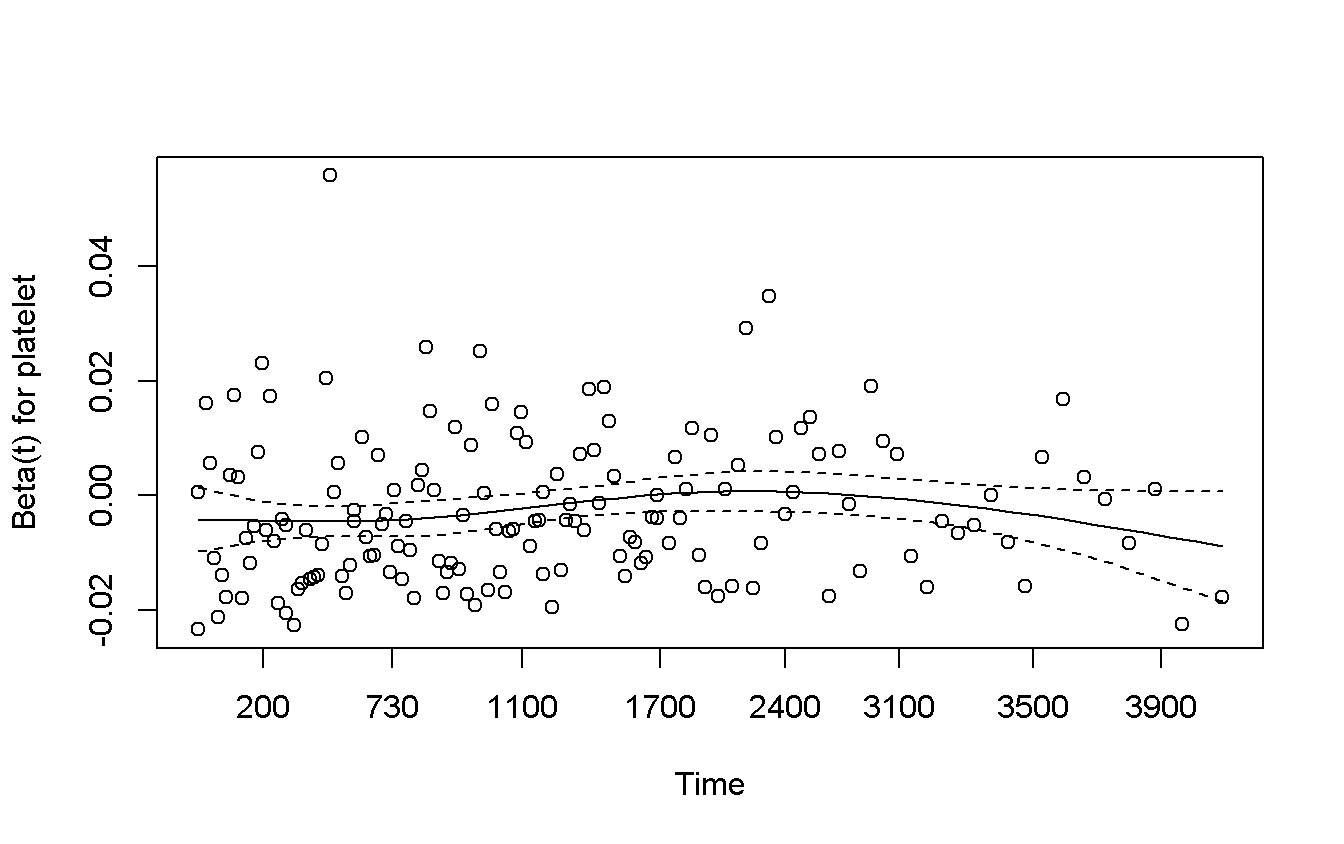
\includegraphics{SuDACDa-notes_files/figure-latex/unnamed-chunk-15-1.pdf}

\begin{Shaded}
\begin{Highlighting}[]
\KeywordTok{rcspline.plot}\NormalTok{(}
  \DataTypeTok{x       =} \NormalTok{pbc_df$platelet %>%}\StringTok{ }\NormalTok{as.numeric,}
  \DataTypeTok{y       =} \NormalTok{pbc_df$time,}
  \DataTypeTok{event   =} \NormalTok{pbc_df$status ==}\StringTok{ }\DecValTok{2}\NormalTok{,}
  \DataTypeTok{xlab    =} \StringTok{'Platelet'}\NormalTok{,}
  \DataTypeTok{statloc =} \StringTok{'ll'}
\NormalTok{)}
\end{Highlighting}
\end{Shaded}

\begin{verbatim}
##            x                                        
## -0.002304221 -0.034164621  0.159445107 -0.192976796 
## [1] -836.1424 -826.2939
\end{verbatim}

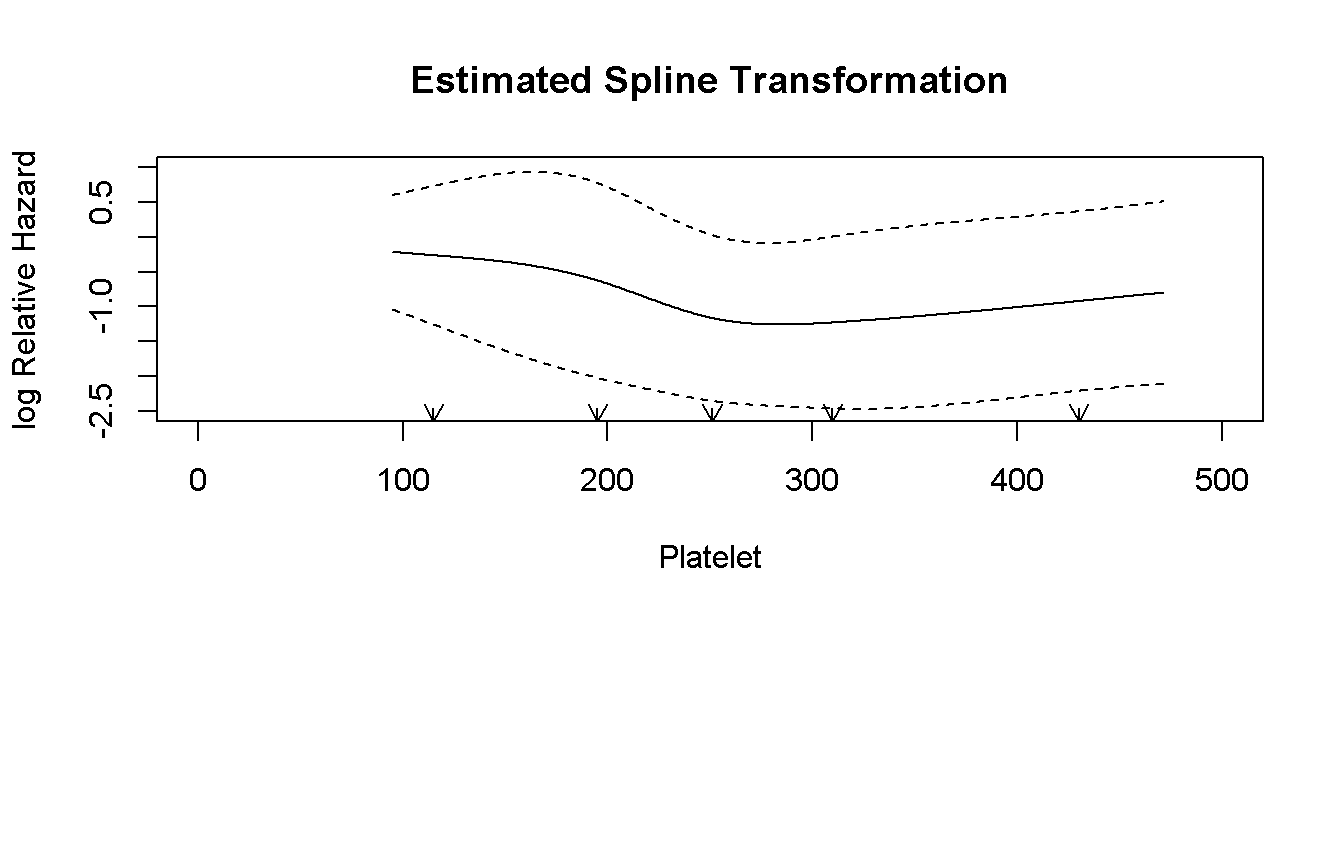
\includegraphics{SuDACDa-notes_files/figure-latex/unnamed-chunk-15-2.pdf}

\begin{verbatim}
## 
## cbind(xe, lower, upper)
## 
##               xe                        
##   [1,]  94.92629 -1.037889  0.6004264311
##   [2,]  95.55425 -1.044755  0.6043983883
##   [3,]  96.18221 -1.051620  0.6083703455
##   [4,]  96.81017 -1.058486  0.6123423027
##   [5,]  97.43813 -1.065352  0.6163142598
##   [6,]  98.06608 -1.072218  0.6202862170
##   [7,]  98.69404 -1.079084  0.6242581742
##   [8,]  99.32200 -1.085950  0.6282301314
##   [9,]  99.94996 -1.092816  0.6322020886
##  [10,] 100.57792 -1.099682  0.6361740458
##  [11,] 101.20588 -1.106547  0.6401460030
##  [12,] 101.83384 -1.113413  0.6441179602
##  [13,] 102.46180 -1.120279  0.6480899174
##  [14,] 103.08976 -1.127145  0.6520618746
##  [15,] 103.71772 -1.134011  0.6560338318
##  [16,] 104.34567 -1.140877  0.6600057890
##  [17,] 104.97363 -1.147743  0.6639777462
##  [18,] 105.60159 -1.154609  0.6679497034
##  [19,] 106.22955 -1.161474  0.6719216606
##  [20,] 106.85751 -1.168340  0.6758936178
##  [21,] 107.48547 -1.175206  0.6798655750
##  [22,] 108.11343 -1.182072  0.6838375322
##  [23,] 108.74139 -1.188938  0.6878094894
##  [24,] 109.36935 -1.195804  0.6917814466
##  [25,] 109.99731 -1.202670  0.6957534038
##  [26,] 110.62526 -1.209535  0.6997253610
##  [27,] 111.25322 -1.216401  0.7036973181
##  [28,] 111.88118 -1.223267  0.7076692753
##  [29,] 112.50914 -1.230133  0.7116412325
##  [30,] 113.13710 -1.236999  0.7156131897
##  [31,] 113.76506 -1.243865  0.7195851469
##  [32,] 114.39302 -1.250731  0.7235571041
##  [33,] 115.02098 -1.257597  0.7275290597
##  [34,] 115.64894 -1.264462  0.7315006305
##  [35,] 116.27689 -1.271328  0.7354705646
##  [36,] 116.90485 -1.278192  0.7394374895
##  [37,] 117.53281 -1.285056  0.7434000330
##  [38,] 118.16077 -1.291918  0.7473568226
##  [39,] 118.78873 -1.298778  0.7513064862
##  [40,] 119.41669 -1.305636  0.7552476513
##  [41,] 120.04465 -1.312491  0.7591789456
##  [42,] 120.67261 -1.319344  0.7630989971
##  [43,] 121.30057 -1.326193  0.7670064335
##  [44,] 121.92853 -1.333039  0.7708998828
##  [45,] 122.55648 -1.339881  0.7747779730
##  [46,] 123.18444 -1.346719  0.7786393322
##  [47,] 123.81240 -1.353552  0.7824825887
##  [48,] 124.44036 -1.360380  0.7863063711
##  [49,] 125.06832 -1.367203  0.7901093078
##  [50,] 125.69628 -1.374020  0.7938900277
##  [51,] 126.32424 -1.380831  0.7976471598
##  [52,] 126.95220 -1.387636  0.8013793336
##  [53,] 127.58016 -1.394434  0.8050851785
##  [54,] 128.20812 -1.401225  0.8087633245
##  [55,] 128.83607 -1.408009  0.8124124018
##  [56,] 129.46403 -1.414784  0.8160310411
##  [57,] 130.09199 -1.421552  0.8196178734
##  [58,] 130.71995 -1.428312  0.8231715301
##  [59,] 131.34791 -1.435062  0.8266906432
##  [60,] 131.97587 -1.441804  0.8301738453
##  [61,] 132.60383 -1.448535  0.8336197692
##  [62,] 133.23179 -1.455258  0.8370270486
##  [63,] 133.85975 -1.461970  0.8403943177
##  [64,] 134.48770 -1.468671  0.8437202114
##  [65,] 135.11566 -1.475362  0.8470033653
##  [66,] 135.74362 -1.482041  0.8502424157
##  [67,] 136.37158 -1.488709  0.8534359998
##  [68,] 136.99954 -1.495365  0.8565827555
##  [69,] 137.62750 -1.502009  0.8596813217
##  [70,] 138.25546 -1.508640  0.8627303382
##  [71,] 138.88342 -1.515258  0.8657284457
##  [72,] 139.51138 -1.521864  0.8686742860
##  [73,] 140.13934 -1.528455  0.8715665020
##  [74,] 140.76729 -1.535033  0.8744037377
##  [75,] 141.39525 -1.541597  0.8771846381
##  [76,] 142.02321 -1.548146  0.8799078498
##  [77,] 142.65117 -1.554680  0.8825720204
##  [78,] 143.27913 -1.561199  0.8851757989
##  [79,] 143.90709 -1.567702  0.8877178358
##  [80,] 144.53505 -1.574189  0.8901967829
##  [81,] 145.16301 -1.580661  0.8926112937
##  [82,] 145.79097 -1.587116  0.8949600232
##  [83,] 146.41893 -1.593554  0.8972416280
##  [84,] 147.04688 -1.599974  0.8994547664
##  [85,] 147.67484 -1.606378  0.9015980987
##  [86,] 148.30280 -1.612763  0.9036702867
##  [87,] 148.93076 -1.619131  0.9056699944
##  [88,] 149.55872 -1.625480  0.9075958876
##  [89,] 150.18668 -1.631810  0.9094466344
##  [90,] 150.81464 -1.638122  0.9112209047
##  [91,] 151.44260 -1.644414  0.9129173709
##  [92,] 152.07056 -1.650686  0.9145347075
##  [93,] 152.69851 -1.656939  0.9160715915
##  [94,] 153.32647 -1.663171  0.9175267023
##  [95,] 153.95443 -1.669383  0.9188987219
##  [96,] 154.58239 -1.675574  0.9201863348
##  [97,] 155.21035 -1.681744  0.9213882284
##  [98,] 155.83831 -1.687892  0.9225030926
##  [99,] 156.46627 -1.694019  0.9235296207
## [100,] 157.09423 -1.700124  0.9244665084
## [101,] 157.72219 -1.706206  0.9253124551
## [102,] 158.35015 -1.712266  0.9260661630
## [103,] 158.97810 -1.718303  0.9267263377
## [104,] 159.60606 -1.724318  0.9272916884
## [105,] 160.23402 -1.730308  0.9277609275
## [106,] 160.86198 -1.736276  0.9281327714
## [107,] 161.48994 -1.742219  0.9284059401
## [108,] 162.11790 -1.748139  0.9285791574
## [109,] 162.74586 -1.754034  0.9286511513
## [110,] 163.37382 -1.759904  0.9286206538
## [111,] 164.00178 -1.765750  0.9284864013
## [112,] 164.62974 -1.771570  0.9282471345
## [113,] 165.25769 -1.777366  0.9279015988
## [114,] 165.88565 -1.783135  0.9274485442
## [115,] 166.51361 -1.788879  0.9268867256
## [116,] 167.14157 -1.794597  0.9262149028
## [117,] 167.76953 -1.800289  0.9254318410
## [118,] 168.39749 -1.805955  0.9245363105
## [119,] 169.02545 -1.811594  0.9235270873
## [120,] 169.65341 -1.817206  0.9224029530
## [121,] 170.28137 -1.822791  0.9211626950
## [122,] 170.90932 -1.828349  0.9198051069
## [123,] 171.53728 -1.833879  0.9183289885
## [124,] 172.16524 -1.839383  0.9167331460
## [125,] 172.79320 -1.844858  0.9150163925
## [126,] 173.42116 -1.850306  0.9131775475
## [127,] 174.04912 -1.855725  0.9112154381
## [128,] 174.67708 -1.861117  0.9091288985
## [129,] 175.30504 -1.866480  0.9069167705
## [130,] 175.93300 -1.871815  0.9045779037
## [131,] 176.56096 -1.877121  0.9021111558
## [132,] 177.18891 -1.882399  0.8995153928
## [133,] 177.81687 -1.887648  0.8967894895
## [134,] 178.44483 -1.892869  0.8939323292
## [135,] 179.07279 -1.898060  0.8909428048
## [136,] 179.70075 -1.903222  0.8878198185
## [137,] 180.32871 -1.908356  0.8845622823
## [138,] 180.95667 -1.913460  0.8811691184
## [139,] 181.58463 -1.918535  0.8776392594
## [140,] 182.21259 -1.923581  0.8739716488
## [141,] 182.84055 -1.928598  0.8701652412
## [142,] 183.46850 -1.933585  0.8662190030
## [143,] 184.09646 -1.938544  0.8621319122
## [144,] 184.72442 -1.943473  0.8579029594
## [145,] 185.35238 -1.948373  0.8535311479
## [146,] 185.98034 -1.953244  0.8490154944
## [147,] 186.60830 -1.958086  0.8443550291
## [148,] 187.23626 -1.962898  0.8395487964
## [149,] 187.86422 -1.967682  0.8345958553
## [150,] 188.49218 -1.972437  0.8294952800
## [151,] 189.12013 -1.977163  0.8242461605
## [152,] 189.74809 -1.981861  0.8188476028
## [153,] 190.37605 -1.986530  0.8132987300
## [154,] 191.00401 -1.991171  0.8075986822
## [155,] 191.63197 -1.995784  0.8017466180
## [156,] 192.25993 -2.000369  0.7957417142
## [157,] 192.88789 -2.004927  0.7895831674
## [158,] 193.51585 -2.009457  0.7832701937
## [159,] 194.14381 -2.013959  0.7768020304
## [160,] 194.77177 -2.018435  0.7701779361
## [161,] 195.39972 -2.022884  0.7633974190
## [162,] 196.02768 -2.027308  0.7564629573
## [163,] 196.65564 -2.031706  0.7493790905
## [164,] 197.28360 -2.036080  0.7421503895
## [165,] 197.91156 -2.040430  0.7347814138
## [166,] 198.53952 -2.044758  0.7272767102
## [167,] 199.16748 -2.049063  0.7196408118
## [168,] 199.79544 -2.053348  0.7118782374
## [169,] 200.42340 -2.057612  0.7039934900
## [170,] 201.05136 -2.061857  0.6959910564
## [171,] 201.67931 -2.066083  0.6878754060
## [172,] 202.30727 -2.070290  0.6796509898
## [173,] 202.93523 -2.074480  0.6713222394
## [174,] 203.56319 -2.078653  0.6628935664
## [175,] 204.19115 -2.082810  0.6543693612
## [176,] 204.81911 -2.086951  0.6457539922
## [177,] 205.44707 -2.091077  0.6370518049
## [178,] 206.07503 -2.095189  0.6282671208
## [179,] 206.70299 -2.099287  0.6194042368
## [180,] 207.33094 -2.103371  0.6104674242
## [181,] 207.95890 -2.107443  0.6014609278
## [182,] 208.58686 -2.111502  0.5923889649
## [183,] 209.21482 -2.115549  0.5832557248
## [184,] 209.84278 -2.119585  0.5740653678
## [185,] 210.47074 -2.123609  0.5648220243
## [186,] 211.09870 -2.127622  0.5555297940
## [187,] 211.72666 -2.131626  0.5461927454
## [188,] 212.35462 -2.135618  0.5368149146
## [189,] 212.98258 -2.139601  0.5274003051
## [190,] 213.61053 -2.143574  0.5179528865
## [191,] 214.23849 -2.147538  0.5084765944
## [192,] 214.86645 -2.151492  0.4989753294
## [193,] 215.49441 -2.155437  0.4894529564
## [194,] 216.12237 -2.159372  0.4799133043
## [195,] 216.75033 -2.163299  0.4703601653
## [196,] 217.37829 -2.167216  0.4607972945
## [197,] 218.00625 -2.171124  0.4512284091
## [198,] 218.63421 -2.175023  0.4416571884
## [199,] 219.26217 -2.178912  0.4320872729
## [200,] 219.89012 -2.182792  0.4225222647
## [201,] 220.51808 -2.186662  0.4129657264
## [202,] 221.14604 -2.190522  0.4034211814
## [203,] 221.77400 -2.194372  0.3938921134
## [204,] 222.40196 -2.198211  0.3843819665
## [205,] 223.02992 -2.202040  0.3748941452
## [206,] 223.65788 -2.205857  0.3654320139
## [207,] 224.28584 -2.209663  0.3559988975
## [208,] 224.91380 -2.213456  0.3465980814
## [209,] 225.54175 -2.217237  0.3372328114
## [210,] 226.16971 -2.221005  0.3279062944
## [211,] 226.79767 -2.224759  0.3186216985
## [212,] 227.42563 -2.228498  0.3093821533
## [213,] 228.05359 -2.232223  0.3001907507
## [214,] 228.68155 -2.235932  0.2910505455
## [215,] 229.30951 -2.239624  0.2819645558
## [216,] 229.93747 -2.243299  0.2729357638
## [217,] 230.56543 -2.246956  0.2639671170
## [218,] 231.19339 -2.250594  0.2550615286
## [219,] 231.82134 -2.254213  0.2462218791
## [220,] 232.44930 -2.257811  0.2374510170
## [221,] 233.07726 -2.261387  0.2287517603
## [222,] 233.70522 -2.264940  0.2201268978
## [223,] 234.33318 -2.268471  0.2115791904
## [224,] 234.96114 -2.271976  0.2031113725
## [225,] 235.58910 -2.275456  0.1947261543
## [226,] 236.21706 -2.278910  0.1864262227
## [227,] 236.84502 -2.282335  0.1782142438
## [228,] 237.47298 -2.285732  0.1700928647
## [229,] 238.10093 -2.289099  0.1620647152
## [230,] 238.72889 -2.292435  0.1541324105
## [231,] 239.35685 -2.295739  0.1462985532
## [232,] 239.98481 -2.299009  0.1385657360
## [233,] 240.61277 -2.302245  0.1309365438
## [234,] 241.24073 -2.305445  0.1234135566
## [235,] 241.86869 -2.308608  0.1159993521
## [236,] 242.49665 -2.311733  0.1086965089
## [237,] 243.12461 -2.314818  0.1015076090
## [238,] 243.75256 -2.317864  0.0944352411
## [239,] 244.38052 -2.320868  0.0874820038
## [240,] 245.00848 -2.323829  0.0806505089
## [241,] 245.63644 -2.326746  0.0739433848
## [242,] 246.26440 -2.329619  0.0673632800
## [243,] 246.89236 -2.332445  0.0609128665
## [244,] 247.52032 -2.335225  0.0545948440
## [245,] 248.14828 -2.337956  0.0484119433
## [246,] 248.77624 -2.340639  0.0423669304
## [247,] 249.40420 -2.343271  0.0364626104
## [248,] 250.03215 -2.345853  0.0307018319
## [249,] 250.66011 -2.348383  0.0250874906
## [250,] 251.28807 -2.350860  0.0196224581
## [251,] 251.91603 -2.353285  0.0143075136
## [252,] 252.54399 -2.355657  0.0091411076
## [253,] 253.17195 -2.357977  0.0041216295
## [254,] 253.79991 -2.360246 -0.0007524692
## [255,] 254.42787 -2.362463 -0.0054826783
## [256,] 255.05583 -2.364631 -0.0100704316
## [257,] 255.68379 -2.366748 -0.0145171097
## [258,] 256.31174 -2.368816 -0.0188240432
## [259,] 256.93970 -2.370836 -0.0229925153
## [260,] 257.56766 -2.372809 -0.0270237650
## [261,] 258.19562 -2.374734 -0.0309189895
## [262,] 258.82358 -2.376614 -0.0346793478
## [263,] 259.45154 -2.378449 -0.0383059627
## [264,] 260.07950 -2.380240 -0.0417999242
## [265,] 260.70746 -2.381988 -0.0451622923
## [266,] 261.33542 -2.383693 -0.0483940993
## [267,] 261.96337 -2.385358 -0.0514963531
## [268,] 262.59133 -2.386983 -0.0544700397
## [269,] 263.21929 -2.388568 -0.0573161256
## [270,] 263.84725 -2.390116 -0.0600355611
## [271,] 264.47521 -2.391627 -0.0626292823
## [272,] 265.10317 -2.393103 -0.0650982139
## [273,] 265.73113 -2.394544 -0.0674432719
## [274,] 266.35909 -2.395951 -0.0696653660
## [275,] 266.98705 -2.397326 -0.0717654018
## [276,] 267.61501 -2.398670 -0.0737442834
## [277,] 268.24296 -2.399984 -0.0756029160
## [278,] 268.87092 -2.401269 -0.0773422078
## [279,] 269.49888 -2.402526 -0.0789630723
## [280,] 270.12684 -2.403756 -0.0804664307
## [281,] 270.75480 -2.404960 -0.0818532140
## [282,] 271.38276 -2.406140 -0.0831243649
## [283,] 272.01072 -2.407297 -0.0842808398
## [284,] 272.63868 -2.408431 -0.0853236111
## [285,] 273.26664 -2.409544 -0.0862536688
## [286,] 273.89460 -2.410636 -0.0870720222
## [287,] 274.52255 -2.411709 -0.0877797019
## [288,] 275.15051 -2.412763 -0.0883777617
## [289,] 275.77847 -2.413800 -0.0888672794
## [290,] 276.40643 -2.414821 -0.0892493593
## [291,] 277.03439 -2.415825 -0.0895251332
## [292,] 277.66235 -2.416815 -0.0896957615
## [293,] 278.29031 -2.417791 -0.0897624353
## [294,] 278.91827 -2.418754 -0.0897263770
## [295,] 279.54623 -2.419704 -0.0895888417
## [296,] 280.17418 -2.420643 -0.0893511182
## [297,] 280.80214 -2.421571 -0.0890145304
## [298,] 281.43010 -2.422488 -0.0885804376
## [299,] 282.05806 -2.423396 -0.0880502360
## [300,] 282.68602 -2.424295 -0.0874253590
## [301,] 283.31398 -2.425185 -0.0867072781
## [302,] 283.94194 -2.426068 -0.0858975039
## [303,] 284.56990 -2.426943 -0.0849975858
## [304,] 285.19786 -2.427810 -0.0840091135
## [305,] 285.82582 -2.428671 -0.0829337164
## [306,] 286.45377 -2.429526 -0.0817730649
## [307,] 287.08173 -2.430375 -0.0805288698
## [308,] 287.70969 -2.431218 -0.0792028833
## [309,] 288.33765 -2.432055 -0.0777968983
## [310,] 288.96561 -2.432887 -0.0763127490
## [311,] 289.59357 -2.433714 -0.0747523108
## [312,] 290.22153 -2.434536 -0.0731175001
## [313,] 290.84949 -2.435353 -0.0714102742
## [314,] 291.47745 -2.436165 -0.0696326308
## [315,] 292.10540 -2.436972 -0.0677866084
## [316,] 292.73336 -2.437774 -0.0658742851
## [317,] 293.36132 -2.438571 -0.0638977791
## [318,] 293.98928 -2.439363 -0.0618592474
## [319,] 294.61724 -2.440149 -0.0597608859
## [320,] 295.24520 -2.440930 -0.0576049283
## [321,] 295.87316 -2.441705 -0.0553936462
## [322,] 296.50112 -2.442473 -0.0531293478
## [323,] 297.12908 -2.443236 -0.0508143773
## [324,] 297.75704 -2.443991 -0.0484511144
## [325,] 298.38499 -2.444739 -0.0460419735
## [326,] 299.01295 -2.445480 -0.0435894024
## [327,] 299.64091 -2.446212 -0.0410958821
## [328,] 300.26887 -2.446936 -0.0385639252
## [329,] 300.89683 -2.447651 -0.0359960755
## [330,] 301.52479 -2.448356 -0.0333949068
## [331,] 302.15275 -2.449051 -0.0307630218
## [332,] 302.78071 -2.449735 -0.0281030514
## [333,] 303.40867 -2.450408 -0.0254176531
## [334,] 304.03663 -2.451068 -0.0227095106
## [335,] 304.66458 -2.451716 -0.0199813318
## [336,] 305.29254 -2.452350 -0.0172358486
## [337,] 305.92050 -2.452970 -0.0144758153
## [338,] 306.54846 -2.453575 -0.0117040071
## [339,] 307.17642 -2.454165 -0.0089232196
## [340,] 307.80438 -2.454737 -0.0061362672
## [341,] 308.43234 -2.455293 -0.0033459818
## [342,] 309.06030 -2.455830 -0.0005552118
## [343,] 309.68826 -2.456349  0.0022331794
## [344,] 310.31621 -2.456847  0.0050166817
## [345,] 310.94417 -2.457325  0.0077943373
## [346,] 311.57213 -2.457783  0.0105656164
## [347,] 312.20009 -2.458219  0.0133300085
## [348,] 312.82805 -2.458634  0.0160870225
## [349,] 313.45601 -2.459026  0.0188361859
## [350,] 314.08397 -2.459396  0.0215770445
## [351,] 314.71193 -2.459744  0.0243091620
## [352,] 315.33989 -2.460068  0.0270321197
## [353,] 315.96785 -2.460369  0.0297455161
## [354,] 316.59580 -2.460646  0.0324489666
## [355,] 317.22376 -2.460899  0.0351421029
## [356,] 317.85172 -2.461128  0.0378245729
## [357,] 318.47968 -2.461332  0.0404960404
## [358,] 319.10764 -2.461511  0.0431561843
## [359,] 319.73560 -2.461666  0.0458046989
## [360,] 320.36356 -2.461795  0.0484412931
## [361,] 320.99152 -2.461899  0.0510656904
## [362,] 321.61948 -2.461977  0.0536776281
## [363,] 322.24744 -2.462029  0.0562768576
## [364,] 322.87539 -2.462055  0.0588631438
## [365,] 323.50335 -2.462055  0.0614362648
## [366,] 324.13131 -2.462029  0.0639960113
## [367,] 324.75927 -2.461976  0.0665421872
## [368,] 325.38723 -2.461897  0.0690746082
## [369,] 326.01519 -2.461792  0.0715931024
## [370,] 326.64315 -2.461659  0.0740975096
## [371,] 327.27111 -2.461500  0.0765876813
## [372,] 327.89907 -2.461314  0.0790634799
## [373,] 328.52702 -2.461102  0.0815247792
## [374,] 329.15498 -2.460862  0.0839714636
## [375,] 329.78294 -2.460596  0.0864034280
## [376,] 330.41090 -2.460302  0.0888205778
## [377,] 331.03886 -2.459982  0.0912228281
## [378,] 331.66682 -2.459634  0.0936101043
## [379,] 332.29478 -2.459260  0.0959823409
## [380,] 332.92274 -2.458859  0.0983394820
## [381,] 333.55070 -2.458431  0.1006814811
## [382,] 334.17866 -2.457976  0.1030083003
## [383,] 334.80661 -2.457494  0.1053199105
## [384,] 335.43457 -2.456986  0.1076162914
## [385,] 336.06253 -2.456451  0.1098974307
## [386,] 336.69049 -2.455889  0.1121633245
## [387,] 337.31845 -2.455301  0.1144139768
## [388,] 337.94641 -2.454686  0.1166493992
## [389,] 338.57437 -2.454045  0.1188696112
## [390,] 339.20233 -2.453378  0.1210746393
## [391,] 339.83029 -2.452684  0.1232645177
## [392,] 340.45825 -2.451965  0.1254392873
## [393,] 341.08620 -2.451219  0.1275989960
## [394,] 341.71416 -2.450448  0.1297436984
## [395,] 342.34212 -2.449652  0.1318734557
## [396,] 342.97008 -2.448829  0.1339883356
## [397,] 343.59804 -2.447982  0.1360884117
## [398,] 344.22600 -2.447109  0.1381737640
## [399,] 344.85396 -2.446211  0.1402444785
## [400,] 345.48192 -2.445289  0.1423006466
## [401,] 346.10988 -2.444341  0.1443423656
## [402,] 346.73783 -2.443370  0.1463697384
## [403,] 347.36579 -2.442374  0.1483828731
## [404,] 347.99375 -2.441353  0.1503818830
## [405,] 348.62171 -2.440309  0.1523668865
## [406,] 349.24967 -2.439241  0.1543380071
## [407,] 349.87763 -2.438150  0.1562953730
## [408,] 350.50559 -2.437035  0.1582391170
## [409,] 351.13355 -2.435898  0.1601693767
## [410,] 351.76151 -2.434737  0.1620862940
## [411,] 352.38947 -2.433554  0.1639900150
## [412,] 353.01742 -2.432348  0.1658806904
## [413,] 353.64538 -2.431120  0.1677584745
## [414,] 354.27334 -2.429870  0.1696235260
## [415,] 354.90130 -2.428598  0.1714760071
## [416,] 355.52926 -2.427305  0.1733160839
## [417,] 356.15722 -2.425991  0.1751439262
## [418,] 356.78518 -2.424655  0.1769597071
## [419,] 357.41314 -2.423299  0.1787636035
## [420,] 358.04110 -2.421923  0.1805557951
## [421,] 358.66906 -2.420526  0.1823364652
## [422,] 359.29701 -2.419109  0.1841058001
## [423,] 359.92497 -2.417673  0.1858639889
## [424,] 360.55293 -2.416217  0.1876112239
## [425,] 361.18089 -2.414742  0.1893476999
## [426,] 361.80885 -2.413248  0.1910736147
## [427,] 362.43681 -2.411735  0.1927891684
## [428,] 363.06477 -2.410204  0.1944945638
## [429,] 363.69273 -2.408655  0.1961900061
## [430,] 364.32069 -2.407088  0.1978757027
## [431,] 364.94864 -2.405504  0.1995518634
## [432,] 365.57660 -2.403903  0.2012187000
## [433,] 366.20456 -2.402284  0.2028764263
## [434,] 366.83252 -2.400650  0.2045252583
## [435,] 367.46048 -2.398998  0.2061654135
## [436,] 368.08844 -2.397331  0.2077971115
## [437,] 368.71640 -2.395648  0.2094205734
## [438,] 369.34436 -2.393950  0.2110360221
## [439,] 369.97232 -2.392236  0.2126436817
## [440,] 370.60028 -2.390508  0.2142437781
## [441,] 371.22823 -2.388765  0.2158365383
## [442,] 371.85619 -2.387008  0.2174221907
## [443,] 372.48415 -2.385237  0.2190009648
## [444,] 373.11211 -2.383452  0.2205730912
## [445,] 373.74007 -2.381654  0.2221388017
## [446,] 374.36803 -2.379843  0.2236983288
## [447,] 374.99599 -2.378020  0.2252519061
## [448,] 375.62395 -2.376184  0.2267997677
## [449,] 376.25191 -2.374336  0.2283421487
## [450,] 376.87987 -2.372476  0.2298792847
## [451,] 377.50782 -2.370605  0.2314114118
## [452,] 378.13578 -2.368722  0.2329387666
## [453,] 378.76374 -2.366829  0.2344615863
## [454,] 379.39170 -2.364926  0.2359801082
## [455,] 380.01966 -2.363012  0.2374945699
## [456,] 380.64762 -2.361088  0.2390052091
## [457,] 381.27558 -2.359155  0.2405122638
## [458,] 381.90354 -2.357212  0.2420159719
## [459,] 382.53150 -2.355261  0.2435165712
## [460,] 383.15945 -2.353301  0.2450142996
## [461,] 383.78741 -2.351333  0.2465093944
## [462,] 384.41537 -2.349356  0.2480020932
## [463,] 385.04333 -2.347372  0.2494926327
## [464,] 385.67129 -2.345381  0.2509812497
## [465,] 386.29925 -2.343383  0.2524681801
## [466,] 386.92721 -2.341377  0.2539536594
## [467,] 387.55517 -2.339366  0.2554379227
## [468,] 388.18313 -2.337348  0.2569212040
## [469,] 388.81109 -2.335325  0.2584037370
## [470,] 389.43904 -2.333296  0.2598857542
## [471,] 390.06700 -2.331262  0.2613674875
## [472,] 390.69496 -2.329223  0.2628491675
## [473,] 391.32292 -2.327179  0.2643310241
## [474,] 391.95088 -2.325131  0.2658132860
## [475,] 392.57884 -2.323079  0.2672961806
## [476,] 393.20680 -2.321024  0.2687799344
## [477,] 393.83476 -2.318965  0.2702647722
## [478,] 394.46272 -2.316903  0.2717509177
## [479,] 395.09068 -2.314838  0.2732385932
## [480,] 395.71863 -2.312771  0.2747280194
## [481,] 396.34659 -2.310701  0.2762194156
## [482,] 396.97455 -2.308630  0.2777129992
## [483,] 397.60251 -2.306557  0.2792089862
## [484,] 398.23047 -2.304483  0.2807075908
## [485,] 398.85843 -2.302408  0.2822090254
## [486,] 399.48639 -2.300332  0.2837135005
## [487,] 400.11435 -2.298256  0.2852212248
## [488,] 400.74231 -2.296179  0.2867324048
## [489,] 401.37026 -2.294103  0.2882472451
## [490,] 401.99822 -2.292027  0.2897659483
## [491,] 402.62618 -2.289952  0.2912887148
## [492,] 403.25414 -2.287877  0.2928157426
## [493,] 403.88210 -2.285804  0.2943472277
## [494,] 404.51006 -2.283732  0.2958833636
## [495,] 405.13802 -2.281663  0.2974243415
## [496,] 405.76598 -2.279595  0.2989703502
## [497,] 406.39394 -2.277529  0.3005215759
## [498,] 407.02190 -2.275466  0.3020782025
## [499,] 407.64985 -2.273406  0.3036404110
## [500,] 408.27781 -2.271349  0.3052083799
## [501,] 408.90577 -2.269295  0.3067822851
## [502,] 409.53373 -2.267244  0.3083622997
## [503,] 410.16169 -2.265198  0.3099485940
## [504,] 410.78965 -2.263156  0.3115413354
## [505,] 411.41761 -2.261117  0.3131406885
## [506,] 412.04557 -2.259084  0.3147468150
## [507,] 412.67353 -2.257055  0.3163598736
## [508,] 413.30149 -2.255031  0.3179800199
## [509,] 413.92944 -2.253012  0.3196074065
## [510,] 414.55740 -2.250999  0.3212421829
## [511,] 415.18536 -2.248991  0.3228844956
## [512,] 415.81332 -2.246990  0.3245344876
## [513,] 416.44128 -2.244994  0.3261922990
## [514,] 417.06924 -2.243005  0.3278580664
## [515,] 417.69720 -2.241022  0.3295319233
## [516,] 418.32516 -2.239046  0.3312139997
## [517,] 418.95312 -2.237077  0.3329044223
## [518,] 419.58107 -2.235115  0.3346033144
## [519,] 420.20903 -2.233161  0.3363107960
## [520,] 420.83699 -2.231214  0.3380269834
## [521,] 421.46495 -2.229274  0.3397519896
## [522,] 422.09291 -2.227343  0.3414859240
## [523,] 422.72087 -2.225419  0.3432288924
## [524,] 423.34883 -2.223504  0.3449809972
## [525,] 423.97679 -2.221597  0.3467423370
## [526,] 424.60475 -2.219699  0.3485130069
## [527,] 425.23271 -2.217810  0.3502930984
## [528,] 425.86066 -2.215930  0.3520826993
## [529,] 426.48862 -2.214058  0.3538818936
## [530,] 427.11658 -2.212196  0.3556907617
## [531,] 427.74454 -2.210344  0.3575093804
## [532,] 428.37250 -2.208500  0.3593378226
## [533,] 429.00046 -2.206667  0.3611761575
## [534,] 429.62842 -2.204843  0.3630244507
## [535,] 430.25638 -2.203030  0.3648827631
## [536,] 430.88434 -2.201226  0.3667511282
## [537,] 431.51230 -2.199433  0.3686295472
## [538,] 432.14025 -2.197649  0.3705180192
## [539,] 432.76821 -2.195876  0.3724165430
## [540,] 433.39617 -2.194113  0.3743251169
## [541,] 434.02413 -2.192359  0.3762437394
## [542,] 434.65209 -2.190616  0.3781724086
## [543,] 435.28005 -2.188883  0.3801111221
## [544,] 435.90801 -2.187160  0.3820598777
## [545,] 436.53597 -2.185447  0.3840186727
## [546,] 437.16393 -2.183744  0.3859875041
## [547,] 437.79188 -2.182050  0.3879663690
## [548,] 438.41984 -2.180367  0.3899552639
## [549,] 439.04780 -2.178694  0.3919541852
## [550,] 439.67576 -2.177031  0.3939631292
## [551,] 440.30372 -2.175379  0.3959820918
## [552,] 440.93168 -2.173736  0.3980110686
## [553,] 441.55964 -2.172103  0.4000500554
## [554,] 442.18760 -2.170480  0.4020990471
## [555,] 442.81556 -2.168867  0.4041580390
## [556,] 443.44352 -2.167264  0.4062270258
## [557,] 444.07147 -2.165671  0.4083060021
## [558,] 444.69943 -2.164088  0.4103949621
## [559,] 445.32739 -2.162515  0.4124939001
## [560,] 445.95535 -2.160952  0.4146028099
## [561,] 446.58331 -2.159399  0.4167216852
## [562,] 447.21127 -2.157856  0.4188505194
## [563,] 447.83923 -2.156323  0.4209893058
## [564,] 448.46719 -2.154800  0.4231380372
## [565,] 449.09515 -2.153286  0.4252967065
## [566,] 449.72311 -2.151783  0.4274653062
## [567,] 450.35106 -2.150290  0.4296438287
## [568,] 450.97902 -2.148806  0.4318322659
## [569,] 451.60698 -2.147332  0.4340306099
## [570,] 452.23494 -2.145869  0.4362388522
## [571,] 452.86290 -2.144415  0.4384569843
## [572,] 453.49086 -2.142971  0.4406849975
## [573,] 454.11882 -2.141537  0.4429228826
## [574,] 454.74678 -2.140113  0.4451706306
## [575,] 455.37474 -2.138699  0.4474282320
## [576,] 456.00269 -2.137294  0.4496956772
## [577,] 456.63065 -2.135899  0.4519729562
## [578,] 457.25861 -2.134515  0.4542600591
## [579,] 457.88657 -2.133140  0.4565569756
## [580,] 458.51453 -2.131774  0.4588636952
## [581,] 459.14249 -2.130419  0.4611802073
## [582,] 459.77045 -2.129073  0.4635065008
## [583,] 460.39841 -2.127738  0.4658425648
## [584,] 461.02637 -2.126411  0.4681883880
## [585,] 461.65433 -2.125095  0.4705439588
## [586,] 462.28228 -2.123789  0.4729092655
## [587,] 462.91024 -2.122492  0.4752842962
## [588,] 463.53820 -2.121204  0.4776690389
## [589,] 464.16616 -2.119927  0.4800634812
## [590,] 464.79412 -2.118659  0.4824676107
## [591,] 465.42208 -2.117401  0.4848814145
## [592,] 466.05004 -2.116153  0.4873048800
## [593,] 466.67800 -2.114914  0.4897379939
## [594,] 467.30596 -2.113685  0.4921807431
## [595,] 467.93392 -2.112465  0.4946331140
## [596,] 468.56187 -2.111255  0.4970950930
## [597,] 469.18983 -2.110055  0.4995666663
## [598,] 469.81779 -2.108864  0.5020478199
## [599,] 470.44575 -2.107683  0.5045385396
## [600,] 471.07371 -2.106511  0.5070388110
\end{verbatim}

The log-linear plot has a U-shape so, standard transformation are not
good. We can try to perform a categorization. Two strategy: 1. look at
the log-linear plot and try to find a good cut-points, but we have to
explain how we have defined them (and ``use the p-value'' is not a good
strategy) 2. Use standard non related cutoff, such as median or
quartiles

\begin{Shaded}
\begin{Highlighting}[]
\NormalTok{cox_cut_platelet <-}\StringTok{ }\KeywordTok{coxph}\NormalTok{(}
  \KeywordTok{Surv}\NormalTok{(time, status ==}\StringTok{ }\DecValTok{2}\NormalTok{) ~}\StringTok{ }\KeywordTok{cut}\NormalTok{(platelet, }\KeywordTok{c}\NormalTok{(}\DecValTok{0}\NormalTok{, }\DecValTok{150}\NormalTok{, }\DecValTok{400}\NormalTok{, }\DecValTok{1000}\NormalTok{)),}
  \DataTypeTok{data =} \NormalTok{pbc_df}
\NormalTok{)}

\KeywordTok{cox.zph}\NormalTok{(cox_cut_platelet)}
\end{Highlighting}
\end{Shaded}

\begin{verbatim}
##                                                    rho   chisq     p
## cut(platelet, c(0, 150, 400, 1000))(150,400]   0.06413 0.62938 0.428
## cut(platelet, c(0, 150, 400, 1000))(400,1e+03] 0.00345 0.00181 0.966
## GLOBAL                                              NA 0.74607 0.689
\end{verbatim}

\begin{Shaded}
\begin{Highlighting}[]
\KeywordTok{cox.zph}\NormalTok{(cox_cut_platelet) %>%}
\StringTok{  }\KeywordTok{plot}\NormalTok{(}\DataTypeTok{col =} \StringTok{'blue'}\NormalTok{)}
\end{Highlighting}
\end{Shaded}

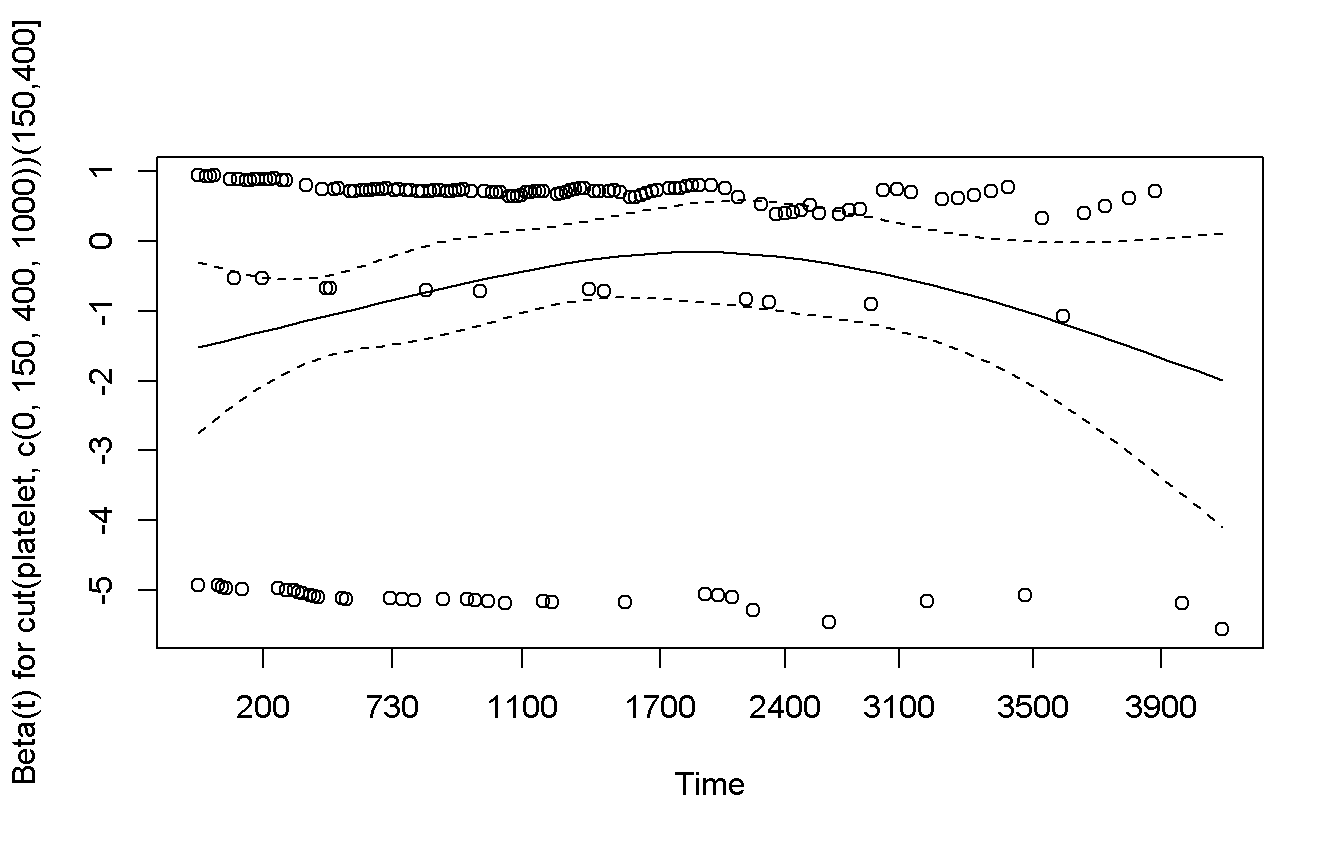
\includegraphics{SuDACDa-notes_files/figure-latex/unnamed-chunk-16-1.pdf}
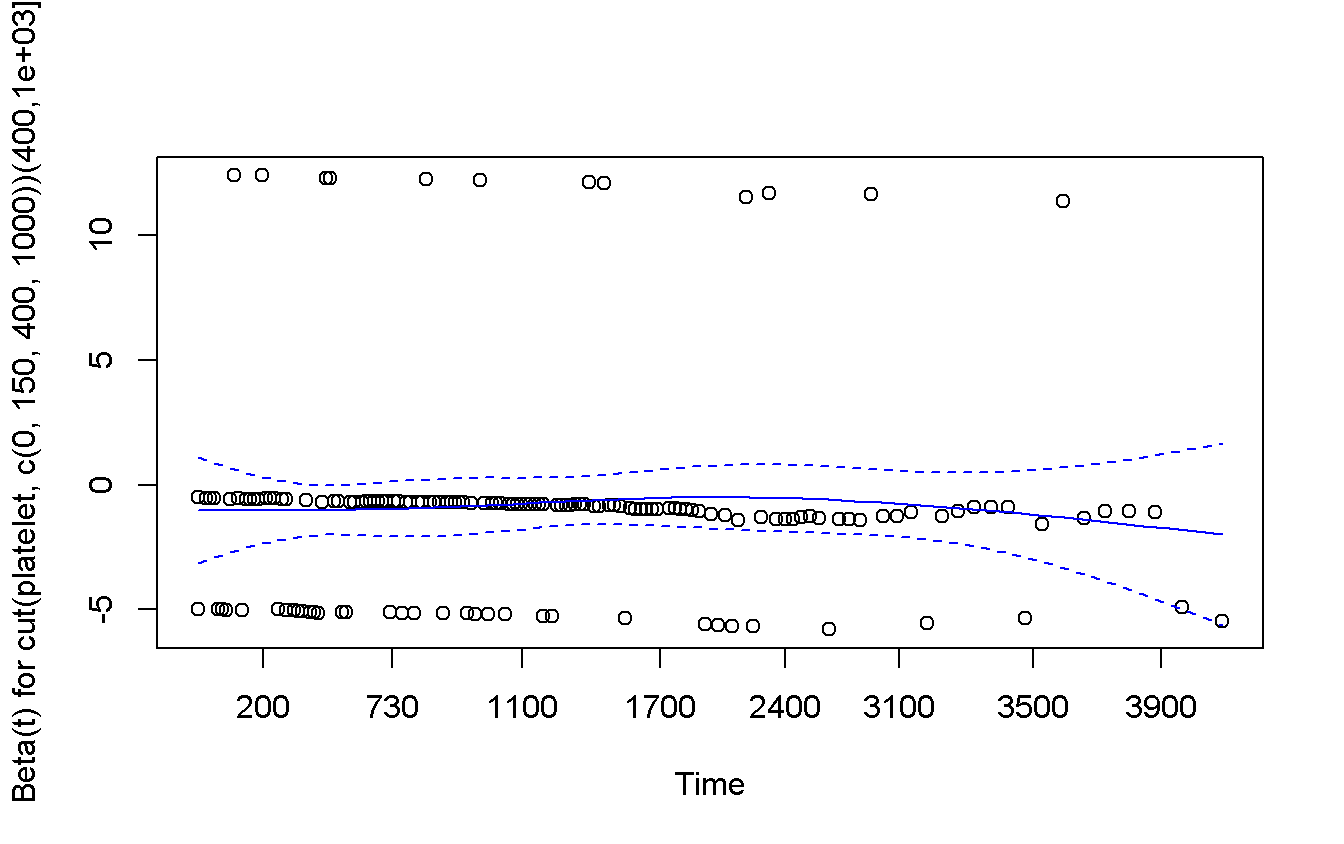
\includegraphics{SuDACDa-notes_files/figure-latex/unnamed-chunk-16-2.pdf}

\begin{Shaded}
\begin{Highlighting}[]
\KeywordTok{summary}\NormalTok{(cox_cut_platelet)}
\end{Highlighting}
\end{Shaded}

\begin{verbatim}
## Call:
## coxph(formula = Surv(time, status == 2) ~ cut(platelet, c(0, 
##     150, 400, 1000)), data = pbc_df)
## 
##   n= 407, number of events= 155 
##    (11 observations deleted due to missingness)
## 
##                                                   coef exp(coef) se(coef)
## cut(platelet, c(0, 150, 400, 1000))(150,400]   -0.7164    0.4885   0.1948
## cut(platelet, c(0, 150, 400, 1000))(400,1e+03] -0.8445    0.4298   0.3352
##                                                     z Pr(>|z|)    
## cut(platelet, c(0, 150, 400, 1000))(150,400]   -3.678 0.000235 ***
## cut(platelet, c(0, 150, 400, 1000))(400,1e+03] -2.519 0.011755 *  
## ---
## Signif. codes:  0 '***' 0.001 '**' 0.01 '*' 0.05 '.' 0.1 ' ' 1
## 
##                                                exp(coef) exp(-coef)
## cut(platelet, c(0, 150, 400, 1000))(150,400]      0.4885      2.047
## cut(platelet, c(0, 150, 400, 1000))(400,1e+03]    0.4298      2.327
##                                                lower .95 upper .95
## cut(platelet, c(0, 150, 400, 1000))(150,400]      0.3335    0.7156
## cut(platelet, c(0, 150, 400, 1000))(400,1e+03]    0.2228    0.8290
## 
## Concordance= 0.561  (se = 0.018 )
## Rsquare= 0.031   (max possible= 0.984 )
## Likelihood ratio test= 12.68  on 2 df,   p=0.001766
## Wald test            = 14.53  on 2 df,   p=0.0006987
## Score (logrank) test = 15.19  on 2 df,   p=0.0005032
\end{verbatim}

But here the reference level, i.e.~the contrast, is the lower level but
the interested is what happen if we lie above or over the standard
values, so we have to relevel the category to make the medium level as
the reference one, i.e.~the first.

\begin{Shaded}
\begin{Highlighting}[]
\NormalTok{pbc_df <-}\StringTok{ }\NormalTok{pbc_df %>%}\StringTok{ }
\StringTok{  }\KeywordTok{mutate}\NormalTok{(}
    \DataTypeTok{platelet_ref =} \KeywordTok{cut}\NormalTok{(pbc_df$platelet, }\KeywordTok{c}\NormalTok{(}\DecValTok{0}\NormalTok{, }\DecValTok{150}\NormalTok{, }\DecValTok{400}\NormalTok{, }\DecValTok{1000}\NormalTok{)) %>%}
\StringTok{                      }\KeywordTok{relevel}\NormalTok{(}\DataTypeTok{ref =} \StringTok{"(150,400]"}\NormalTok{)}
\NormalTok{)}

\NormalTok{cox_relev_platelet <-}\StringTok{ }\KeywordTok{coxph}\NormalTok{(}\KeywordTok{Surv}\NormalTok{(time, status ==}\StringTok{ }\DecValTok{2}\NormalTok{) ~}\StringTok{ }\NormalTok{platelet_ref,}
  \DataTypeTok{data =} \NormalTok{pbc_df}
\NormalTok{)}

\KeywordTok{summary}\NormalTok{(cox_relev_platelet)}
\end{Highlighting}
\end{Shaded}

\begin{verbatim}
## Call:
## coxph(formula = Surv(time, status == 2) ~ platelet_ref, data = pbc_df)
## 
##   n= 407, number of events= 155 
##    (11 observations deleted due to missingness)
## 
##                            coef exp(coef) se(coef)      z Pr(>|z|)    
## platelet_ref(0,150]      0.7164    2.0471   0.1948  3.678 0.000235 ***
## platelet_ref(400,1e+03] -0.1281    0.8798   0.3046 -0.420 0.674235    
## ---
## Signif. codes:  0 '***' 0.001 '**' 0.01 '*' 0.05 '.' 0.1 ' ' 1
## 
##                         exp(coef) exp(-coef) lower .95 upper .95
## platelet_ref(0,150]        2.0471     0.4885    1.3975     2.999
## platelet_ref(400,1e+03]    0.8798     1.1366    0.4843     1.598
## 
## Concordance= 0.561  (se = 0.018 )
## Rsquare= 0.031   (max possible= 0.984 )
## Likelihood ratio test= 12.68  on 2 df,   p=0.001766
## Wald test            = 14.53  on 2 df,   p=0.0006987
## Score (logrank) test = 15.19  on 2 df,   p=0.0005032
\end{verbatim}

\section{Investigation on adjusted variables and
interactions}\label{adjusted2}

Clinician: what is the effect of treatment (\texttt{trt}) on death?

\begin{Shaded}
\begin{Highlighting}[]
\KeywordTok{cph}\NormalTok{(}\KeywordTok{Surv}\NormalTok{(time, status ==}\StringTok{ }\DecValTok{2}\NormalTok{) ~}\StringTok{ }\NormalTok{trt,}
  \DataTypeTok{data =} \NormalTok{pbc_df}
\NormalTok{) %>%}\StringTok{ }
\StringTok{  }\NormalTok{summary}
\end{Highlighting}
\end{Shaded}

\begin{verbatim}
##              Effects              Response : Surv(time, status == 2) 
## 
##  Factor        Low High Diff. Effect    S.E.    Lower 0.95 Upper 0.95
##  trt           1   2    1     -0.057189 0.17916 -0.40835   0.29397   
##   Hazard Ratio 1   2    1      0.944420      NA  0.66475   1.34170
\end{verbatim}

No significant effect for treatment.

Clinician: an adjusted with edema?

\begin{Shaded}
\begin{Highlighting}[]
\KeywordTok{cph}\NormalTok{(}\KeywordTok{Surv}\NormalTok{(time, status ==}\StringTok{ }\DecValTok{2}\NormalTok{) ~}\StringTok{ }\NormalTok{trt +}\StringTok{ }\NormalTok{edema,}
  \DataTypeTok{data =} \NormalTok{pbc_df}
\NormalTok{) %>%}\StringTok{ }
\StringTok{  }\NormalTok{summary}
\end{Highlighting}
\end{Shaded}

\begin{verbatim}
##              Effects              Response : Surv(time, status == 2) 
## 
##  Factor        Low High Diff. Effect    S.E.    Lower 0.95 Upper 0.95
##  trt           1   2    1     -0.065946 0.17953 -0.41781    0.28592  
##   Hazard Ratio 1   2    1      0.936180      NA  0.65849    1.33100  
##  edema         0   1    1      2.280700 0.25761  1.77580    2.78560  
##   Hazard Ratio 0   1    1      9.783600      NA  5.90510   16.21000
\end{verbatim}

No effect for treatment nor edema

Clinicians: and what about their interaction?\footnote{The answer here
  should be ``if there are no marginal significant effect is has no
  sense to look at the interaction terms!''.}

\begin{Shaded}
\begin{Highlighting}[]
\KeywordTok{cph}\NormalTok{(}\KeywordTok{Surv}\NormalTok{(time, status ==}\StringTok{ }\DecValTok{2}\NormalTok{) ~}\StringTok{ }\NormalTok{trt *}\StringTok{ }\NormalTok{edema,}
  \DataTypeTok{data =} \NormalTok{pbc_df}
\NormalTok{) %>%}\StringTok{ }
\StringTok{  }\NormalTok{summary}
\end{Highlighting}
\end{Shaded}

\begin{verbatim}
##              Effects              Response : Surv(time, status == 2) 
## 
##  Factor        Low High Diff. Effect   S.E.    Lower 0.95 Upper 0.95
##  trt           1   2    1     -0.24014 0.22959 -0.69012    0.20984  
##   Hazard Ratio 1   2    1      0.78652      NA  0.50151    1.23350  
##  edema         0   1    1      2.62340 0.37161  1.89500    3.35170  
##   Hazard Ratio 0   1    1     13.78200      NA  6.65280   28.55200  
## 
## Adjusted to: trt=1 edema=0.5
\end{verbatim}

No effect.

Clinicians: and what about adjusted with stage?

\begin{Shaded}
\begin{Highlighting}[]
\NormalTok{adj_pbc <-}\StringTok{ }\NormalTok{pbc_df %>%}\StringTok{ }
\StringTok{  }\KeywordTok{mutate}\NormalTok{(}\DataTypeTok{stage_fct =} \KeywordTok{factor}\NormalTok{(stage))}

\NormalTok{dd <-}\StringTok{ }\KeywordTok{datadist}\NormalTok{(adj_pbc)}

\KeywordTok{cph}\NormalTok{(}\KeywordTok{Surv}\NormalTok{(time, status ==}\StringTok{ }\DecValTok{2}\NormalTok{) ~}\StringTok{ }\NormalTok{trt +}\StringTok{ }\NormalTok{stage_fct,}
  \DataTypeTok{data =} \NormalTok{adj_pbc}
\NormalTok{) %>%}\StringTok{ }
\StringTok{  }\NormalTok{summary}
\end{Highlighting}
\end{Shaded}

\begin{verbatim}
##              Effects              Response : Surv(time, status == 2) 
## 
##  Factor          Low High Diff. Effect   S.E.    Lower 0.95 Upper 0.95
##  trt             1   2     1    -0.14713 0.17989 -0.49971    0.20545  
##   Hazard Ratio   1   2     1     0.86318      NA  0.60671    1.22810  
##  stage_fct - 1:3 3   1    NA    -2.17290 1.01080 -4.15410   -0.19176  
##   Hazard Ratio   3   1    NA     0.11384      NA  0.01570    0.82550  
##  stage_fct - 2:3 3   2    NA    -0.54826 0.29344 -1.12340    0.02687  
##   Hazard Ratio   3   2    NA     0.57795      NA  0.32517    1.02720  
##  stage_fct - 4:3 3   4    NA     0.91613 0.19771  0.52862    1.30360  
##   Hazard Ratio   3   4    NA     2.49960      NA  1.69660    3.68270
\end{verbatim}

Treatment still with no significant effect. \texttt{stage} has some
effects, i.e.~from the 3 to 1 or to 4,

Clinicians: oh, so let's look at the interactions!

\begin{Shaded}
\begin{Highlighting}[]
\NormalTok{rms_trt_stage <-}\StringTok{ }\KeywordTok{cph}\NormalTok{(}\KeywordTok{Surv}\NormalTok{(time, status ==}\StringTok{ }\DecValTok{2}\NormalTok{) ~}\StringTok{ }\NormalTok{trt *}\StringTok{ }\NormalTok{stage,}
  \DataTypeTok{data =} \NormalTok{adj_pbc}
\NormalTok{)}

\KeywordTok{summary}\NormalTok{(rms_trt_stage)}
\end{Highlighting}
\end{Shaded}

\begin{verbatim}
##              Effects              Response : Surv(time, status == 2) 
## 
##  Factor        Low High Diff. Effect   S.E.    Lower 0.95 Upper 0.95
##  trt           1   2    1     -0.15717 0.20284 -0.55473   0.24039   
##   Hazard Ratio 1   2    1      0.85456      NA  0.57423   1.27170   
##  stage         2   4    2      1.61630 0.33135  0.96682   2.26570   
##   Hazard Ratio 2   4    2      5.03420      NA  2.62960   9.63790   
## 
## Adjusted to: trt=1 stage=3
\end{verbatim}

\begin{Shaded}
\begin{Highlighting}[]
\KeywordTok{Predict}\NormalTok{(rms_trt_stage) %>%}
\StringTok{  }\KeywordTok{ggplot}\NormalTok{(}\DataTypeTok{anova =} \KeywordTok{anova}\NormalTok{(rms_trt_stage), }\DataTypeTok{pval =} \OtherTok{TRUE}\NormalTok{)}
\end{Highlighting}
\end{Shaded}

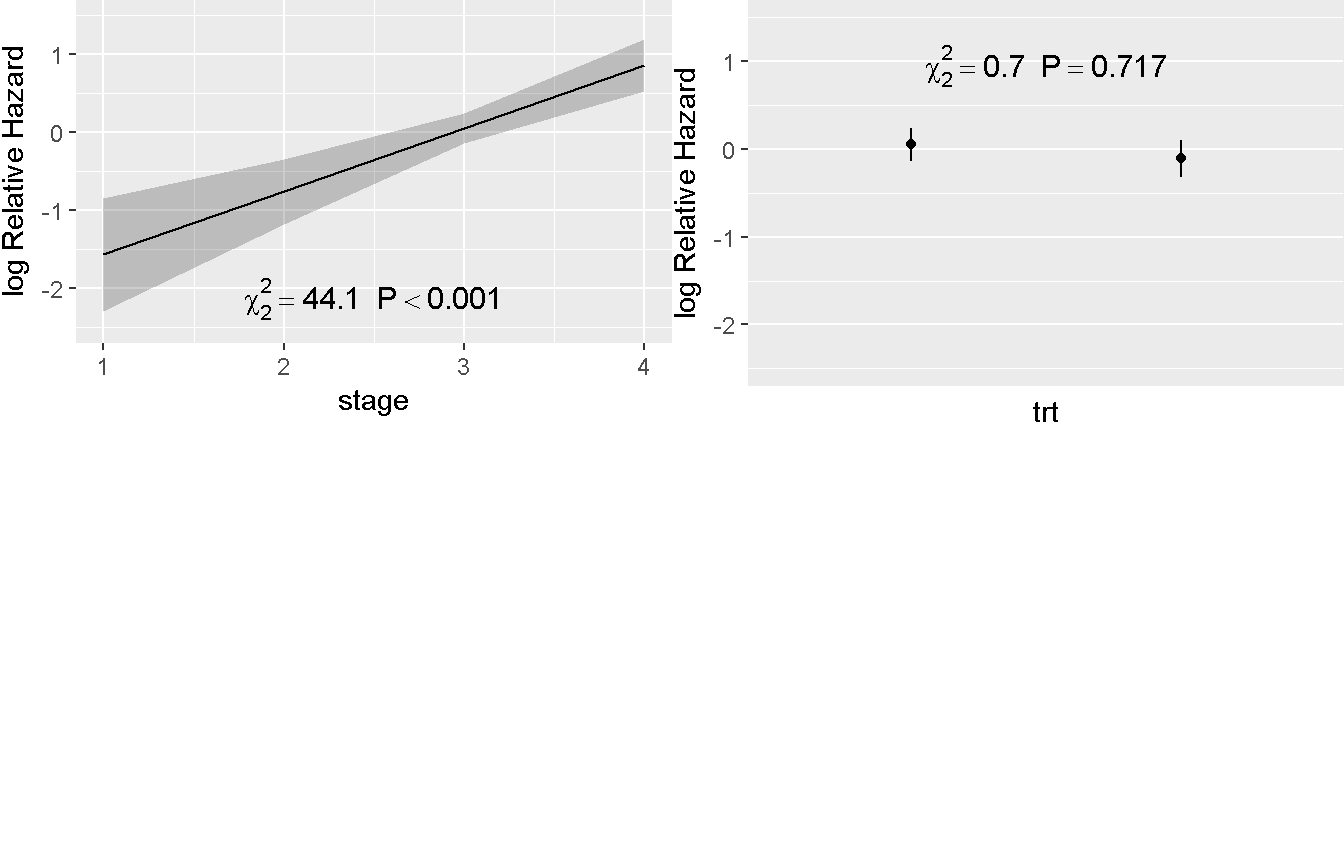
\includegraphics{SuDACDa-notes_files/figure-latex/unnamed-chunk-22-1.pdf}

\begin{Shaded}
\begin{Highlighting}[]
\KeywordTok{Predict}\NormalTok{(rms_trt_stage) %>%}
\StringTok{  }\KeywordTok{ggplot}\NormalTok{(}\DataTypeTok{anova =} \KeywordTok{anova}\NormalTok{(rms_trt_stage), }\DataTypeTok{pval =} \OtherTok{TRUE}\NormalTok{)}
\end{Highlighting}
\end{Shaded}

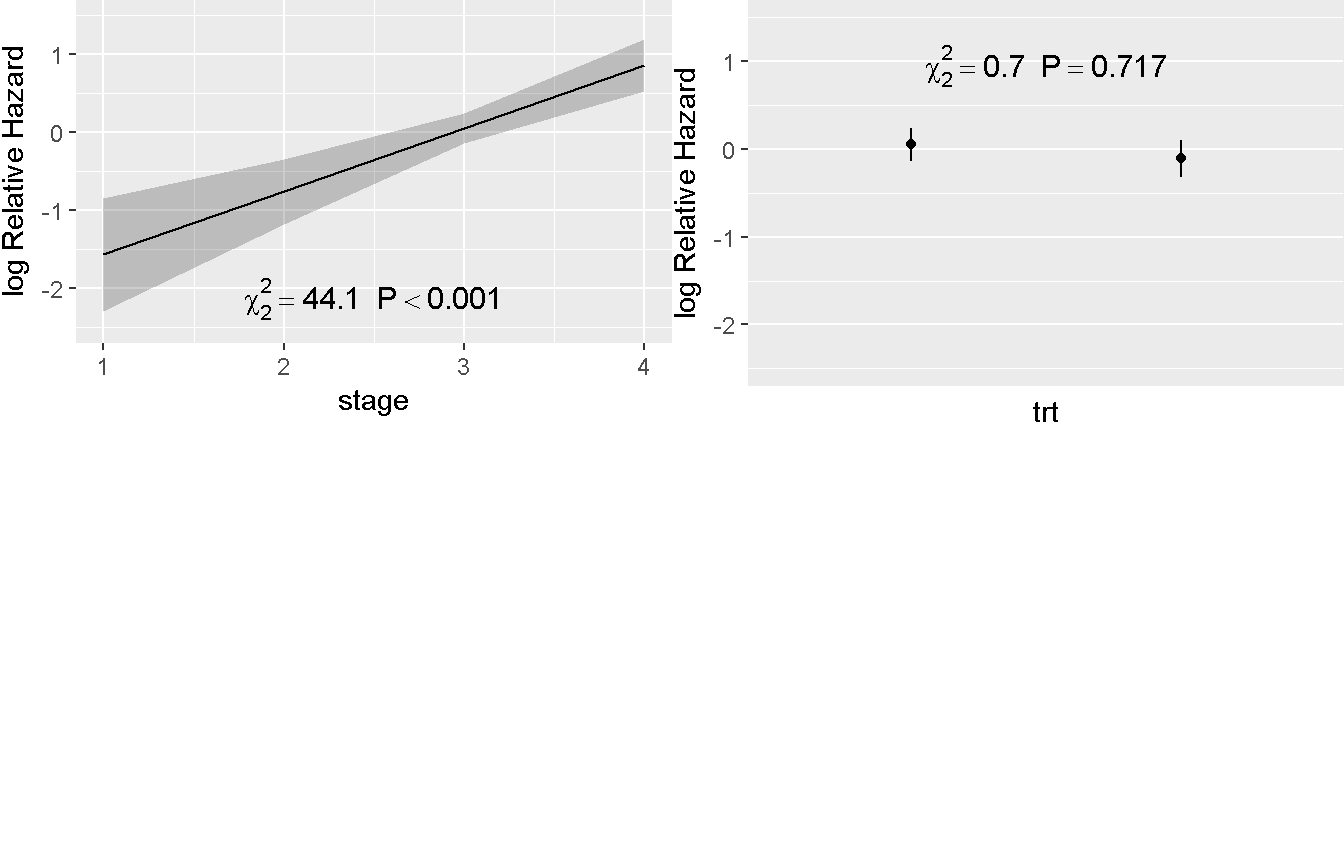
\includegraphics{SuDACDa-notes_files/figure-latex/unnamed-chunk-22-2.pdf}

Treatment continue to have no effect

\section{Longitudinal suvival data analayses}\label{longitudinal}

Load a data-set, update the \texttt{datadist()} for the \textbf{rms}
package, and take a look at the data

\begin{Shaded}
\begin{Highlighting}[]
\NormalTok{pbcseq_df <-}\StringTok{ }\KeywordTok{as_tibble}\NormalTok{(pbcseq)}
\NormalTok{dd <-}\StringTok{ }\KeywordTok{datadist}\NormalTok{(pbcseq_df)}

\NormalTok{pbcseq_df}
\end{Highlighting}
\end{Shaded}

\begin{verbatim}
## # A tibble: 1,945 x 19
##       id futime status   trt      age    sex   day ascites hepato spiders
##    <int>  <int>  <int> <int>    <dbl> <fctr> <int>   <int>  <int>   <int>
##  1     1    400      2     1 58.76523      f     0       1      1       1
##  2     1    400      2     1 58.76523      f   192       1      1       1
##  3     2   5169      0     1 56.44627      f     0       0      1       1
##  4     2   5169      0     1 56.44627      f   182       0      1       1
##  5     2   5169      0     1 56.44627      f   365       0      1       1
##  6     2   5169      0     1 56.44627      f   768       0      1       1
##  7     2   5169      0     1 56.44627      f  1790       1      1       1
##  8     2   5169      0     1 56.44627      f  2151       1      1       1
##  9     2   5169      0     1 56.44627      f  2515       1      1       1
## 10     2   5169      0     1 56.44627      f  2882       1      1       1
## # ... with 1,935 more rows, and 9 more variables: edema <dbl>, bili <dbl>,
## #   chol <int>, albumin <dbl>, alk.phos <int>, ast <dbl>, platelet <int>,
## #   protime <dbl>, stage <int>
\end{verbatim}

\begin{itemize}
\tightlist
\item
  The only tricky task is to correctly manage and prepare the data. Our
  proposal take advantage of the \texttt{dplyr} functionality
\end{itemize}

\begin{Shaded}
\begin{Highlighting}[]
\NormalTok{pbcseq_full <-}\StringTok{ }\NormalTok{pbcseq_df %>%}
\StringTok{  }\KeywordTok{group_by}\NormalTok{(id) %>%}\StringTok{                    }\CommentTok{# perform all the next according to the id}
\StringTok{  }\KeywordTok{mutate}\NormalTok{(}
    \DataTypeTok{start  =} \NormalTok{day,                                 }\CommentTok{# just to have consistent names}
    \DataTypeTok{end    =} \KeywordTok{lead}\NormalTok{(day),           }\CommentTok{# the end is "the next start" (last will be NA)}
    \DataTypeTok{status =} \KeywordTok{if_else}\NormalTok{(}\KeywordTok{is.na}\NormalTok{(end), status, 0L), }
    \DataTypeTok{end    =} \KeywordTok{if_else}\NormalTok{(}\KeywordTok{is.na}\NormalTok{(end), futime, end) }\CommentTok{# fill the NA-ends (i.e. the lasts)}
                                              \CommentTok{# with the real end}
\NormalTok{)}
\end{Highlighting}
\end{Shaded}

\subsection{Impact of bilurubine of death}\label{bilurubine2}

\begin{Shaded}
\begin{Highlighting}[]
\NormalTok{bil_mod <-}\StringTok{ }\KeywordTok{cph}\NormalTok{(}
  \KeywordTok{Surv}\NormalTok{(}\DataTypeTok{time =} \NormalTok{start, }\DataTypeTok{time2 =} \NormalTok{end, }\DataTypeTok{event =} \NormalTok{status ==}\StringTok{ }\NormalTok{2L) ~}\StringTok{ }\KeywordTok{log}\NormalTok{(bili),}
  \DataTypeTok{data =} \NormalTok{pbcseq_full,}
  \DataTypeTok{x    =} \OtherTok{TRUE}\NormalTok{,}
  \DataTypeTok{y    =} \OtherTok{TRUE}
\NormalTok{)}

\KeywordTok{summary}\NormalTok{(bil_mod)}
\end{Highlighting}
\end{Shaded}

\begin{verbatim}
##              Effects              Response : Surv(time = start, time2 = end, event = status == 2) 
## 
##  Factor        Low High Diff. Effect S.E.    Lower 0.95 Upper 0.95
##  bili          0.8 3.9  3.1   2.0410 0.13391 1.7786      2.3035   
##   Hazard Ratio 0.8 3.9  3.1   7.6984      NA 5.9213     10.0090
\end{verbatim}

\begin{Shaded}
\begin{Highlighting}[]
\KeywordTok{plot}\NormalTok{(}
  \DataTypeTok{x   =} \NormalTok{pbcseq_full$end,}
  \DataTypeTok{y   =} \KeywordTok{residuals}\NormalTok{(bil_mod, }\DataTypeTok{type =} \StringTok{'dfbeta'}\NormalTok{),}
  \DataTypeTok{col =} \StringTok{'red'}
\NormalTok{)}
\end{Highlighting}
\end{Shaded}

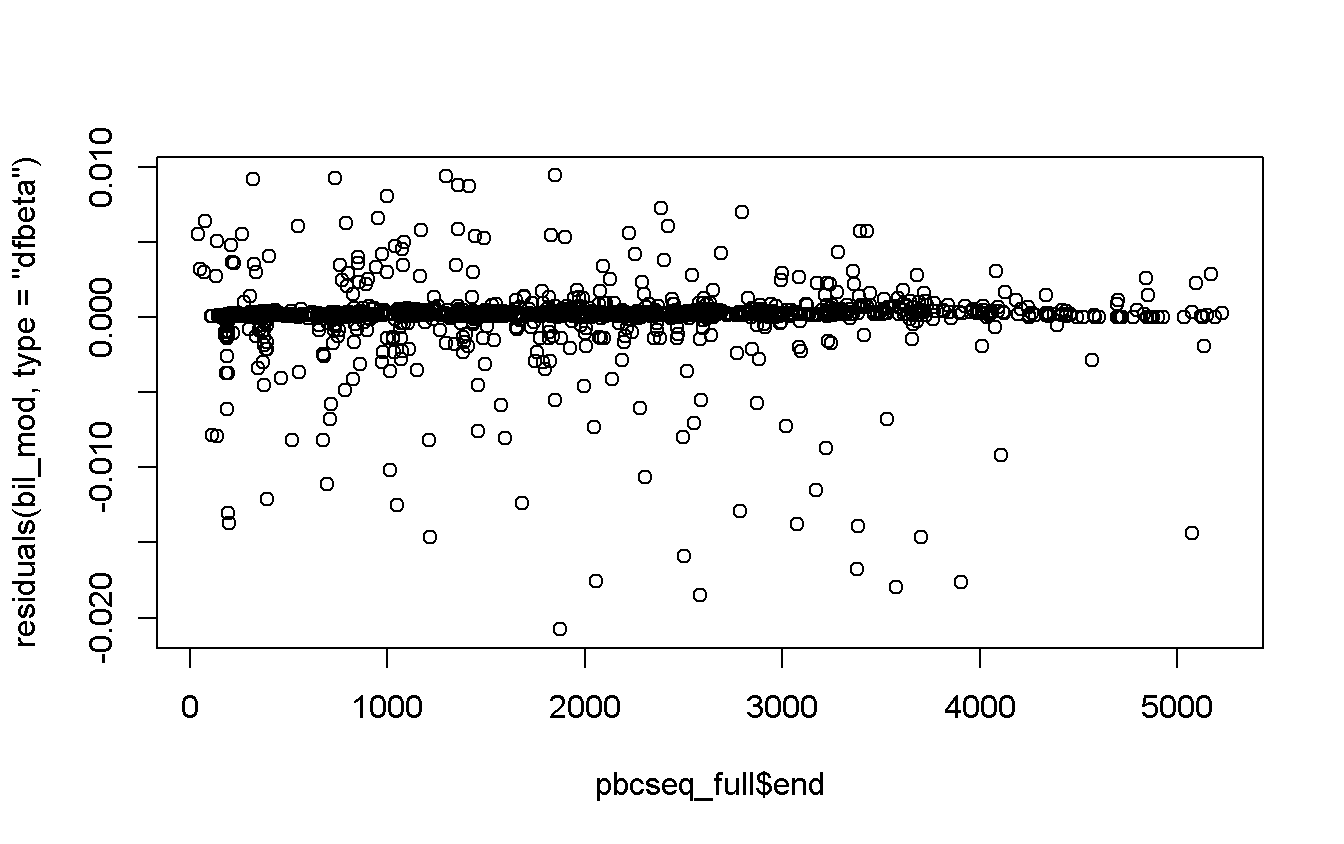
\includegraphics{SuDACDa-notes_files/figure-latex/unnamed-chunk-25-1.pdf}

\subsection{Impact of ast}\label{ast_full2}

\begin{Shaded}
\begin{Highlighting}[]
\NormalTok{ast_mod <-}\StringTok{ }\KeywordTok{cph}\NormalTok{(}
  \KeywordTok{Surv}\NormalTok{(}\DataTypeTok{time =} \NormalTok{start, }\DataTypeTok{time2 =} \NormalTok{end, }\DataTypeTok{event =} \NormalTok{status ==}\StringTok{ }\NormalTok{2L) ~}\StringTok{ }\NormalTok{ast,}
  \DataTypeTok{data =} \NormalTok{pbcseq_full,}
  \DataTypeTok{x    =} \OtherTok{TRUE}\NormalTok{,}
  \DataTypeTok{y    =} \OtherTok{TRUE}
\NormalTok{)}

\KeywordTok{summary}\NormalTok{(ast_mod)}
\end{Highlighting}
\end{Shaded}

\begin{verbatim}
##              Effects              Response : Surv(time = start, time2 = end, event = status == 2) 
## 
##  Factor        Low High Diff. Effect S.E.     Lower 0.95 Upper 0.95
##  ast           72  155  83    0.2875 0.044222 0.20083    0.37417   
##   Hazard Ratio 72  155  83    1.3331       NA 1.22240    1.45380
\end{verbatim}

\begin{Shaded}
\begin{Highlighting}[]
\KeywordTok{plot}\NormalTok{(}
  \DataTypeTok{x   =} \NormalTok{pbcseq_full$end,}
  \DataTypeTok{y   =} \KeywordTok{residuals}\NormalTok{(ast_mod, }\DataTypeTok{type =} \StringTok{'dfbeta'}\NormalTok{),}
  \DataTypeTok{col =} \StringTok{'red'}
\NormalTok{)}
\end{Highlighting}
\end{Shaded}

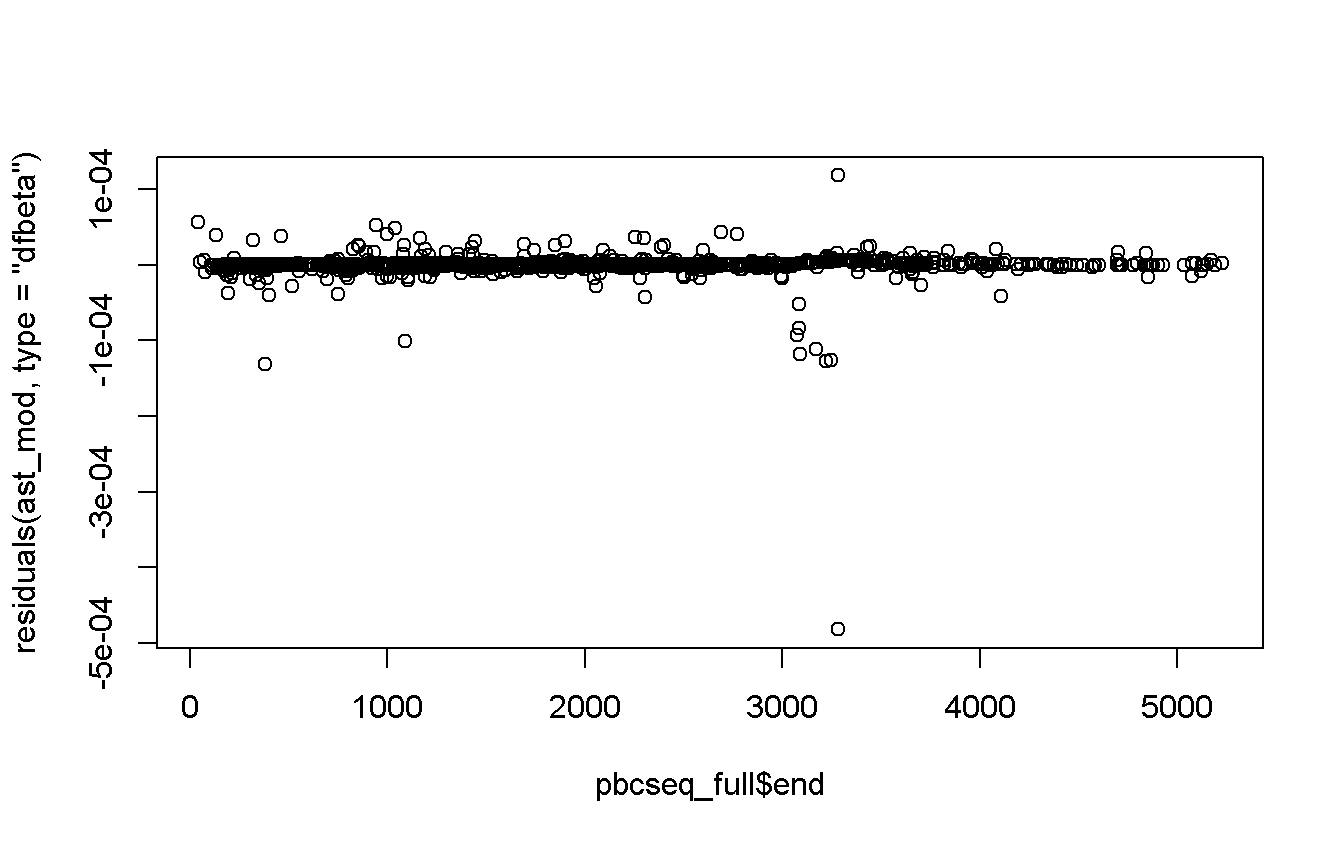
\includegraphics{SuDACDa-notes_files/figure-latex/unnamed-chunk-26-1.pdf}

\begin{Shaded}
\begin{Highlighting}[]
\KeywordTok{plot}\NormalTok{(}
  \DataTypeTok{x   =} \NormalTok{pbcseq_full$end,}
  \DataTypeTok{y   =} \KeywordTok{residuals}\NormalTok{(ast_mod, }\DataTypeTok{type =} \StringTok{'martingale'}\NormalTok{),}
  \DataTypeTok{col =} \StringTok{'brown'}
\NormalTok{)}
\end{Highlighting}
\end{Shaded}

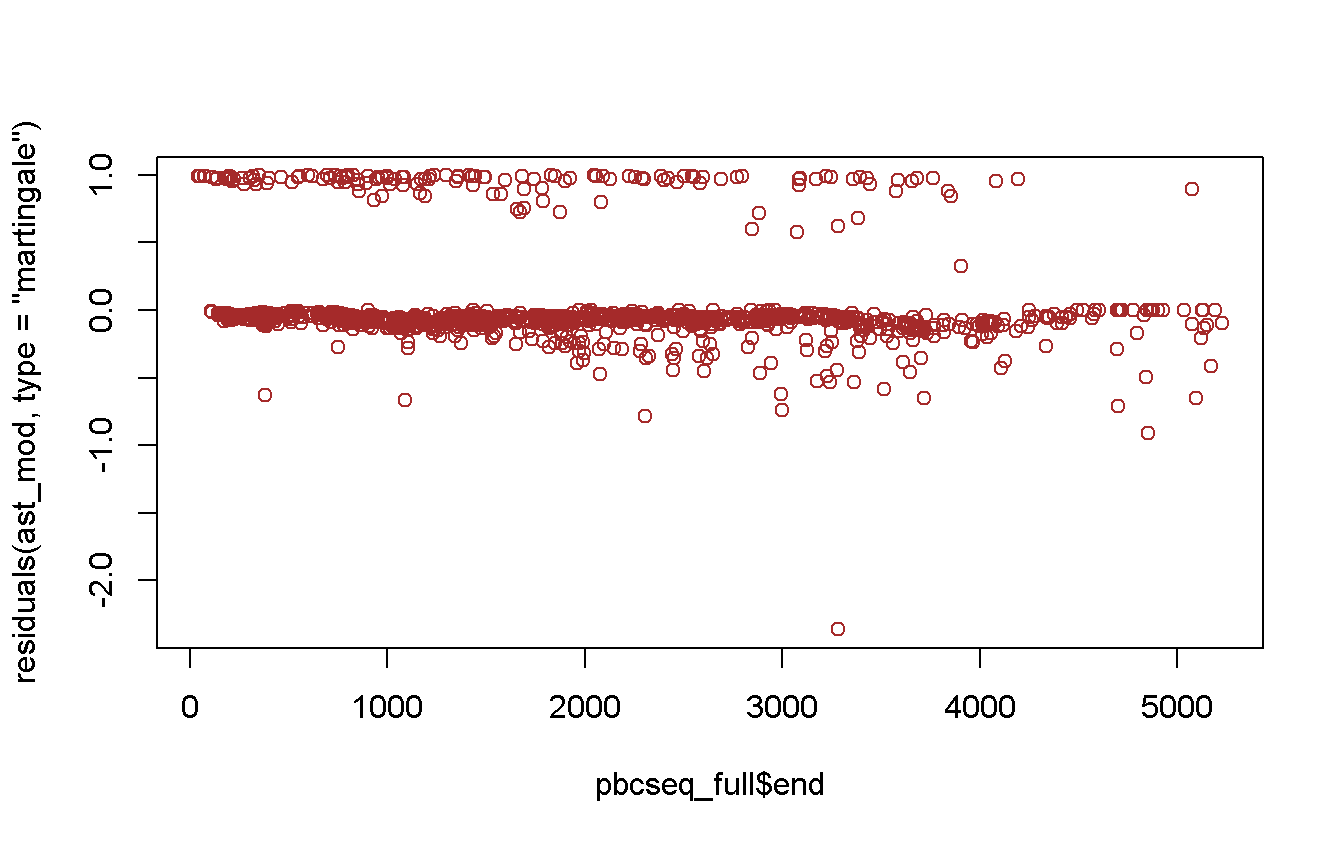
\includegraphics{SuDACDa-notes_files/figure-latex/unnamed-chunk-26-2.pdf}

What happen with the strange observations? We try to find which is that
outlier.

\begin{Shaded}
\begin{Highlighting}[]
\CommentTok{# look at the residual caracteristics}
\KeywordTok{residuals}\NormalTok{(ast_mod, }\DataTypeTok{type =} \StringTok{'martingale'}\NormalTok{) %>%}
\StringTok{  }\NormalTok{describe}
\end{Highlighting}
\end{Shaded}

\begin{verbatim}
## . 
##          n    missing   distinct       Info       Mean        Gmd 
##       1945          0       1855          1 -2.395e-17     0.1868 
##        .05        .10        .25        .50        .75        .90 
##   -0.16941   -0.11177   -0.07449   -0.05021   -0.03303   -0.01672 
##        .95 
##    0.95170 
## 
## lowest : -2.3632251 -0.9104219 -0.7874086 -0.7390614 -0.7120605
## highest:  0.9960346  0.9963091  0.9968442  0.9970148  0.9970895
\end{verbatim}

\begin{Shaded}
\begin{Highlighting}[]
\CommentTok{# take the id of the lowest}
\NormalTok{strange_id <-}\StringTok{ }\KeywordTok{residuals}\NormalTok{(ast_mod, }\DataTypeTok{type =} \StringTok{'martingale'}\NormalTok{) %>%}
\StringTok{  }\NormalTok{which.min}

\CommentTok{# take a look to the ast}
\NormalTok{pbcseq_full$ast %>%}\StringTok{ }\NormalTok{describe}
\end{Highlighting}
\end{Shaded}

\begin{verbatim}
## . 
##        n  missing distinct     Info     Mean      Gmd      .05      .10 
##     1945        0      418        1    122.7    74.42     41.9     51.2 
##      .25      .50      .75      .90      .95 
##     72.0    107.0    155.0    209.3    250.7 
## 
## lowest :    6.2   21.0   21.7   22.0   23.3, highest:  473.0  655.7  685.1  918.0 1205.0
\end{verbatim}

\begin{Shaded}
\begin{Highlighting}[]
\CommentTok{# check the id}
\NormalTok{pbcseq_full$ast[[strange_id]]}
\end{Highlighting}
\end{Shaded}

\begin{verbatim}
## [1] 1205
\end{verbatim}

Here is another example in which the opinion of a clinician is
mandatory, i.e.~we cannot decide if ignore outliers, which ones, etc

\section{Prognostic model}\label{prognostic2}

\subsection{\texorpdfstring{prognostic model with \texttt{àscites},
\texttt{edema}, \texttt{sex}, \texttt{bili}, \texttt{ast},
\texttt{platelet},
\texttt{stage}}{prognostic model with àscites, edema, sex, bili, ast, platelet, stage}}\label{prognostic-model-with-ascites-edema-sex-bili-ast-platelet-stage}

\begin{Shaded}
\begin{Highlighting}[]
\CommentTok{# prepare an ad hoc data frame}
\NormalTok{pbc_updated <-}\StringTok{ }\NormalTok{pbc_df %>%}\StringTok{ }
\StringTok{  }\KeywordTok{mutate}\NormalTok{(}
    \DataTypeTok{bili_log     =} \KeywordTok{log}\NormalTok{(bili),}
    \DataTypeTok{ast_log      =} \KeywordTok{log}\NormalTok{(ast),}
    \DataTypeTok{platelet_ref =} \NormalTok{platelet_ref, }\CommentTok{# we have already defined it}
    \DataTypeTok{stage_fct    =} \KeywordTok{as.factor}\NormalTok{(stage)}
  \NormalTok{)}

\NormalTok{dd <-}\StringTok{ }\KeywordTok{datadist}\NormalTok{(pbc_updated)}

\CommentTok{# take a look at them }
\NormalTok{pbc_updated %>%}\StringTok{ }
\StringTok{  }\NormalTok{dplyr::}\KeywordTok{select}\NormalTok{(}
    \NormalTok{ascites, edema, sex, bili_log, ast_log, platelet_ref, stage_fct}
  \NormalTok{) %>%}\StringTok{ }
\StringTok{  }\NormalTok{describe}
\end{Highlighting}
\end{Shaded}

\begin{verbatim}
## . 
## 
##  7  Variables      418  Observations
## ---------------------------------------------------------------------------
## ascites 
##        n  missing distinct     Info      Sum     Mean      Gmd 
##      312      106        2    0.213       24  0.07692   0.1425 
## 
## ---------------------------------------------------------------------------
## edema 
##        n  missing distinct     Info     Mean      Gmd 
##      418        0        3    0.391   0.1005   0.1756 
##                             
## Value        0.0   0.5   1.0
## Frequency    354    44    20
## Proportion 0.847 0.105 0.048
## ---------------------------------------------------------------------------
## sex 
##        n  missing distinct 
##      418        0        2 
##                       
## Value          m     f
## Frequency     44   374
## Proportion 0.105 0.895
## ---------------------------------------------------------------------------
## bili_log 
##        n  missing distinct     Info     Mean      Gmd      .05      .10 
##      418        0       98    0.998   0.5715    1.149  -0.6931  -0.5108 
##      .25      .50      .75      .90      .95 
##  -0.2231   0.3365   1.2238   2.0832   2.6391 
## 
## lowest : -1.2039728 -0.9162907 -0.6931472 -0.5108256 -0.3566749
## highest:  3.0726933  3.1135153  3.1986731  3.2386785  3.3322045
## ---------------------------------------------------------------------------
## ast_log 
##        n  missing distinct     Info     Mean      Gmd      .05      .10 
##      312      106      179        1     4.71   0.5075    3.994    4.102 
##      .25      .50      .75      .90      .95 
##    4.389    4.742    5.023    5.280    5.390 
## 
## lowest : 3.271468 3.345685 3.734092 3.770459 3.806662
## highest: 5.662960 5.700945 5.794841 5.823046 6.125230
## ---------------------------------------------------------------------------
## platelet_ref 
##        n  missing distinct 
##      407       11        3 
##                                               
## Value        (150,400]     (0,150] (400,1e+03]
## Frequency          311          61          35
## Proportion       0.764       0.150       0.086
## ---------------------------------------------------------------------------
## stage_fct 
##        n  missing distinct 
##      412        6        4 
##                                   
## Value          1     2     3     4
## Frequency     21    92   155   144
## Proportion 0.051 0.223 0.376 0.350
## ---------------------------------------------------------------------------
\end{verbatim}

There are 11 basic df (one each continuous variable and
one-minus-n-level for the categorical one), so to use all of them we
need at least \(110\) obs. Data has \(418\), this allow us to use a more
complex model, with some interaction, splines, etc (more or less other
\(15 -- 30\) df).

We decide (following suggestions from \citet{harrell2015regression}) to
consider splines for any continuous variable (with 3 knots) and consider
sex interaction with them and the other numerical variables, leading to
near \(20\) df.

\begin{Shaded}
\begin{Highlighting}[]
\NormalTok{data_used <-}\StringTok{ }\NormalTok{pbc_updated %>%}\StringTok{ }
\StringTok{  }\NormalTok{dplyr::}\KeywordTok{select}\NormalTok{(status, time,}
    \NormalTok{sex, ascites, edema, bili_log, ast_log, platelet_ref, stage_fct}
\NormalTok{)}

\NormalTok{dd <-}\StringTok{ }\KeywordTok{datadist}\NormalTok{(data_used)}


\CommentTok{# all the data-set}
\KeywordTok{cph}\NormalTok{(}
  \KeywordTok{Surv}\NormalTok{(time, status ==}\StringTok{ }\DecValTok{2}\NormalTok{) ~}
\StringTok{    }\NormalTok{sex *}\StringTok{ }\NormalTok{(ascites +}\StringTok{ }\NormalTok{edema +}\StringTok{ }\KeywordTok{rcs}\NormalTok{(bili_log, }\DecValTok{3}\NormalTok{) +}\StringTok{ }\KeywordTok{rcs}\NormalTok{(ast_log, }\DecValTok{3}\NormalTok{)) +}
\StringTok{    }\NormalTok{platelet_ref +}\StringTok{ }\NormalTok{stage_fct,}
  \DataTypeTok{data =} \NormalTok{data_used}
\NormalTok{) %>%}\StringTok{ }
\StringTok{  }\NormalTok{summary}
\end{Highlighting}
\end{Shaded}

\begin{verbatim}
##              Effects              Response : Surv(time, status == 2) 
## 
##  Factor                               Low      High   Diff.   Effect    
##  ascites                               0.00000 1.0000 1.00000  1.1613000
##   Hazard Ratio                         0.00000 1.0000 1.00000  3.1941000
##  edema                                 0.00000 1.0000 1.00000  0.6370800
##   Hazard Ratio                         0.00000 1.0000 1.00000  1.8910000
##  bili_log                             -0.22314 1.2238 1.44690  1.2273000
##   Hazard Ratio                        -0.22314 1.2238 1.44690  3.4120000
##  ast_log                               4.38950 5.0232 0.63372  0.3791100
##   Hazard Ratio                         4.38950 5.0232 0.63372  1.4610000
##  sex - m:f                             2.00000 1.0000      NA  2.0211000
##   Hazard Ratio                         2.00000 1.0000      NA  7.5463000
##  platelet_ref - (0,150]:(150,400]      1.00000 2.0000      NA  0.0907330
##   Hazard Ratio                         1.00000 2.0000      NA  1.0950000
##  platelet_ref - (400,1e+03]:(150,400]  1.00000 3.0000      NA  0.0059127
##   Hazard Ratio                         1.00000 3.0000      NA  1.0059000
##  stage_fct - 1:3                       3.00000 1.0000      NA -1.2551000
##   Hazard Ratio                         3.00000 1.0000      NA  0.2850400
##  stage_fct - 2:3                       3.00000 2.0000      NA -0.3858200
##   Hazard Ratio                         3.00000 2.0000      NA  0.6798900
##  stage_fct - 4:3                       3.00000 4.0000      NA  0.6523900
##   Hazard Ratio                         3.00000 4.0000      NA  1.9201000
##  S.E.    Lower 0.95 Upper 0.95
##  0.31762  0.538770   1.78380  
##       NA  1.713900   5.95260  
##  0.35904 -0.066626   1.34080  
##       NA  0.935550   3.82200  
##  0.28103  0.676490   1.77810  
##       NA  1.967000   5.91870  
##  0.18497  0.016587   0.74164  
##       NA  1.016700   2.09940  
##  0.54588  0.951150   3.09100  
##       NA  2.588700  21.99800  
##  0.25377 -0.406650   0.58812  
##       NA  0.665870   1.80060  
##  0.35526 -0.690380   0.70221  
##       NA  0.501380   2.01820  
##  1.03160 -3.277100   0.76682  
##       NA  0.037739   2.15290  
##  0.30581 -0.985210   0.21356  
##       NA  0.373360   1.23810  
##  0.23174  0.198190   1.10660  
##       NA  1.219200   3.02400  
## 
## Adjusted to: sex=f ascites=0 edema=0.5 bili_log=0.3364722 ast_log=4.74232
\end{verbatim}

\begin{Shaded}
\begin{Highlighting}[]
\CommentTok{# without missing data, and with beckward stepwise variable selection}
\KeywordTok{cph}\NormalTok{(}
  \KeywordTok{Surv}\NormalTok{(time, status ==}\StringTok{ }\DecValTok{2}\NormalTok{) ~}
\StringTok{    }\NormalTok{sex +}\StringTok{ }\NormalTok{ascites +}\StringTok{ }\NormalTok{edema +}\StringTok{ }\NormalTok{bili_log +}\StringTok{ }\NormalTok{ast_log +}\StringTok{ }\NormalTok{platelet_ref +}\StringTok{ }\NormalTok{stage_fct,}
  \DataTypeTok{data =} \NormalTok{pbc_updated %>%}\StringTok{ }
\StringTok{    }\KeywordTok{filter}\NormalTok{(}\KeywordTok{complete.cases}\NormalTok{(.))}
\NormalTok{) %>%}\StringTok{ }
\StringTok{  }\KeywordTok{step}\NormalTok{(}\DataTypeTok{trace =} \DecValTok{0}\NormalTok{) %>%}\StringTok{ }
\StringTok{  }\NormalTok{summary}
\end{Highlighting}
\end{Shaded}

\begin{verbatim}
##              Effects              Response : Surv(time, status == 2) 
## 
##  Factor          Low      High   Diff.  Effect   S.E.    Lower 0.95
##  ascites          0.00000 1.0000 1.0000  0.62140 0.33765 -0.040376 
##   Hazard Ratio    0.00000 1.0000 1.0000  1.86150      NA  0.960430 
##  edema            0.00000 1.0000 1.0000  1.18730 0.33082  0.538900 
##   Hazard Ratio    0.00000 1.0000 1.0000  3.27820      NA  1.714100 
##  bili_log        -0.22314 1.2238 1.4469  1.24480 0.15866  0.933880 
##   Hazard Ratio   -0.22314 1.2238 1.4469  3.47240      NA  2.544400 
##  sex - m:f        2.00000 1.0000     NA  0.52890 0.25407  0.030938 
##   Hazard Ratio    2.00000 1.0000     NA  1.69710      NA  1.031400 
##  stage_fct - 1:3  3.00000 1.0000     NA -1.48070 1.01500 -3.470100 
##   Hazard Ratio    3.00000 1.0000     NA  0.22748      NA  0.031115 
##  stage_fct - 2:3  3.00000 2.0000     NA -0.29414 0.31748 -0.916400 
##   Hazard Ratio    3.00000 2.0000     NA  0.74517      NA  0.399960 
##  stage_fct - 4:3  3.00000 4.0000     NA  0.53395 0.22987  0.083422 
##   Hazard Ratio    3.00000 4.0000     NA  1.70570      NA  1.087000 
##  Upper 0.95
##  1.28320   
##  3.60810   
##  1.83570   
##  6.26950   
##  1.55580   
##  4.73890   
##  1.02690   
##  2.79230   
##  0.50872   
##  1.66320   
##  0.32812   
##  1.38840   
##  0.98449   
##  2.67640
\end{verbatim}

\chapter{\texorpdfstring{\emph{Wednesday}: Competing
risk}{Wednesday: Competing risk}}\label{competing-risk}

\section{Key (operative) concepts}\label{key3}

\section{Data manipulation}\label{data-manipulation}

\begin{Shaded}
\begin{Highlighting}[]
\KeywordTok{set.seed}\NormalTok{(}\DecValTok{171004}\NormalTok{)}
\KeywordTok{data}\NormalTok{(mgus, }\DataTypeTok{package =} \StringTok{'survival'}\NormalTok{)}
\CommentTok{# ?mgus}

\NormalTok{mgus_df <-}\StringTok{ }\KeywordTok{as_tibble}\NormalTok{(mgus)}
\NormalTok{dd <-}\StringTok{ }\KeywordTok{datadist}\NormalTok{(mgus_df)}

\NormalTok{mgus_df}
\end{Highlighting}
\end{Shaded}

\begin{verbatim}
## # A tibble: 241 x 12
##       id   age    sex  dxyr   pcdx pctime futime death   alb creat   hgb
##  * <dbl> <dbl> <fctr> <dbl> <fctr>  <dbl>  <dbl> <dbl> <dbl> <dbl> <dbl>
##  1     1    78 female    68   <NA>     NA    748     1   2.8   1.2  11.5
##  2     2    73 female    66     LP   1310   6751     1    NA    NA    NA
##  3     3    87   male    68   <NA>     NA    277     1   2.2   1.1  11.2
##  4     4    86   male    69   <NA>     NA   1815     1   2.8   1.3  15.3
##  5     5    74 female    68   <NA>     NA   2587     1   3.0   0.8   9.8
##  6     6    81   male    68   <NA>     NA    563     1   2.9   0.9  11.5
##  7     7    72 female    68   <NA>     NA   1135     1   3.0   0.8  13.5
##  8     8    79 female    69   <NA>     NA   2016     1   3.1   0.8  15.5
##  9     9    85 female    70   <NA>     NA   2422     1   3.2   1.0  12.4
## 10    10    58   male    65   <NA>     NA   6155     1   3.5   1.0  14.8
## # ... with 231 more rows, and 1 more variables: mspike <dbl>
\end{verbatim}

\begin{enumerate}
\def\labelenumi{\arabic{enumi}.}
\tightlist
\item
  Find number of patient with malignancy (AKA transition), death (w/out
  malignancy) and Free of Events.
\end{enumerate}

\begin{Shaded}
\begin{Highlighting}[]
\NormalTok{mgus_df <-}\StringTok{ }\NormalTok{mgus_df %>%}\StringTok{ }
\StringTok{  }\KeywordTok{mutate}\NormalTok{(}
    \DataTypeTok{malignancy =} \NormalTok{!}\KeywordTok{is.na}\NormalTok{(pcdx)}
  \NormalTok{)}

\NormalTok{mgus_df %>%}\StringTok{ }
\StringTok{  }\KeywordTok{group_by}\NormalTok{(malignancy, death) %>%}\StringTok{ }
\StringTok{  }\KeywordTok{summarise}\NormalTok{(}\DataTypeTok{n =} \KeywordTok{n}\NormalTok{())}
\end{Highlighting}
\end{Shaded}

\begin{verbatim}
## # A tibble: 4 x 3
## # Groups:   malignancy [?]
##   malignancy death     n
##        <lgl> <dbl> <int>
## 1      FALSE     0    14
## 2      FALSE     1   163
## 3       TRUE     0     2
## 4       TRUE     1    62
\end{verbatim}

Patients with malignancy as a First Observed Event (FOE) are 64;
patients which experiment death as FOE are 163, while the ones FoE are
14. 163.

\begin{enumerate}
\def\labelenumi{\arabic{enumi}.}
\setcounter{enumi}{1}
\tightlist
\item
  Find the indicator for censored, malignancy and death
  (\texttt{indicator})
\item
  Find the time-to-event to use in the models (\texttt{time\_t})
\end{enumerate}

\begin{Shaded}
\begin{Highlighting}[]
\NormalTok{mgus_df <-}\StringTok{ }\NormalTok{mgus_df %>%}\StringTok{ }
\StringTok{  }\KeywordTok{mutate}\NormalTok{(}
    \DataTypeTok{indicator =} \KeywordTok{if_else}\NormalTok{(malignancy, }\DecValTok{1}\NormalTok{, }\DecValTok{2} \NormalTok{*}\StringTok{ }\NormalTok{death),}
    \DataTypeTok{time_t    =} \KeywordTok{pmin}\NormalTok{(futime, pctime, }\DataTypeTok{na.rm =} \OtherTok{TRUE}\NormalTok{)}
\NormalTok{)}

\NormalTok{mgus_df}
\end{Highlighting}
\end{Shaded}

\begin{verbatim}
## # A tibble: 241 x 15
##       id   age    sex  dxyr   pcdx pctime futime death   alb creat   hgb
##    <dbl> <dbl> <fctr> <dbl> <fctr>  <dbl>  <dbl> <dbl> <dbl> <dbl> <dbl>
##  1     1    78 female    68   <NA>     NA    748     1   2.8   1.2  11.5
##  2     2    73 female    66     LP   1310   6751     1    NA    NA    NA
##  3     3    87   male    68   <NA>     NA    277     1   2.2   1.1  11.2
##  4     4    86   male    69   <NA>     NA   1815     1   2.8   1.3  15.3
##  5     5    74 female    68   <NA>     NA   2587     1   3.0   0.8   9.8
##  6     6    81   male    68   <NA>     NA    563     1   2.9   0.9  11.5
##  7     7    72 female    68   <NA>     NA   1135     1   3.0   0.8  13.5
##  8     8    79 female    69   <NA>     NA   2016     1   3.1   0.8  15.5
##  9     9    85 female    70   <NA>     NA   2422     1   3.2   1.0  12.4
## 10    10    58   male    65   <NA>     NA   6155     1   3.5   1.0  14.8
## # ... with 231 more rows, and 4 more variables: mspike <dbl>,
## #   malignancy <lgl>, indicator <dbl>, time_t <dbl>
\end{verbatim}

\begin{enumerate}
\def\labelenumi{\arabic{enumi}.}
\setcounter{enumi}{3}
\tightlist
\item
  Estimate the naive K-M and the cumulative incidence functions
\end{enumerate}

\begin{Shaded}
\begin{Highlighting}[]
\CommentTok{# Using survival}
\KeywordTok{cuminc}\NormalTok{(mgus_df$time_t, mgus_df$indicator) %>%}\StringTok{                  }\CommentTok{# ?cmprsk::cuminc}
\StringTok{  }\KeywordTok{plot}\NormalTok{(                                                  }\CommentTok{# ?cmprsk:::plot.cuminc}
    \DataTypeTok{main    =} \StringTok{'Cumulative Incidence Estimates curves'}\NormalTok{,}
    \DataTypeTok{col     =} \KeywordTok{c}\NormalTok{(}\StringTok{'blue'}\NormalTok{, }\StringTok{'red'}\NormalTok{),}
    \DataTypeTok{xlab    =} \StringTok{'Days'}\NormalTok{,}
    \DataTypeTok{curvlab =} \KeywordTok{c}\NormalTok{(}\StringTok{'Transition'}\NormalTok{, }\StringTok{'Death'}\NormalTok{),}
    \DataTypeTok{wh      =} \KeywordTok{c}\NormalTok{(}\DecValTok{1}\NormalTok{, }\DecValTok{1}\NormalTok{)                                          }\CommentTok{# legend position}
\NormalTok{)}

\KeywordTok{survfit}\NormalTok{(}\KeywordTok{Surv}\NormalTok{(time_t, malignancy) ~}\StringTok{ }\DecValTok{1}\NormalTok{,        }\CommentTok{# using `rms::npsurv()` is the same}
  \DataTypeTok{data =} \NormalTok{mgus_df}
  \NormalTok{) %>%}\StringTok{ }
\StringTok{  }\KeywordTok{lines}\NormalTok{(                          }\CommentTok{# Use `lines()` to draw over the previous plot}
    \DataTypeTok{fun       =} \StringTok{'event'}\NormalTok{,                            }\CommentTok{# plot the cumulative events}
    \DataTypeTok{conf.int   =} \OtherTok{FALSE}\NormalTok{,}
    \DataTypeTok{col       =} \StringTok{'black'}\NormalTok{,}
    \DataTypeTok{lty       =} \DecValTok{3}
\NormalTok{)}
\KeywordTok{legend}\NormalTok{(}\DataTypeTok{x =} \DecValTok{1}\NormalTok{, }\DataTypeTok{y =} \FloatTok{0.86}\NormalTok{,}
  \DataTypeTok{legend =} \StringTok{'Naive K-M (Overestimation of Transitions)'}\NormalTok{,}
  \DataTypeTok{col    =} \StringTok{'black'}\NormalTok{,}
  \DataTypeTok{lty    =} \DecValTok{3}\NormalTok{,}
  \DataTypeTok{bty    =} \StringTok{'n'} \CommentTok{# remove box arround the legend (because we have to add an entry)}
\NormalTok{)}
\end{Highlighting}
\end{Shaded}

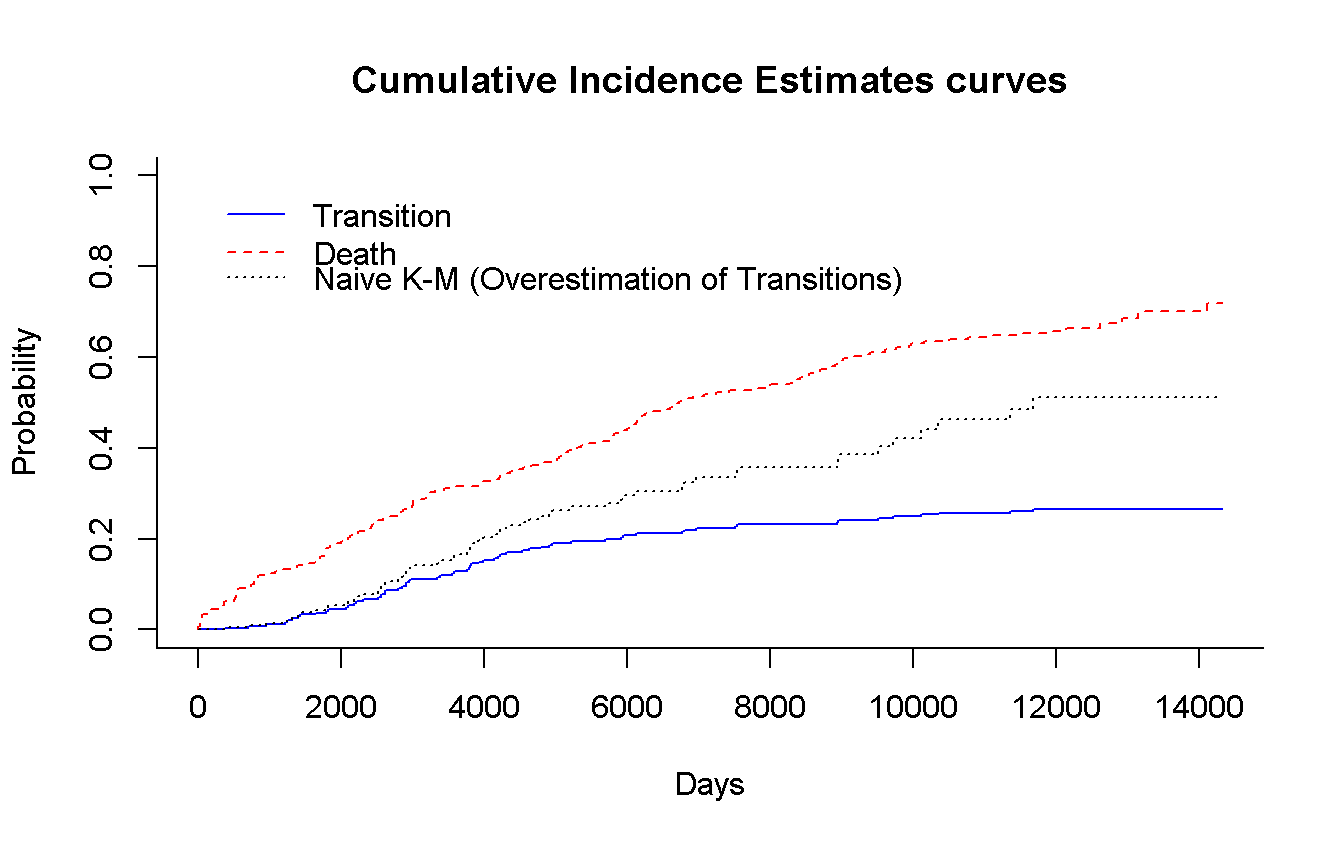
\includegraphics{SuDACDa-notes_files/figure-latex/unnamed-chunk-33-1.pdf}

\section{Simulation of Competing
risk}\label{simulation-of-competing-risk}

\begin{enumerate}
\def\labelenumi{\arabic{enumi}.}
\tightlist
\item
  Specify two cause-specific exponential hazard \(\lambda_1(t)\) and
  \(\lambda_2(t)\) of means \(0.8\) and \(1.2\). (Set sample size as you
  like.)
\end{enumerate}

\begin{Shaded}
\begin{Highlighting}[]
\NormalTok{n        <-}\StringTok{ }\FloatTok{1e4}
\NormalTok{lambda_1 <-}\StringTok{ }\FloatTok{0.8}
\NormalTok{lambda_2 <-}\StringTok{ }\FloatTok{1.2}
\end{Highlighting}
\end{Shaded}

\begin{enumerate}
\def\labelenumi{\arabic{enumi}.}
\setcounter{enumi}{1}
\tightlist
\item
  Simulate survival times \(T\) based on the all causes hazard
  \(\lambda_.(t) = \lambda_1(t) + \lambda_2(t)\).
\end{enumerate}

\begin{Shaded}
\begin{Highlighting}[]
\NormalTok{lambda    <-}\StringTok{ }\NormalTok{lambda_1 +}\StringTok{ }\NormalTok{lambda_2 }
\NormalTok{surv_time <-}\StringTok{ }\KeywordTok{rexp}\NormalTok{(n,}
  \DataTypeTok{rate =} \DecValTok{1} \NormalTok{/}\StringTok{ }\NormalTok{lambda}
\NormalTok{)}
\end{Highlighting}
\end{Shaded}

\begin{enumerate}
\def\labelenumi{\arabic{enumi}.}
\setcounter{enumi}{2}
\tightlist
\item
  Generate Bernoulli \(B(p)\) random variables, with
  \(p = \lambda_1(t) / \lambda_.(t)\), i.e.~is the probability of
  occurrence of the event of type 1.
\end{enumerate}

\begin{Shaded}
\begin{Highlighting}[]
\NormalTok{p_cens     <-}\StringTok{ }\NormalTok{lambda_1 /}\StringTok{ }\NormalTok{lambda}
\NormalTok{transition <-}\StringTok{ }\KeywordTok{rbinom}\NormalTok{(n,}
  \DataTypeTok{size =} \DecValTok{1}\NormalTok{,}
  \DataTypeTok{prob =} \NormalTok{p_cens}
\NormalTok{) %>%}
\StringTok{  }\NormalTok{as.logical     }\CommentTok{# Set as logical to use the variable for conditional statements}
\end{Highlighting}
\end{Shaded}

\begin{enumerate}
\def\labelenumi{\arabic{enumi}.}
\setcounter{enumi}{3}
\tightlist
\item
  Simulate uniform censoring times over \([0, 1]\).
\end{enumerate}

\begin{Shaded}
\begin{Highlighting}[]
\NormalTok{censor_time <-}\StringTok{ }\KeywordTok{runif}\NormalTok{(n,}
  \DataTypeTok{min =} \DecValTok{0}\NormalTok{,}
  \DataTypeTok{max =} \DecValTok{1}
\NormalTok{)}
\end{Highlighting}
\end{Shaded}

\begin{enumerate}
\def\labelenumi{\arabic{enumi}.}
\setcounter{enumi}{4}
\tightlist
\item
  Estimate the Cumulative Incidence of each competing event, with and
  without censoring; discuss the results.
\end{enumerate}

\begin{Shaded}
\begin{Highlighting}[]
\CommentTok{# create the dataset}
\NormalTok{sim_data <-}\StringTok{ }\KeywordTok{data_frame}\NormalTok{(}
  \DataTypeTok{id         =} \KeywordTok{seq_len}\NormalTok{(n),}
  \DataTypeTok{transition =} \NormalTok{transition,}
  \DataTypeTok{surv_t     =} \NormalTok{surv_time,}
  \DataTypeTok{cens_t     =} \NormalTok{censor_time,}
  \DataTypeTok{time_t     =} \KeywordTok{pmin}\NormalTok{(surv_t, cens_t),}
  \DataTypeTok{status     =} \KeywordTok{case_when}\NormalTok{(}
    \NormalTok{time_t ==}\StringTok{ }\NormalTok{cens_t ~}\StringTok{ }\NormalTok{0L,              }\CommentTok{# All the censored patients has status 0}
    \NormalTok{transition       ~}\StringTok{ }\NormalTok{1L,    }\CommentTok{# Among the other, the ones which has a transition}
                              \CommentTok{# have state 1}
    \OtherTok{TRUE}             \NormalTok{~}\StringTok{ }\NormalTok{2L     }\CommentTok{# All the other were dead (before the end of f-up)}
  \NormalTok{)}
\NormalTok{)}

\CommentTok{# Explore a (random) sample of three cases for each staus}
\NormalTok{sim_data %>%}\StringTok{ }
\StringTok{  }\KeywordTok{group_by}\NormalTok{(status) %>%}\StringTok{ }
\StringTok{  }\KeywordTok{sample_n}\NormalTok{(}\DecValTok{3}\NormalTok{)}
\end{Highlighting}
\end{Shaded}

\begin{verbatim}
## # A tibble: 9 x 6
## # Groups:   status [3]
##      id transition      surv_t    cens_t      time_t status
##   <int>      <lgl>       <dbl>     <dbl>       <dbl>  <int>
## 1  6759      FALSE 6.844765752 0.5175084 0.517508388      0
## 2   906       TRUE 1.378642827 0.5063402 0.506340163      0
## 3  3568       TRUE 0.623047318 0.5752797 0.575279657      0
## 4  2196       TRUE 0.506380841 0.9344626 0.506380841      1
## 5  8119       TRUE 0.157231928 0.9007847 0.157231928      1
## 6  5854       TRUE 0.742379822 0.8771130 0.742379822      1
## 7  1685      FALSE 0.539729742 0.9635529 0.539729742      2
## 8  4550      FALSE 0.001042022 0.3692372 0.001042022      2
## 9  6893      FALSE 0.410360153 0.9322769 0.410360153      2
\end{verbatim}

\begin{Shaded}
\begin{Highlighting}[]
\CommentTok{# Using survival}
\KeywordTok{cuminc}\NormalTok{(sim_data$time_t, sim_data$status) %>%}\StringTok{                  }\CommentTok{# ?cmprsk::cuminc}
\StringTok{  }\KeywordTok{plot}\NormalTok{(                                                  }\CommentTok{# ?cmprsk:::plot.cuminc}
    \DataTypeTok{main    =} \StringTok{'Cumulative Incidence Estimates curves'}\NormalTok{,}
    \DataTypeTok{col     =} \KeywordTok{c}\NormalTok{(}\StringTok{'blue'}\NormalTok{, }\StringTok{'red'}\NormalTok{),}
    \DataTypeTok{xlab    =} \StringTok{'Time (normalized [0, 1])'}\NormalTok{,}
    \DataTypeTok{curvlab =} \KeywordTok{c}\NormalTok{(}\StringTok{'Transition'}\NormalTok{, }\StringTok{'Event'}\NormalTok{),}
    \DataTypeTok{wh      =} \KeywordTok{c}\NormalTok{(}\FloatTok{0.01}\NormalTok{, }\DecValTok{1}\NormalTok{)                                          }\CommentTok{# legend position}
\NormalTok{)}

\KeywordTok{survfit}\NormalTok{(}\KeywordTok{Surv}\NormalTok{(time_t, transition) ~}\StringTok{ }\DecValTok{1}\NormalTok{,        }\CommentTok{# using `rms::npsurv()` is the same}
  \DataTypeTok{data =} \NormalTok{sim_data}
  \NormalTok{) %>%}\StringTok{ }
\StringTok{  }\KeywordTok{lines}\NormalTok{(                          }\CommentTok{# Use `lines()` to draw over the previous plot}
    \DataTypeTok{fun       =} \StringTok{'event'}\NormalTok{,                            }\CommentTok{# plot the cumulative events}
    \DataTypeTok{conf.int   =} \OtherTok{FALSE}\NormalTok{,}
    \DataTypeTok{col       =} \StringTok{'black'}\NormalTok{,}
    \DataTypeTok{lty       =} \DecValTok{3}
\NormalTok{)}
\KeywordTok{legend}\NormalTok{(}\DataTypeTok{x =} \FloatTok{0.01}\NormalTok{, }\DataTypeTok{y =} \FloatTok{0.86}\NormalTok{,}
  \DataTypeTok{legend =} \StringTok{'Naive K-M (overestimation of transitions)'}\NormalTok{,}
  \DataTypeTok{col    =} \StringTok{'black'}\NormalTok{,}
  \DataTypeTok{lty    =} \DecValTok{3}\NormalTok{,}
  \DataTypeTok{bty    =} \StringTok{'n'} \CommentTok{# remove box arround the legend (because we have to add an entry)}
\NormalTok{)}
\end{Highlighting}
\end{Shaded}

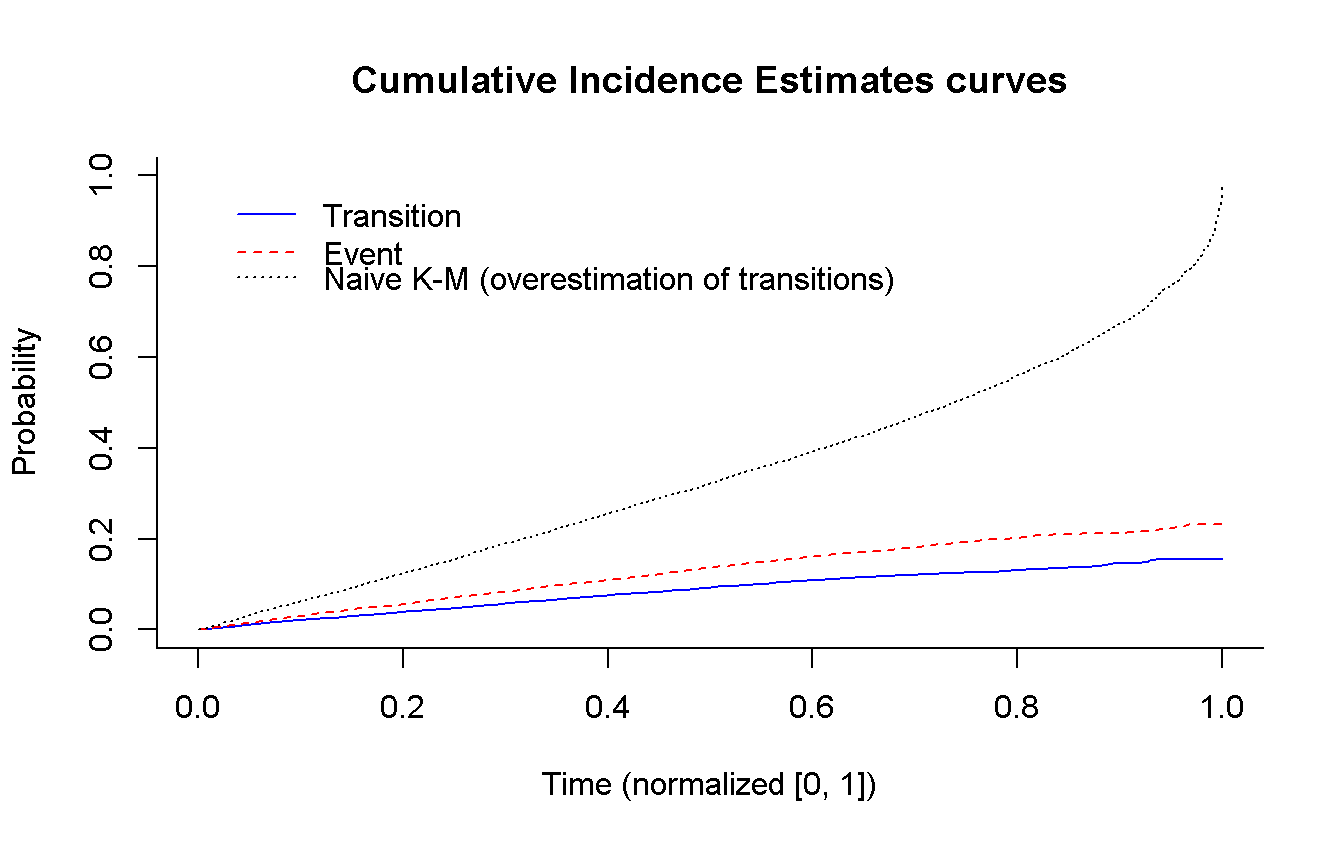
\includegraphics{SuDACDa-notes_files/figure-latex/unnamed-chunk-39-1.pdf}

\section{Estimation of the effect of sex on MGUS
incidence}\label{estimation-of-the-effect-of-sex-on-mgus-incidence}

\begin{enumerate}
\def\labelenumi{\arabic{enumi}.}
\tightlist
\item
  Compare the results of Cox cause specific hazard model\ldots{}
\end{enumerate}

\begin{quote}
For clinical questions, i.e.~cause specific risk to experiment the event
without taking into account the other couse(s)
\end{quote}

\begin{Shaded}
\begin{Highlighting}[]
\NormalTok{dd <-}\StringTok{ }\KeywordTok{datadist}\NormalTok{(mgus_df)}

\NormalTok{cox_sex <-}\StringTok{ }\KeywordTok{cph}\NormalTok{(}\KeywordTok{Surv}\NormalTok{(time_t, malignancy) ~}\StringTok{ }\NormalTok{sex,}
  \DataTypeTok{data =} \NormalTok{mgus_df,}
  \DataTypeTok{x    =} \OtherTok{TRUE}\NormalTok{,}
  \DataTypeTok{y    =} \OtherTok{TRUE}
\NormalTok{)}

\KeywordTok{summary}\NormalTok{(cox_sex)                  }\CommentTok{# this is good for a clean view of the effects}
\end{Highlighting}
\end{Shaded}

\begin{verbatim}
##              Effects              Response : Surv(time_t, malignancy) 
## 
##  Factor            Low High Diff. Effect   S.E.    Lower 0.95 Upper 0.95
##  sex - female:male 2   1    NA    0.049342 0.25103 -0.44268   0.54136   
##   Hazard Ratio     2   1    NA    1.050600      NA  0.64232   1.71830
\end{verbatim}

\begin{Shaded}
\begin{Highlighting}[]
\NormalTok{cox_sex                    }\CommentTok{# Here there are more informations (and the p-values)}
\end{Highlighting}
\end{Shaded}

\begin{verbatim}
## Cox Proportional Hazards Model
##  
##  cph(formula = Surv(time_t, malignancy) ~ sex, data = mgus_df, 
##      x = TRUE, y = TRUE)
##  
##                      Model Tests       Discrimination    
##                                           Indexes        
##  Obs       241    LR chi2      0.04    R2       0.000    
##  Events     64    d.f.            1    Dxy     -0.039    
##  Center -0.028    Pr(> chi2) 0.8441    g        0.024    
##                   Score chi2   0.04    gr       1.025    
##                   Pr(> chi2) 0.8441                      
##  
##           Coef    S.E.   Wald Z Pr(>|Z|)
##  sex=male -0.0493 0.2510 -0.20  0.8442  
## 
\end{verbatim}

\begin{Shaded}
\begin{Highlighting}[]
\KeywordTok{Predict}\NormalTok{(cox_sex) %>%}\StringTok{      }\CommentTok{# It is necessary to have the predictions for the plot}
\StringTok{  }\NormalTok{plot}
\end{Highlighting}
\end{Shaded}

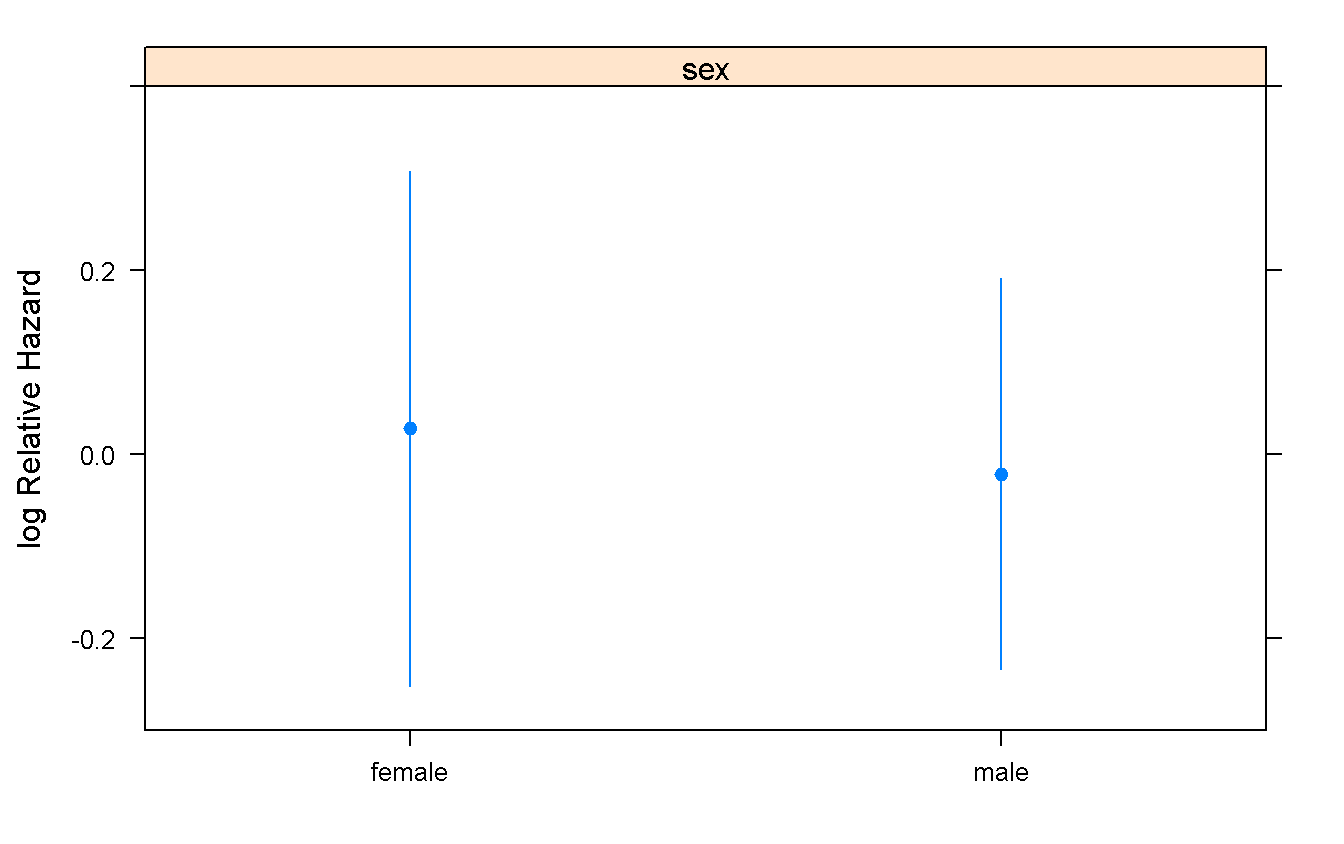
\includegraphics{SuDACDa-notes_files/figure-latex/unnamed-chunk-40-1.pdf}

\begin{Shaded}
\begin{Highlighting}[]
\NormalTok{cox_sex_death <-}\StringTok{ }\KeywordTok{cph}\NormalTok{(}\KeywordTok{Surv}\NormalTok{(time_t, indicator ==}\StringTok{ }\DecValTok{2}\NormalTok{) ~}\StringTok{ }\NormalTok{sex,}
  \DataTypeTok{data =} \NormalTok{mgus_df,}
  \DataTypeTok{x    =} \OtherTok{TRUE}\NormalTok{,}
  \DataTypeTok{y    =} \OtherTok{TRUE}
\NormalTok{)}

\KeywordTok{summary}\NormalTok{(cox_sex_death)}
\end{Highlighting}
\end{Shaded}

\begin{verbatim}
##              Effects              Response : Surv(time_t, indicator == 2) 
## 
##  Factor            Low High Diff. Effect   S.E.    Lower 0.95 Upper 0.95
##  sex - female:male 2   1    NA    -0.44221 0.16183 -0.75939   -0.12502  
##   Hazard Ratio     2   1    NA     0.64262      NA  0.46795    0.88248
\end{verbatim}

\begin{Shaded}
\begin{Highlighting}[]
\NormalTok{cox_sex_death}
\end{Highlighting}
\end{Shaded}

\begin{verbatim}
## Cox Proportional Hazards Model
##  
##  cph(formula = Surv(time_t, indicator == 2) ~ sex, data = mgus_df, 
##      x = TRUE, y = TRUE)
##  
##                      Model Tests       Discrimination    
##                                           Indexes        
##  Obs       241    LR chi2      7.65    R2       0.031    
##  Events    163    d.f.            1    Dxy      0.124    
##  Center 0.2514    Pr(> chi2) 0.0057    g        0.218    
##                   Score chi2   7.59    gr       1.243    
##                   Pr(> chi2) 0.0059                      
##  
##           Coef   S.E.   Wald Z Pr(>|Z|)
##  sex=male 0.4422 0.1618 2.73   0.0063  
## 
\end{verbatim}

\begin{Shaded}
\begin{Highlighting}[]
\KeywordTok{Predict}\NormalTok{(cox_sex_death) %>%}\StringTok{ }
\StringTok{  }\NormalTok{plot}
\end{Highlighting}
\end{Shaded}

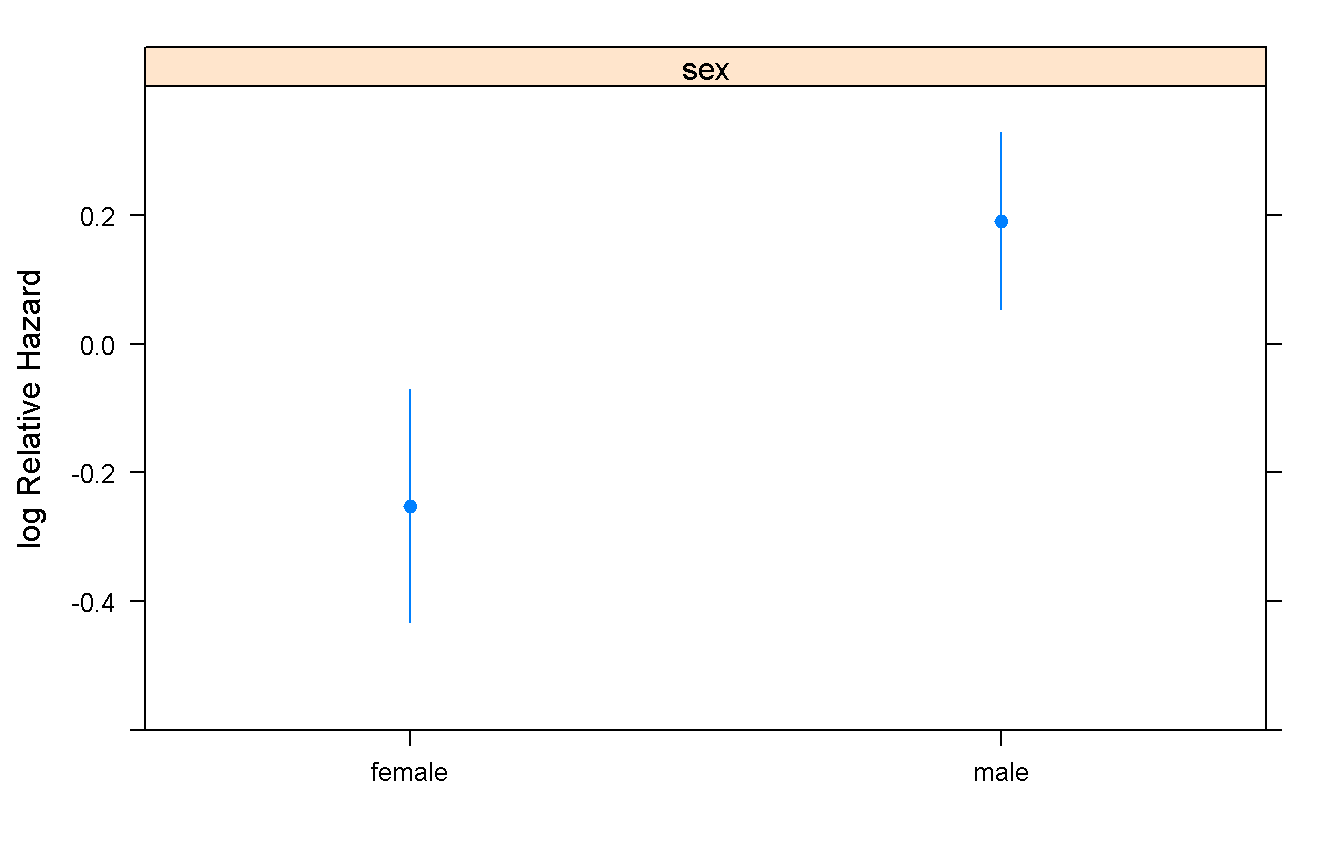
\includegraphics{SuDACDa-notes_files/figure-latex/unnamed-chunk-40-2.pdf}

\begin{enumerate}
\def\labelenumi{\arabic{enumi}.}
\setcounter{enumi}{1}
\tightlist
\item
  \ldots{}to those of the Fine and Gray model
\end{enumerate}

\begin{quote}
For administrative questions, i.e.~overall risk of experiment each event
taking into account the competing risk
\end{quote}

\begin{Shaded}
\begin{Highlighting}[]
\NormalTok{mgus_num <-}\StringTok{ }\NormalTok{mgus_df %>%}\StringTok{ }
\StringTok{  }\KeywordTok{mutate}\NormalTok{(}\DataTypeTok{sex =} \KeywordTok{as.numeric}\NormalTok{(sex))}

\KeywordTok{crr}\NormalTok{(}
  \DataTypeTok{ftime   =} \NormalTok{mgus_num$time_t,}
  \DataTypeTok{fstatus =} \NormalTok{mgus_num$indicator,}
  \DataTypeTok{cov1    =} \NormalTok{mgus_num$sex}
\NormalTok{) %>%}
\StringTok{  }\NormalTok{summary}
\end{Highlighting}
\end{Shaded}

\begin{verbatim}
## Competing Risks Regression
## 
## Call:
## crr(ftime = mgus_num$time_t, fstatus = mgus_num$indicator, cov1 = mgus_num$sex)
## 
##                 coef exp(coef) se(coef)     z p-value
## mgus_num$sex1 -0.339     0.713    0.249 -1.36    0.17
## 
##               exp(coef) exp(-coef)  2.5% 97.5%
## mgus_num$sex1     0.713        1.4 0.437  1.16
## 
## Num. cases = 241
## Pseudo Log-likelihood = -341 
## Pseudo likelihood ratio test = 1.83  on 1 df,
\end{verbatim}

\begin{Shaded}
\begin{Highlighting}[]
                                             \CommentTok{# here we do not have a way to plot }
\end{Highlighting}
\end{Shaded}

\chapter*{Software}\label{software}
\addcontentsline{toc}{chapter}{Software}

\section*{Packages}\label{packages}
\addcontentsline{toc}{section}{Packages}

All the exercise are solved using R (ver. 3.4.2) has been used provided
with packages: \texttt{survival} (\citet{R-survival}) for the survival
data analyses (reference package), \texttt{survminer}
(\citet{R-survminer}) for advance survival plot using \texttt{ggplot2}
(\citet{R-ggplot2}) package, \texttt{cmprsk} (\citet{R-cmprsk}) for
competing risk, \texttt{rms} (\citet{R-rms}) for additional features on
regression modeling strategies (survival ones included).

With regards to the data management, the collection of package
\texttt{tidyverse} (\citet{R-tidyverse}) is loaded, which includes:
\texttt{dplyr} (\citet{R-dplyr}) for data manipulation, \texttt{purrr}
(\citet{R-purrr}) for functional programming, \texttt{readr} (R-readr)
for data import, \texttt{tidyr} (R-tidyr) for funtions to tidy the data,
\texttt{tibble} (R-tibble) to take advantage of the \emph{tible} data
frame class and \texttt{ggplot2} as a interface for the Gramar of
Grahics.

The present book was written in RMarkdown (R-rmarkdown), compiled using
\texttt{knitr} (\citet{R-knitr}) and rendered as an HTML book by
\texttt{bookdown} (\citet{R-bookdown}).

\section*{System Information}\label{system-information}
\addcontentsline{toc}{section}{System Information}

All the code is compiled on a system with the following overall
characteristics and loaded packages.

\begin{Shaded}
\begin{Highlighting}[]
\NormalTok{devtools::}\KeywordTok{session_info}\NormalTok{()}
\end{Highlighting}
\end{Shaded}

\begin{verbatim}
##  setting  value                       
##  version  R version 3.4.2 (2017-09-28)
##  system   x86_64, mingw32             
##  ui       RTerm                       
##  language (EN)                        
##  collate  English_United States.1252  
##  tz       Europe/Berlin               
##  date     2017-10-04                  
## 
##  package      * version date       source        
##  acepack        1.4.1   2016-10-29 CRAN (R 3.4.1)
##  assertthat     0.2.0   2017-04-11 CRAN (R 3.4.1)
##  backports      1.1.0   2017-05-22 CRAN (R 3.4.0)
##  base         * 3.4.2   2017-09-28 local         
##  base64enc      0.1-3   2015-07-28 CRAN (R 3.4.0)
##  bindr          0.1     2016-11-13 CRAN (R 3.4.1)
##  bindrcpp     * 0.2     2017-06-17 CRAN (R 3.4.1)
##  bookdown       0.5     2017-08-20 CRAN (R 3.4.1)
##  broom          0.4.2   2017-02-13 CRAN (R 3.4.0)
##  cellranger     1.1.0   2016-07-27 CRAN (R 3.4.1)
##  checkmate      1.8.3   2017-07-03 CRAN (R 3.4.1)
##  cluster        2.0.6   2017-03-16 CRAN (R 3.4.1)
##  cmprsk       * 2.2-7   2014-06-17 CRAN (R 3.4.1)
##  codetools      0.2-15  2016-10-05 CRAN (R 3.4.0)
##  colorspace     1.3-2   2016-12-14 CRAN (R 3.4.1)
##  compiler       3.4.2   2017-09-28 local         
##  data.table     1.10.4  2017-02-01 CRAN (R 3.4.0)
##  datasets     * 3.4.2   2017-09-28 local         
##  devtools       1.13.3  2017-08-02 CRAN (R 3.4.1)
##  digest         0.6.12  2017-01-27 CRAN (R 3.4.1)
##  dplyr        * 0.7.3   2017-09-09 CRAN (R 3.4.1)
##  evaluate       0.10.1  2017-06-24 CRAN (R 3.4.1)
##  forcats        0.2.0   2017-01-23 CRAN (R 3.4.1)
##  foreign        0.8-69  2017-06-21 CRAN (R 3.4.0)
##  Formula      * 1.2-2   2017-07-10 CRAN (R 3.4.1)
##  ggplot2      * 2.2.1   2016-12-30 CRAN (R 3.4.1)
##  ggpubr       * 0.1.5   2017-08-22 CRAN (R 3.4.1)
##  glue           1.1.1   2017-06-21 CRAN (R 3.4.1)
##  graphics     * 3.4.2   2017-09-28 local         
##  grDevices    * 3.4.2   2017-09-28 local         
##  grid           3.4.2   2017-09-28 local         
##  gridExtra      2.3     2017-09-09 CRAN (R 3.4.1)
##  gtable         0.2.0   2016-02-26 CRAN (R 3.4.1)
##  haven          1.1.0   2017-07-09 CRAN (R 3.4.1)
##  Hmisc        * 4.0-3   2017-05-02 CRAN (R 3.4.1)
##  hms            0.3     2016-11-22 CRAN (R 3.4.1)
##  htmlTable      1.9     2017-01-26 CRAN (R 3.4.1)
##  htmltools      0.3.6   2017-04-28 CRAN (R 3.4.1)
##  htmlwidgets    0.9     2017-07-10 CRAN (R 3.4.1)
##  httr           1.3.1   2017-08-20 CRAN (R 3.4.1)
##  jsonlite       1.5     2017-06-01 CRAN (R 3.4.1)
##  km.ci          0.5-2   2009-08-30 CRAN (R 3.4.1)
##  KMsurv         0.1-5   2012-12-03 CRAN (R 3.4.0)
##  knitr          1.17    2017-08-10 CRAN (R 3.4.1)
##  labeling       0.3     2014-08-23 CRAN (R 3.4.0)
##  lattice      * 0.20-35 2017-03-25 CRAN (R 3.4.1)
##  latticeExtra   0.6-28  2016-02-09 CRAN (R 3.4.1)
##  lazyeval       0.2.0   2016-06-12 CRAN (R 3.4.1)
##  lubridate      1.6.0   2016-09-13 CRAN (R 3.4.1)
##  magrittr     * 1.5     2014-11-22 CRAN (R 3.4.1)
##  MASS           7.3-47  2017-04-21 CRAN (R 3.4.1)
##  Matrix         1.2-11  2017-08-16 CRAN (R 3.4.1)
##  MatrixModels   0.4-1   2015-08-22 CRAN (R 3.4.1)
##  memoise        1.1.0   2017-04-21 CRAN (R 3.4.1)
##  methods      * 3.4.2   2017-09-28 local         
##  mnormt         1.5-5   2016-10-15 CRAN (R 3.4.0)
##  modelr         0.1.1   2017-07-24 CRAN (R 3.4.1)
##  multcomp       1.4-7   2017-09-07 CRAN (R 3.4.1)
##  munsell        0.4.3   2016-02-13 CRAN (R 3.4.1)
##  mvtnorm        1.0-6   2017-03-02 CRAN (R 3.4.0)
##  nlme           3.1-131 2017-02-06 CRAN (R 3.4.1)
##  nnet           7.3-12  2016-02-02 CRAN (R 3.4.1)
##  parallel       3.4.2   2017-09-28 local         
##  pkgconfig      2.0.1   2017-03-21 CRAN (R 3.4.1)
##  plyr           1.8.4   2016-06-08 CRAN (R 3.4.1)
##  polspline      1.1.12  2015-07-14 CRAN (R 3.4.0)
##  psych          1.7.8   2017-09-09 CRAN (R 3.4.1)
##  purrr        * 0.2.3   2017-08-02 CRAN (R 3.4.1)
##  quantreg       5.33    2017-04-18 CRAN (R 3.4.1)
##  R6             2.2.2   2017-06-17 CRAN (R 3.4.1)
##  RColorBrewer   1.1-2   2014-12-07 CRAN (R 3.4.0)
##  Rcpp           0.12.12 2017-07-15 CRAN (R 3.4.1)
##  readr        * 1.1.1   2017-05-16 CRAN (R 3.4.1)
##  readxl         1.0.0   2017-04-18 CRAN (R 3.4.1)
##  reshape2       1.4.2   2016-10-22 CRAN (R 3.4.1)
##  rlang          0.1.2   2017-08-09 CRAN (R 3.4.1)
##  rmarkdown      1.6     2017-06-15 CRAN (R 3.4.1)
##  rms          * 5.1-1   2017-05-03 CRAN (R 3.4.1)
##  rpart          4.1-11  2017-04-21 CRAN (R 3.4.1)
##  rprojroot      1.2     2017-01-16 CRAN (R 3.4.1)
##  rstudioapi     0.7     2017-09-07 CRAN (R 3.4.1)
##  rvest          0.3.2   2016-06-17 CRAN (R 3.4.1)
##  sandwich       2.4-0   2017-07-26 CRAN (R 3.4.1)
##  scales         0.5.0   2017-08-24 CRAN (R 3.4.1)
##  SparseM      * 1.77    2017-04-23 CRAN (R 3.4.0)
##  splines        3.4.2   2017-09-28 local         
##  stats        * 3.4.2   2017-09-28 local         
##  stringi        1.1.5   2017-04-07 CRAN (R 3.4.0)
##  stringr        1.2.0   2017-02-18 CRAN (R 3.4.1)
##  survival     * 2.41-3  2017-04-04 CRAN (R 3.4.1)
##  survminer    * 0.4.0   2017-06-07 CRAN (R 3.4.1)
##  survMisc       0.5.4   2016-11-23 CRAN (R 3.4.1)
##  TH.data        1.0-8   2017-01-23 CRAN (R 3.4.1)
##  tibble       * 1.3.4   2017-08-22 CRAN (R 3.4.1)
##  tidyr        * 0.7.1   2017-09-01 CRAN (R 3.4.1)
##  tidyverse    * 1.1.1   2017-01-27 CRAN (R 3.4.1)
##  tools          3.4.2   2017-09-28 local         
##  utils        * 3.4.2   2017-09-28 local         
##  withr          2.0.0   2017-07-28 CRAN (R 3.4.1)
##  xml2           1.1.1   2017-01-24 CRAN (R 3.4.1)
##  xtable         1.8-2   2016-02-05 CRAN (R 3.4.1)
##  yaml           2.1.14  2016-11-12 CRAN (R 3.4.1)
##  zoo            1.8-0   2017-04-12 CRAN (R 3.4.1)
\end{verbatim}

\bibliography{packages,book}


\end{document}
